% Author: Jaron Mohammed.
% Figure paths rewritten from Claude Science artifact markers to local figs_full/.
% Full 55-page technical manuscript; the 6-page judge cut is clocks_to_coordinates.tex.
\documentclass[11pt]{article}

% ==================================================================
% BodyVector flagship manuscript
% Written against MANUSCRIPT_SPEC.md (locked-number ledger + framing rulebook).
% CONFIRMATORY TEST EXECUTED 2026-07-12: the single pre-registered CODE-15
% final-split M2-vs-M1 Cox LRT for D returned a NULL (HR 1.01/SD, p=0.48,
% n=74715, 2583 deaths; success criterion not met). The manuscript reports the
% executed result; the \pendingbox macro is retired. Every quantitative value is
% drawn from a frozen, verified artifact (see MANUSCRIPT_SPEC.md for version_ids;
% reveal artifacts CODE_CONFIRMATORY_RESULT.md 1dc242a4, reveal_result.json 3fb0fb63).
% ==================================================================

\usepackage[utf8]{inputenc}
\usepackage[T1]{fontenc}
\usepackage[margin=1in]{geometry}
\usepackage{amsmath,amssymb}
\usepackage{graphicx}
\usepackage{booktabs}
\usepackage{array}
\usepackage{siunitx}
\usepackage{authblk}
\usepackage{xcolor}
\usepackage{tcolorbox}
\usepackage[hidelinks]{hyperref}
\hypersetup{
  pdftitle={From Clocks to Coordinates: Controlled Human Perturbations Reveal Hidden Directions in ECG Biological Age},
  pdfauthor={Jaron Mohammed},
  pdfsubject={Biological aging; multi-clock decomposition; electrocardiography},
  pdfkeywords={biological age, shared axis, disagreement radius, ECG age, NHANES, cross-scale}
}
\usepackage[numbers,sort&compress]{natbib}
\usepackage{caption}
\captionsetup{font=small,labelfont=bf}
\sisetup{detect-weight=true,detect-family=true}

\newcommand{\D}{\ensuremath{D}}
\newcommand{\A}{\ensuremath{A}}
\newcommand{\Sq}{\ensuremath{\Sigma_q}}
\definecolor{pendinggray}{gray}{0.35}

% Marked confirmatory placeholder (used in Abstract and Results). The single
% pre-registered CODE-15 confirmatory test is NOT executed; no final-test
% mortality value has been read. This box is replaced only after the authorized reveal.
\title{\textbf{From Clocks to Coordinates: Controlled Human Perturbations Reveal
Hidden Directions in ECG Biological Age}}

\author[1,*]{Jaron Mohammed}
\affil[1]{University of Miami, Miami, FL, USA}
\affil[*]{Correspondence: jim4226@miami.edu}
\date{July 13, 2026}

\begin{document}
\maketitle

\begin{abstract}
\noindent
Neural ``ECG age'' and organ-age models return a single scalar, collapsing biophysically
distinct processes into one number. This work shows that a phase-resolved ECG-age
representation contains mechanism-aligned physiological \emph{directions} hidden by its
scalar output. Four phase-of-heartbeat age clocks (P, AV, QRS, ST-T)
compress into a \emph{shared axis} \A\ and an orthogonal \emph{disagreement radius} \D, with the
geometry frozen on CODE-15 \emph{before any outcome was read}. The radius \D\ was null on its
single pre-registered confirmatory mortality test (hazard ratio \num{1.01} per SD, 95\% CI
\numrange{0.98}{1.04}, $p=\num{0.48}$; $n=\num{74715}$, \num{2583} deaths)---the honest negative
that motivates a signed analysis. A randomized $I_{\text{Kr}}$ blocker (dofetilide) displaced the
ST-T repolarization clock ($+\num{4.2}$~SD$\cdot$h, false-discovery-rate $p=\num{0.002}$),
defining a covariance-scaled signed \emph{direction} $\mathbf{w}_{I_{\text{Kr}}}$---the coordinate
the unsigned radius discards. A second $I_{\text{Kr}}$ blocker (quinidine, $+\num{0.83}$ on the frozen axis) gave
within-cohort held-mechanism support, while the active multichannel comparators
ranolazine and verapamil projected more weakly with confidence intervals spanning zero;
the direction-derivation is exploratory (Holm-adjusted permutation $p=\num{0.069}$ across
the two screened perturbations). Frozen and
carried into an independent external cohort (Chapman--Shaoxing/Ningbo, $n=\num{44550}$, \num{386}
QT-extension cases), the direction added \emph{conditional} information about physician-assigned
QT-interval extension beyond conventional intervals, \A\ and \D\ (fully adjusted odds ratio
\num{1.23} per SD, 95\% CI \numrange{1.10}{1.36}, $p=\num{1.9e-4}$; marginally null, odds ratio
\num{1.00}---a suppression effect). The shared axis \A\ was separately robust and
mortality-associated (development hazard ratio \num{1.22} per SD) and generalized to whole-body
organ-system aging (NHANES, $+\num{1.21}$ per SD); the underlying whole-ECG clock additionally
reconstructed on a geographically distinct cohort ($r=\num{0.646}$ with chronological age),
whereas \A\ itself, a residual over age-adapted gaps, correlates with age only weakly there
($r=\num{0.26}$). The same shared-axis-versus-disagreement \emph{question} was then posed, as a
supporting multiscale atlas, across whole-body CT, brain MRI and an \emph{in-silico} genomic
screen---each with its own scale-appropriate decomposition rather than the electrical
(\A/\D/\S) geometry itself. Biological age is not one clock but a direction in a state space.
\end{abstract}

\section{Introduction}

Biological age is usually reported as one number. The central result of this study is that it is
better read as a \emph{direction} in a state space: a controlled human perturbation of a single
ion channel displaces the heartbeat's electrical age along a specific, reproducible axis that a
scalar age---and even an unsigned measure of subsystem disagreement---discards. That perturbation
discovery, developed in full for the electrical heartbeat, is the paper's contribution; the
whole-body and deep-time analyses that follow are a supporting multiscale atlas, applying the same
decomposition at other scales to show it is not an idiosyncrasy of the electrocardiogram, not
independent confirmation of the electrical result. Within a single lifetime, physiological
subsystems age at different rates, and the \emph{pattern} of that disagreement---not only its
average---may carry information; the electrical analysis makes this concrete and testable, and the
structural (whole-body CT) and genomic (human-accelerated DNA) scales, with the skeleton as a
literal bridge organ between the within-lifetime and deep-time views, illustrate the same
shared-axis/disagreement decomposition under one methodological stance: rigorous, outcome-blind,
open-data analysis, with no causal chain forced between scales. The electrical analysis occupies
the remainder of this introduction; the atlas scales follow in Parts~II and~III.

Machine-learning models that predict chronological age from a physiological
measurement---the 12-lead electrocardiogram, the blood proteome, a brain MRI---have
become a standard instrument of aging research \citep{lima2021,attia2019,tian2023,oh2023}.
The gap between predicted and true age is treated as a biomarker: a positive gap
means the system ``looks older'' than it is, and larger gaps predict disease and
death. Almost universally, however, these models return a single scalar. A whole-ECG
age clock compresses atrial, conduction, depolarization and repolarization
physiology---processes with distinct cellular substrates and distinct disease
associations---into one number, and a multi-organ age panel is typically read one
organ at a time or averaged into a composite \citep{oh2023,tian2023}. That organ
systems and brain-imaging views age heterogeneously, and that such heterogeneity tracks
mortality and disease, is by now well established---across organ-specific plasma clocks
\citep{oh2023,tian2023}, Mahalanobis physiological dysregulation \citep{cohen2013},
multimodal brain-age gaps \citep{wen2024}, and composite multi-system phenotypes that
already span brain, body and ECG \citep{li2025}; ECG-waveform localization of aging
effects has likewise been reported \citep{hempel2025}. A
scalar cannot express a hypothesis that is natural once several clocks exist: that
the \emph{pattern of disagreement} among subsystems, not only their common drift,
might carry information.

That intuition is formalized geometrically. Given $k$ subsystem age gaps measured on
the same individual, standardized against a healthy reference, two
coordinates are defined. The \emph{shared axis} \A\ is the projection onto the direction common
to all subsystems---the coordinated ``how old does the whole system look'' signal.
The \emph{disagreement radius} \D\ is the covariance-normalized Mahalanobis length of
the residual after the shared axis is removed---an unsigned measure of \emph{how much
the subsystems disagree}, calibrated so that its scale reflects the natural
covariation among clocks in health. \D\ is a score, not a direction: it discards the
sign of the disagreement and reports only its magnitude relative to the healthy
covariance ellipsoid. The two coordinates are constructed to be orthogonal, and---this
is the empirical question of the paper---they may answer different questions.

The idea of separating a shared component from an orthogonal residual is not itself
new: singular-value decompositions of mortality surfaces, residual scores in
multi-biomarker aging panels, and orthogonalized brain-age models all exploit a
version of it \citep{disco2025,cohen2013}. Neither is ECG age, nor multi-organ age, nor
multimodal brain-age, new \citep{lima2021,attia2019,tian2023,oh2023,ladejobi2021,wen2024,li2025},
and the broad claim that organs and imaging views age heterogeneously is by now crowded. What
has not, to the author's knowledge, been reported is (i) to train \emph{independent} age clocks for the individual
electrical phases of a single heartbeat, (ii) to compress them into a shared axis and
an orthogonal disagreement radius under a geometry frozen \emph{before any outcome is
read}, (iii) to ask, across multiple cohorts and physiological perturbations,
whether the shared axis and the disagreement radius carry \emph{dissociable}
information, and (iv) to recover the \emph{signed} coordinate the unsigned radius discards
as a covariance-scaled direction learned outcome-blind from a controlled ion-channel
perturbation, gated for stability and frozen for a pre-registered external test. That
recovered perturbation \emph{direction}---the coordinate the unsigned radius discards, frozen
and shown to transport to an external clinical phenotype---not any single clock, atlas or score,
is the contribution.

The dissociation is reported here under a strict outcome-blind protocol. The four phase clocks, the
shared axis \A, the disagreement radius \D\ and its healthy-reference covariance were
all fixed on the CODE-15 cohort without reading any mortality outcome; a four-volume
physical firewall and a split-before-partition patient hash enforced the separation
\citep{code15}. The frozen coordinates were then evaluated on: a locked CODE-15
development partition (mortality); the EchoNext cohort (echocardiographically
confirmed structural disease) \citep{echonext,poterucha2025}; a QT-prolonging drug challenge
(ECGRDVQ) \citep{ecgrdvq,johannesen2014} and controlled coronary occlusion (STAFF~III)
\citep{staff,martinez2017} as within-person physiological perturbations; the Chapman--Ningbo
cohort (geographic transfer) \citep{chapman}; and, at a different biological scale
entirely, NHANES organ-system aging linked to mortality \citep{nhanes}. The single
pre-registered confirmatory mortality test for the disagreement radius was executed once
on the locked CODE-15 final-test partition. The shared axis proved robust across
all of these settings; that the electrical disagreement radius showed no detectable
association with structure or acute stress across three pre-registered tests \emph{and} was null on the confirmatory
mortality test; and that a mixed model on the locked split assigns larger coefficients to
specific phase gaps (AV conduction and ST-T repolarization) than to their disagreement---a
hypothesis an external identifiable test did not support. Biological age is not one clock but a
direction in a state space.

\section{Part~I --- The electrical witness: a shared axis and an orthogonal disagreement radius}
\label{sec:parti}

Part~I develops the study's methodological core in full: independent age clocks for the
four electrical phases of the heartbeat, compressed into two orthogonal coordinates under a frozen,
outcome-blind geometry, and then carried unchanged to whole-body and brain-imaging scales.

\subsection{Two coordinates from four phase clocks}
\label{sec:construct}

Each median heartbeat was partitioned into four temporally disjoint windows
corresponding to atrial depolarization (P), atrioventricular conduction (AV,
measured on the $\text{P}_{\text{off}}\!\to\!\text{R}_{\text{on}}$ window),
ventricular depolarization (QRS) and ventricular repolarization (ST-T), and one
convolutional age regressor was trained per window (Fig.~\ref{fig:concept}A,B; Methods). Each
clock produces a per-subsystem age gap; standardizing the four gaps against a healthy
reference yields a vector $\mathbf{z}=(z_P,z_{AV},z_{QRS},z_{ST\text{-}T})$. A
unit-norm shared-axis direction $u=\tfrac12(1,1,1,1)^{\top}$ was fixed, defining the shared
axis as its projection $\A=u^{\top}\mathbf{z}=2\bar{z}$ (twice the mean gap), and the
disagreement radius $\D=\sqrt{\mathbf{q}^{\top}\Sigma_q^{-1}\mathbf{q}}$ as the
covariance-normalized length of the contrast vector $\mathbf{q}=C\mathbf{z}$ that lives
in the subspace orthogonal to $u$, where $\Sigma_q$ is the contrast covariance estimated
on the healthy subset used to fit the covariance ($n=\num{9338}$; Ledoit--Wolf shrinkage;
distinct from the larger $n=\num{9887}$ healthy calibration cohort on which the standardized
scores are later centred and scaled; Methods). By
construction $C u = 0$ and $CC^{\top}=I_3$, so \D\ is a radius \emph{within the contrast
subspace orthogonal to the shared direction}---it carries no shared-aging component---and
$\D^2$ follows a $\chi^2_3$ ideal under a standard-normal reference. (As a non-negative
scalar length, \D\ is not itself ``orthogonal'' to the scalar \A; the orthogonality is
between the shared direction and the contrast subspace \D\ summarizes.) All of these quantities---the clocks, $u_0$, $C$,
$\Sigma_q$ and the standardization constants---were frozen before any outcome was
read (Fig.~\ref{fig:concept}C). A ``concordant'' heart whose four gaps agree sits near
the centre of the healthy ellipsoid ($\D$ small) regardless of how old it looks;
a ``discordant'' heart in which one phase contrast dominates has a large $\D$
(Fig.~\ref{fig:concept}C).

\subsection{The shared axis \texorpdfstring{\A}{A} is consistently associated with aging across cohorts and scales}
\label{sec:shared}

The shared axis was associated with aging and its outcomes in every setting
examined (Fig.~\ref{fig:Arobust}); these associations were consistent across development,
secondary and transfer analyses, but \A\ was not itself the single pre-registered
confirmatory endpoint (\D\ was), so its incremental contribution was not adjudicated on a
locked split and the models below do not isolate \A's independent effect. On the locked CODE-15 development partition
($n=\num{61905}$, \num{2292} deaths, median follow-up \num{3.6}~years), \A\ carried
mortality risk with a hazard ratio of \num{1.22} per SD (95\% CI
\numrange{1.17}{1.27}, $p=\num{1.4e-20}$) adjusting for age and sex. In the EchoNext
cohort \A\ was associated with echocardiographically confirmed structural heart
disease (odds ratio \num{1.38} per SD in the frozen development model). Under
controlled balloon coronary occlusion in STAFF~III, \A\ rose sharply during ischemia
($+\num{0.64}$~SD, 95\% CI \numrange{0.33}{0.96}, $p<\num{0.001}$; whole-ECG apparent
age $+\num{3.8}$~years, 95\% CI \numrange{1.67}{6.00}, $p=\num{0.0008}$). The frozen
geometry also reconstructed without any refitting on the geographically distinct
Chapman--Ningbo cohort: the whole-ECG age clock that anchors the construction transferred
at correlation $r=\num{0.646}$ with chronological age ($n=\num{44595}$ with usable age;
predictive $R^2=\num{0.377}$, computed as $1-\text{SSE}/\text{SST}$ on the transferred age
scale, lower than $r^2$ because the untrained transfer carries a calibration slope and
offset). The shared axis \A\ is by construction a residual over age-adapted phase gaps
rather than an age predictor, so its own correlation with chronological age in this cohort
is low ($r=\num{0.26}$); the transfer evidence here is therefore that the frozen clocks and
geometry reconstruct out of distribution, not that \A\ predicts age. Finally, at a
completely different biological
scale, an analogous shared axis built from six organ-system age gaps in NHANES
carried mortality risk (hazard ratio \num{1.21} per SD, 95\% CI \numrange{1.13}{1.29},
$p=\num{2.0e-8}$, survey-weighted; \S\ref{sec:crossscale}). Across mortality,
structure, acute stress and organ scale, the coordinate common to all
subsystems was consistently associated with aging and its outcomes, and the frozen
construction additionally reconstructed on a geographically distinct cohort.

\subsection{The disagreement radius \texorpdfstring{\D}{D} shows no detectable association with structure or response to acute stress}
\label{sec:dissociation}

The hypothesis had been pre-registered that the disagreement radius would respond to
physiological stress and to structural disease---that stress or remodeling would drive
the phase clocks apart. In three independent pre-registered tests the radius showed no
detectable association with either, and the nulls are reported in full (Fig.~\ref{fig:Ddissoc}).

First, in EchoNext, the frozen four-phase disagreement score \D\ carried no
association with structural heart disease: adjusted odds ratio \num{1.00} per SD (95\%
CI \numrange{0.97}{1.04}), likelihood-ratio $p=\num{0.89}$, change in area under the
ROC curve $-\num{0.0001}$ ($n=\num{9687}$ final split, \num{3794} structural-disease
events). Second, in the ECGRDVQ crossover study, a supratherapeutic dose of the
QT-prolonging drug dofetilide did not move the composite radius \D\ relative to placebo (area under the
effect curve $-\num{1.88}$, 95\% CI $[-\num{4.56},\num{0.75}]$, $p=\num{0.16}$).
The signed phase decomposition behind \D, however, responded exactly as the drug's
mechanism predicts: dofetilide is a selective blocker of the rapid delayed-rectifier
potassium current $I_{\text{Kr}}$, which prolongs repolarization, and it displaced the
ST-T repolarization clock specifically (standardized AUEC $+\num{4.16}$, 95\% CI
\numrange{2.43}{5.86}, false-discovery-rate $q=\num{0.002}$; $n=\num{22}$ paired
crossovers) while the prespecified ventricular-depolarization (QRS) negative control did
not move ($+\num{0.28}$, $q=\num{0.84}$). The disagreement radius is null because it is
the covariance-normalized \emph{magnitude} of the phase-gap contrast vector: the unsigned
radius discards the \emph{direction} of a coherent one-phase displacement and retains only
its magnitude, so a physiologically-directed shift of a single phase clock need not register
as increased disagreement.
Third, in STAFF~III, acute ischemia produced no detectable change in \D\ (inflation minus baseline
$+\num{0.14}$~SD, 95\% CI $[-\num{0.30},\num{0.57}]$, $p=\num{0.54}$; recovery within the
prespecified $\pm 1$~SD equivalence margin by a two one-sided test). The
disagreement radius was also reproducible under repeated measurement on placebo within the
short ECGRDVQ crossover window (intraclass correlation, absolute agreement, $\num{0.83}$;
95\% CI \numrange{0.78}{0.87}), so within that controlled design the nulls are not
attributable to short-term measurement noise. This short-window reliability should not be
read as general person-level stability: across CODE-15 patients imaged on separate clinical
visits, \D\ was in fact the least reproducible coordinate the geometry defines (test--retest
$\mathrm{ICC}=\num{0.18}$; \S\ref{sec:robust}), so \D\ is a stable readout within a session
but a noisy person-level phenotype across visits.

These three nulls are the credential for \D, not a defeat: a covariance-normalized
disagreement score with no detectable association with structural disease and no detectable
change under two distinct acute stressors is, in these prespecified tests, a coordinate that
showed no detectable association with those axes. These are null tests, not demonstrated equivalence: the
STAFF interval ($-\num{0.30}$ to $+\num{0.57}$~SD) still permits a moderate ischemia effect,
and the drug-challenge and imaging arms had no prespecified equivalence margin, so the claim
is the absence of a detectable effect, not proof of exact invariance. As
\S\ref{sec:staff} shows, acute ischemia is in fact a coherent shift \emph{along} the
shared axis---which is precisely why the orthogonal disagreement radius does not move.
The single pre-registered confirmatory mortality test, reported in
\S\ref{sec:mortality}, was null in the same way: on the locked CODE-15 final split the
electrical disagreement radius carried no mortality information beyond age, sex, \A\
and a whole-ECG age clock ($\text{HR}=\num{1.01}$ per SD, $p=\num{0.48}$). The
electrical disagreement composite thus shows no detectable association on every
confirmatory-grade endpoint the study defined---structure, acute stress and
mortality---and its interest is precisely that consistency: it isolates what \emph{is}
informative (the shared axis, and specific phase gaps) by cleanly marking what is not.
A pre-registered secondary sensitivity score that excluded the atrial (P) phase showed
a small association with structural disease (odds ratio \num{1.05} per SD, 95\% CI
\numrange{1.02}{1.09}, $p=\num{0.0021}$, Holm-adjusted $\approx\num{0.006}$) but no
improvement in discrimination (change in AUC $+\num{0.0004}$, confidence interval
including zero); per the frozen protocol it was not promoted to a confirmatory
score, and is reported as an exploratory, phase-selective hypothesis for external
testing.

\subsection{The confirmatory mortality test is null}
\label{sec:mortality}

On the locked CODE-15 development partition, the disagreement radius had added a
statistically significant but quantitatively modest amount of mortality information
beyond age, sex, the shared axis \A\ and a previously published whole-ECG age clock
\citep{lima2021}: adding \D\ improved fit by a likelihood-ratio
$\chi^2=\num{9.77}$ ($p=\num{0.0018}$), hazard ratio \num{1.049} per SD
(95\% CI \numrange{1.021}{1.079}). This development association---used only to freeze
the model, never confirmatory---already attenuated when the four phase gaps were
modeled individually ($p=\num{0.26}$), hinting that the signal was concentrated in
specific phases rather than in ``disagreement'' as such.

The single pre-registered confirmatory test resolved that question. Executed once, on
the untouched final-test partition, behind the outcome firewall (Methods), the primary
M2-vs-M1 Cox likelihood-ratio test for \D\ was \textbf{null}: hazard ratio \num{1.010}
per SD (95\% CI \numrange{0.983}{1.039}), likelihood-ratio $\chi^2=\num{0.50}$,
$p=\num{0.48}$ ($n=\num{74715}$ complete cases, \num{2583} deaths, median follow-up
\num{3.4}~years). The frozen success criterion ($p<\num{0.05}$ and $\text{HR}>1$) was
not met. This is an informative rather than an inconclusive null: the confirmatory 95\%
confidence interval (ceiling \num{1.039} per SD) lies \emph{below} the development point
estimate (\num{1.049}), so the final split excludes a disagreement--mortality effect as
large as the one development had suggested. The prespecified sensitivity scores were
null in the same way (P-wave-excluded three-phase score $p=\num{0.20}$; AV-excluded
$p=\num{0.97}$), the diagnosis-adjusted model was null ($p=\num{0.54}$), proportional
hazards held (Schoenfeld $p=\num{0.29}$), and adding \D\ did not improve discrimination
(development-frozen concordance $\num{0.8071}\!\to\!\num{0.8072}$, $\Delta C=+\num{0.0001}$).

A prespecified phase-resolved decomposition (part of the frozen reveal, reported as a
secondary rather than as the single confirmatory primary) generates a hypothesis about
which phase gaps carry the association. In a secondary joint phase-gap model adjusted for age, sex, \D\ and the four
individual phase age gaps---but \emph{not} the separately trained whole-ECG
clock---the atrioventricular-conduction and ST-T-repolarization coefficients were positive
and large (AV hazard ratio \num{1.24} per SD, 95\% CI \numrange{1.19}{1.29},
$p=\num{3.1e-26}$; ST-T hazard ratio \num{1.13} per SD, 95\% CI \numrange{1.08}{1.17},
$p=\num{1.8e-9}$), whereas the atrial (P) and QRS coefficients were null (both
$p>\num{0.5}$); both large coefficients recur on an internal robustness partition
($p=\num{3.7e-21}$ and $p=\num{2.2e-7}$). This parameterization must be read with care.
Because the four gaps span the shared axis $\A=\tfrac12(z_P+z_{AV}+z_{QRS}+z_{STT})$, the
model contains the shared direction, but an individual phase coefficient is not an effect
at fixed \A: raising one gap while holding the others constant also changes \A. The
positive AV and ST-T coefficients therefore \emph{suggest} that directional, phase-specific
information carries risk, but this mixed shared-plus-contrast parameterization does not
establish phase-specific effects at fixed \A\ or beyond a whole-ECG clock. The rigorous
identifiable test---$M_{\text{base}}=\text{age}+\text{sex}+\text{whole-ECG age}+\A$ versus
$M_{\text{direction}}=M_{\text{base}}+q_1+q_2+q_3$ with a three-degree-of-freedom joint
likelihood-ratio test---requires re-opening the CODE-15 mortality labels, which the
single-use outcome firewall has now spent (Methods); it is prespecified future work.
An external, explicitly post-reveal version of that test was run in the independent
SaMi-Trop cohort (next paragraph), and was null. The complementary geometric
reading is that \D, an unsigned Mahalanobis magnitude over the contrast subspace, collapses
the signed phase contrasts into a single non-negative distance and so discards exactly the
directional information the phase-gap model highlights; a radial disagreement summary can
compress away directional signal, which is consistent with the confirmatory \D\ null.

To probe the phase-direction hypothesis without re-opening the spent CODE-15 firewall, the
frozen geometry was carried unchanged to an independent external cohort and tested once as a
declared post-reveal, exploratory analysis (protocol hash-locked before outcomes were read;
Methods). In SaMi-Trop \citep{cardoso2016samitrop,samitrop2021data}---a Chagas-disease cohort from
Brazil ($n=\num{1439}$ after a prespecified plausibility filter, \num{85} deaths, median
follow-up \num{2.1}~years)---the
identifiable directional model was fit: $M_{\text{base}}=\text{age}+\text{sex}+\text{whole-ECG
gap}+\A$ versus $M_{\text{direction}}=M_{\text{base}}+q_1+q_2+q_3$. The three-degree-of-freedom
joint likelihood-ratio test was \textbf{null} ($\chi^2=\num{2.75}$, $p=\num{0.43}$); no signed
contrast reached significance, and data-motivated AV-versus-others and ST-T-versus-others
contrasts were null after Holm correction (both $p>\num{0.5}$). The unsigned radius \D\ was
likewise null in this cohort (hazard ratio \num{1.03} per SD, $p=\num{0.36}$). The
development-grade AV/ST-T signal therefore did not replicate in an external cohort under a
frozen, identifiable model. With only \num{85} deaths this test is underpowered---the
confidence intervals on the signed contrasts are wide and do not exclude a moderate
effect---so it provides no positive external support for a transportable phase-direction
effect rather than firm evidence against one; a better-powered external replication is
required.

\subsection{The signed coordinate the radius discards defines a transportable perturbation direction}
\label{sec:transport}

That the radius \D\ is null on every confirmatory-grade endpoint---structure, acute
stress and mortality (\S\ref{sec:dissociation},~\S\ref{sec:mortality})---while the signed
decomposition recovers the drug's mechanism motivates a sharper construction: if the sign
carries the information the magnitude throws away, that sign should define a fixed,
transportable axis rather than a per-analysis finding. In whitened coordinates
$\hat{\mathbf{u}}=\Sigma_q^{-1/2}\mathbf{q}$ the radius is the length
$\D_{\text{raw}}=\lVert\hat{\mathbf{u}}\rVert$; a signed perturbation score is the
projection of $\hat{\mathbf{u}}$ onto a fixed unit axis, so $|S_{\text{raw}}|\le\D_{\text{raw}}$
for every exam by construction (Fig.~\ref{fig:compass}c). This bound is a geometric fact about
the \emph{raw} whitened coordinates $S_{\text{raw}}$ and $\D_{\text{raw}}$; the reported
standardized scores $S_{I_{\text{Kr}}}$ and \D\ are each separately z-scored on the frozen
calibration cohort, so the inequality need not hold between the standardized values. The question is whether a perturbation with known biology
yields a \emph{stable enough} axis to freeze and carry into an untouched cohort.

A covariance-scaled signed direction was learned outcome-blind from the $I_{\text{Kr}}$
blockade contrast (dofetilide minus placebo, ECGRDVQ, $n=\num{22}$ participants):
$\mathbf{w}_{I_{\text{Kr}}}=\Sigma_q^{-1}\mathbf{m}/\sqrt{\mathbf{m}^{\top}\Sigma_q^{-1}\mathbf{m}}$,
scaled so that $\mathbf{w}^{\top}\Sigma_q\mathbf{w}=1$. Its mean displacement was
dominated by the ST-T-versus-QRS contrast coordinate, consistent with selective
repolarization prolongation. Two candidate perturbations were screened for a stable,
freezable direction---the $I_{\text{Kr}}$ blockade contrast and, below, acute ischemia---so
this direction-derivation step is treated as \textbf{exploratory} and its statistics are
multiplicity-corrected across the two candidates; the confirmatory weight rests on the
independent external phenotype test that follows, not on the derivation. Stability was read
out on four descriptive criteria: pipeline yield, the participant-bootstrap covariance-aware
cosine $\cos_\Sigma$ with the full-sample direction and its lower bound, sign stability, and
a treatment-label sign-flip permutation. The $I_{\text{Kr}}$ direction was highly stable in
direction: the bootstrap median $\cos_\Sigma$ with the full-sample axis was \num{0.94} (95\%
CI \numrange{0.63}{1.00}), and \num{9999} of \num{10000} participant bootstraps reproduced its
sign without any alignment (\SI{99.99}{\percent} sign-stable; bootstrap directions were aligned
only for the visualization in Fig.~\ref{fig:compass}a, never for this count). Its magnitude was
also non-random, though only nominally so once multiplicity is accounted for: the sign-flip
permutation gave $p=\num{0.034}$, which is $p=\num{0.069}$ after Holm correction for the two
screened directions---suggestive rather than confirmatory, and the reason the derivation is
labelled exploratory. It was confirmed within the same crossover
cohort by a second, held-mechanism $I_{\text{Kr}}$ blocker, quinidine: the mean quinidine
projection on the frozen direction was $+\num{0.84}$ (95\% CI \numrange{0.52}{1.20},
bootstrap $p<\num{e-4}$), the two blockers were aligned in the whitened metric
($\cos_\Sigma=\num{0.94}$), and a leave-one-participant-out reconstruction was highly
stable (median $\cos_\Sigma=\num{0.997}$, minimum \num{0.95}). Two non-$I_{\text{Kr}}$
active comparators projected weakly and with intervals including zero (ranolazine
$+\num{0.21}$; verapamil $+\num{0.12}$), consistent with an $I_{\text{Kr}}$-dominant
direction rather than a response to drug exposure in general (Fig.~\ref{fig:compass}b).

The same gate was applied to acute ischemia and it \emph{failed} (bootstrap median
$\cos_\Sigma=\num{0.63}$ with an interval spanning zero; sign stable in only
\SI{79}{\percent} of bootstraps; permutation $p=\num{0.84}$): ischemia displaces the
phase-age vector coherently along the shared axis \A\ (\S\ref{sec:staff}), leaving no
stable contrast-subspace direction to freeze. Per the frozen protocol no substitute
direction was constructed, so the transportable ``atlas'' contains a single
retrospectively derived, exploratory perturbation direction ($k=1$), frozen before
the external transport test but not itself a pre-registered hypothesis. The signed score was then standardized (mean $\mu$, SD $\sigma$) on the frozen healthy
calibration cohort---the larger $n=\num{9887}$ cohort on which \D\ is also standardized, not the
smaller $n=\num{9338}$ subset used to estimate $\Sigma_q$ ($\mu=\num{0.008}$,
$\sigma=\num{1.01}$, $n=\num{9887}$).

The frozen axis was then carried, unchanged, into an independent external cohort with a
clinical phenotype: the combined Chapman--Shaoxing and Ningbo 12-lead databases
($n=\num{44550}$ with usable records; \num{386} carrying the physician-assigned
QT-interval-extension label, SNOMED~111975006). The pre-registered test was a
one-degree-of-freedom likelihood-ratio comparison for the standardized $I_{\text{Kr}}$ score
in a logistic model of QT extension adjusting for age, sex, heart rate, QTc, QRS, whole-ECG
age, \A\ and \D. The result is a \emph{conditional} (suppression) effect, and the adjustment
ladder is the point: marginally the frozen score is null (odds ratio \num{1.00} per SD,
$p=\num{0.996}$), it strengthens monotonically as conventional context is added
(age/sex OR \num{1.09}, $p=\num{0.09}$; $+$intervals OR \num{1.15}, $p=\num{0.007}$), and in
the fully adjusted model it is clearly non-null (OR \num{1.23} per SD, 95\% CI
\numrange{1.10}{1.36}, likelihood-ratio $p=\num{1.9e-4}$; identical under a Firth
penalized fit; Fig.~\ref{fig:chapman}). In other words the frozen $I_{\text{Kr}}$ direction adds information about
physician-assigned QT extension \emph{beyond} conventional intervals, the shared displacement
\A\ and the radial disagreement \D---it is a shape coordinate unmasked by adjustment, not a
marginally separable one. The pooled association was driven primarily by the larger Ningbo site
(\num{329} cases, OR \num{1.20}, $p=\num{0.002}$), which is part of the combined primary cohort and
so is a site-stratified estimate, not an independent replication; Chapman--Shaoxing pointed the same way but
is underpowered (\num{57} cases, OR \num{1.44}, 95\% CI \numrange{1.06}{1.97}, reported without
a pass/fail verdict). It was not, however, independent of rhythm context: it held when atrial
flutter/fibrillation were excluded ($p=\num{0.014}$) but attenuated to null when both flutter
and sinus bradycardia were removed ($p=\num{0.48}$, \num{86} cases), a limitation reported in
full. A reliable-QT subgroup filter (QTc \SIrange{350}{600}{\milli\second}, heart rate
\SIrange{40}{120}{\text{bpm}}) is a post-hoc robustness check, labelled as such and not
pre-registered. The frozen score is not claimed to be \emph{stronger} than QTc, \A\ or \D:
its incremental information is real (bootstrap incremental likelihood-ratio CI excludes zero)
but is not statistically distinguishable from those scalars. The defensible claim is narrow
and external: a direction frozen from a randomized drug perturbation carries conditional
information about an independent clinical QT phenotype, beyond conventional measurements.

\subsection{Acute ischemia is a coherent shift of the shared axis, not a loss of coordination}
\label{sec:staff}

STAFF~III records the 12-lead ECG before, during and after elective balloon coronary
occlusion, providing a within-person model of acute, reversible ischemia (\num{91}
occlusions in \num{70} patients). This experiment resolves \emph{why} the disagreement
radius shows no detectable change under stress (Fig.~\ref{fig:staff}). During occlusion all four phase
clocks moved in the same direction by similar amounts: the AV, QRS and ST-T gaps rose
significantly (AV $+\num{0.52}$~SD, false-discovery-rate $q=\num{0.009}$; QRS
$+\num{0.49}$, $q=\num{0.004}$; ST-T $+\num{0.47}$, $q=\num{0.037}$) and the atrial
gap rose non-significantly ($+\num{0.40}$, $q=\num{0.20}$). A coordinated positive
displacement of all four clocks is, by construction, a shift \emph{along} the shared
axis \A\ (which duly rose $+\num{0.64}$~SD) and \emph{not} a change in their
disagreement, so the component orthogonal to \A---whose magnitude is \D---was
statistically unchanged. The apparent phase-clock
displacement persisted into the \numrange{30}{40}-second reperfusion window (\A\
recovery minus baseline $+\num{0.59}$~SD, $p<\num{0.001}$), while the recovery-versus-baseline
change in \D\ was statistically equivalent to zero (\num{0.00}~SD, two one-sided tests
against a $\pm\num{1.0}$~SD margin, \SI{90}{\percent}~CI \numrange{-0.32}{0.31}). This is, to be clear, an \emph{apparent}
displacement of an age-trained readout under acute ischemia, not literal biological
aging over minutes; its value here is mechanistic---it shows directly that a strong
physiological perturbation loads onto the shared axis and produces no detectable
change in the disagreement radius, exactly as the geometry predicts.

\subsection{The electrical construct is internally valid, externally transferable and differs in reproducibility}
\label{sec:robust}
The analyses in this subsection were computed \emph{after} the single pre-registered
confirmatory test and are reported as post-hoc; each is either a re-presentation of the
already-locked mortality numbers or a no-outcome computation on frozen scores, so none
re-opens the confirmatory endpoint. All ran through the frozen scoring pipeline with no
refitting (geometry hash \texttt{5a3d8800\dots ee8e3e0}; Methods).

First, the phase clocks encode more than the classical interval durations they might be
suspected of merely re-reading. After adjusting for age and sex, each predicted phase age
was only weakly correlated with its matched standard interval (partial Spearman $\rho$,
CODE-15 calibration set, $n=\num{74715}$): P-clock versus P-duration $\rho=-\num{0.11}$,
AV-clock versus PR-interval $\rho=-\num{0.13}$, ST-T-clock versus QTc $\rho=+\num{0.08}$,
and only the QRS-clock read its interval appreciably ($\rho=+\num{0.20}$). The AV clock---which
carried the largest development-split mortality coefficient---is if anything \emph{weakly negatively} related to the PR
interval, so what it contributes is not a re-badging of classical PR prolongation
(Supplementary~Fig.~\ref{fig:s9}b).

Second, the frozen geometry reconstructs on an untrained external cohort. Applying the
fixed standardization, contrast basis and disagreement metric to Chapman--Shaoxing/Ningbo
(a 12-lead cohort used to train no clock and fit no calibration constant), the whole-ECG
age clock transferred at $r=\num{0.64}$ and all four phase clocks transferred positively
($n=\num{44595}$ with usable age; QRS $r=\num{0.57}$, P $r=\num{0.52}$, ST-T $r=\num{0.46}$,
AV $r=\num{0.34}$). On the subset entering the disagreement-geometry analysis
($n=\num{44550}$ after \D-score quality control), the shared axis and disagreement radius
were nearly uncorrelated ($r=-\num{0.17}$), as expected from their construction on
orthogonal subspaces. External disagreement was lowest in atrial-fibrillation/flutter records,
consistent with delineation-driven behavior rather than a coordination signal. These
cohorts carry no mortality follow-up comparable to CODE-15, so this establishes generality
of the age-structure geometry only, not an external mortality replication
(Supplementary~Fig.~\ref{fig:s9}c).

Third, the equal-weight shared axis is close to the direction the data would have chosen.
The pre-registered axis uses fixed weights $u=\tfrac12(1,1,1,1)$; a data-driven first
principal component of the four calibration z-scores (development split, $n=\num{61905}$;
$\num{51.5}\%$ of variance) has weights $(\num{0.45},\num{0.51},\num{0.51},\num{0.53})$---cosine
similarity $\num{0.998}$ with the fixed axis, and per-exam scores correlating at
$r=\num{0.9995}$. The choice made before any outcome was read is essentially the empirical
principal direction, so the axis is both interpretable and data-consistent.

Finally, the coordinates differ sharply in within-patient reproducibility. Across
$\num{66474}$ CODE-15 patients with $\ge 2$ QC-passing ECGs ($\num{177336}$ exams), the
composite disagreement radius \D\ was the \emph{least} reproducible coordinate the geometry
defines (test--retest $\mathrm{ICC}(1,1)=\num{0.18}$), well below the shared axis \A\
($\num{0.41}$) and every single-phase gap (QRS $\num{0.47}$, ST-T $\num{0.38}$, P
$\num{0.32}$, AV $\num{0.31}$). A Mahalanobis radius over a mixture of signal and noise
channels compounds measurement error, so this is a mechanistic complement to the null: \D\
is not only uninformative for mortality, it is the noisiest coordinate defined. The AV
gap carried a large development-split coefficient despite only moderate reproducibility
($\mathrm{ICC}=\num{0.31}$), which is consistent with a reproducible within-patient measurement rather than a
reliability artifact, though the external identifiable test did not support it. CODE-15 lacks per-exam acquisition dates, so this quantifies
within-patient measurement stability, not calendar drift of the coordinate; longitudinal
trajectory modeling of \A\ requires dated repeat exams and is left to future work
(Supplementary~Fig.~\ref{fig:s9}d).

\subsection{The same multiscale question extends across the body}
\label{sec:crossscale}

If the shared-axis/disagreement-radius decomposition captures something general about
biological aging rather than an idiosyncrasy of the electrocardiogram, the same
construction should behave similarly at a completely different scale. An
analogous BodyVector was built from six organ-system age gaps in NHANES 2005--2010 linked to
2019 mortality (\num{14362} participants, \num{1739} deaths, \num{160493}
person-years, median follow-up \num{11.3}~years), using survey-weighted Cox regression
with cross-fitted clocks (Fig.~\ref{fig:atlas}; Methods). The pattern reproduced the
heartbeat-scale result. The shared body axis $\A_{\text{body}}$ carried mortality
(hazard ratio \num{1.21} per SD, 95\% CI \numrange{1.13}{1.29}, $p=\num{2.0e-8}$), and
the body disagreement radius $\D_{\text{body}}$ added mortality information beyond it
(hazard ratio \num{1.21} per SD, 95\% CI \numrange{1.108}{1.328}, $p=\num{3.1e-5}$;
cross-validated concordance improvement $+\num{0.0041}$, 95\% CI
\numrange{0.0029}{0.0054}).\footnote{The $\D_{\text{body}}$ interval
\numrange{1.108}{1.328} is the design-based survey Cox estimate (\texttt{svycoxph},
combined-cycle MEC weights, robust standard errors, design degrees of freedom~47),
which is the appropriate model for the NHANES Linked Mortality File and matches the
canonical released Cox table; a naïve non-survey Cox model yields a narrower nominal
interval that is not used here.} The concordance ladder rose from \num{0.8147} (age and
sex) to \num{0.8288} (adding $\A_{\text{body}}$) to \num{0.8329} (adding
$\D_{\text{body}}$). The disagreement signal was robust to leaving out any single
organ system (all six design-based $p<\num{0.05}$). This NHANES analysis is reported as
a secondary, cross-scale arm of the A/D construction: its mortality
outcome was inspected in a prior analysis, so cross-fitting makes the clock
construction leakage-free but does not make the arm outcome-naive, and it is not a
substitute for---nor a rescue of---the confirmatory CODE-15 test, which for the
electrical disagreement radius was null (\S\ref{sec:mortality}). What it does show is
that an organ-system disagreement radius behaves differently from the electrical one,
a cross-scale contrast revisited in the Discussion. That the same two-coordinate
geometry is informative both within a single heartbeat and across the organ systems of
the whole body is, to the author's knowledge, a new observation about the structure of
biological age.

\subsection{At a third scale, brain-imaging disagreement does not predict motor decline, but is visible in the raw anatomy}
\label{sec:neuro}

The cross-scale picture raises a sharper question than ``does the decomposition
transfer?'': \emph{where} is a disagreement coordinate informative, and for which
outcome? To probe this prospectively, the identical shared-axis/disagreement
construction was applied to a third scale---brain imaging---with a motor outcome and a fully
pre-registered, hash-locked, outcome-blind protocol (Methods). In the Aging Brain Cohort
(AABC / HCP-Aging Release~2; \num{1396} adults, \num{2878} visits, controlled access),
four independent brain-age clocks were trained on distinct imaging views---cortical
\emph{structure}, \emph{myelin} (T1w/T2w), \emph{perfusion} (arterial spin labeling) and
\emph{function} (resting-state fMRI)---the geometry was frozen, and only then was a
locomotor outcome opened. All four clocks recovered chronological age well on held-out data
(Pearson $r=\num{0.59}$, \num{0.51}, \num{0.51} and \num{0.50}), passing the
pre-specified $r\ge\num{0.20}$ gate, and the shared axis and disagreement radius were
nearly uncorrelated ($r=-\num{0.03}$), as expected from their construction on orthogonal
subspaces (Figs.~\ref{fig:s5}--\ref{fig:s8}).

The pre-registered primary test---whether baseline brain-channel disagreement predicts
subsequent annualized decline in 4-metre gait speed, beyond the shared axis, baseline
gait, age, sex, education, site, height and BMI---was \textbf{null}: $\beta_D=-\num{0.021}$
per SD (95\% CI $[-\num{0.051},+\num{0.009}]$, $p=\num{0.17}$; $n=\num{295}$ longitudinal
holdout participants), with the cross-sectional secondary also null ($p=\num{0.78}$). Every
secondary motor and cognitive outcome (two-minute walk, grip strength, MoCA) was null after
false-discovery correction, and the three mandatory construction sensitivities
(site-adjusted disagreement, raw dispersion versus the Mahalanobis radius) were all null.
As a basic pipeline check, a single synthetic fixture with a planted disagreement--gait
effect was recovered ($p=\num{0.045}$) and a single synthetic null fixture returned null
($p=\num{0.23}$); these two fixtures are a sanity check on the analysis code, not a
calibration of statistical power or type-I error, which a small longitudinal holdout
($n=\num{295}$) does not support. Read with that limitation, the result is a null at
brain-imaging scale: how much the imaging views \emph{disagree} did not forecast motor
decline in this cohort. Alongside the
electrical (mortality, null) and organ-system (mortality, secondary positive) arms, this
makes the point directly---a disagreement coordinate is informative in some scale--outcome
pairings and not others, and which is an empirical question to be settled by pre-registered
tests, not assumed.

That prospective null concerns whether disagreement \emph{forecasts an outcome}; a separate,
prior question is whether the disagreement coordinate is a genuine property of the tissue at
all, rather than an artifact of how imaging-derived tables are assembled. To answer it, the
coordinate was rebuilt from raw voxels in a fully independent pipeline: all \num{220}
T1-weighted scans of the open-access LEMON cohort (\num{151} younger, 20--35~y; \num{69}
older, 55--80~y) were processed end-to-end into four \emph{independent} image-derived
estimates of structural brain age---a deep brain-age regression, gray-matter fraction, the
ventricle--brain ratio and the brain-tissue fraction (Methods)---and $\D$ was defined, exactly
as elsewhere, as each brain's internal inconsistency across those four oriented, cohort-standardized
views (Fig.~\ref{fig:lemon}). Because the age clock carries a domain-shift bias across the
MP2RAGE acquisition (rank $r=\num{0.95}$ against binned age but a compressed slope; Fig.~\ref{fig:lemonval}),
the test was pre-specified on the bias-invariant young-versus-older \emph{difference} in $\D$
rather than on absolute values. The four clocks agree closely in younger brains but diverge in
older ones: $\D$ rises from \num{0.340} to \num{0.517}, a difference of $+\num{0.177}$ (bootstrap
95\% CI $[\num{0.113},\num{0.243}]$; Mann--Whitney $p=\num{4.3e-8}$; Cohen's $d=\num{0.84}$).
The effect survives a 5000-fold label-permutation control ($p=\num{2e-4}$), the removal of any
single view (maximum $p=\num{6.3e-4}$), and---decisively---an extremity-adjusted model in which
overall old-appearance is regressed out first, leaving older-group membership still strongly
predictive of higher disagreement ($\beta=+\num{0.211}$, $p=\num{2e-8}$; extremity term not
significant). There is no within-older age gradient (Spearman $r=-\num{0.02}$, $p=\num{0.88}$),
so this is a younger$\rightarrow$older step change rather than a continuous drift, matching the
group-contrast form seen at the tabular scale. This voxels-up demonstration does not overturn
the prospective gait null---it answers a different question---but it establishes that the
disagreement coordinate is visible in the raw anatomy of an entirely separate cohort, measured
by an entirely separate pipeline, and is elevated in older brains: the enlarged ventricles,
widened sulci and thinned cortex that distinguish an older LEMON brain from a younger one are
plainly evident on the segmented volumes themselves (Fig.~\ref{fig:lemonanat}).


\clearpage
\section{Part~II --- A supporting structural atlas: a whole-body CT age clock and the skeleton as bridge organ}
\label{sec:partii}

Parts~II and~III are a supporting multiscale atlas: a visually rich companion to the electrical
result that illustrates the same shared-axis/disagreement decomposition at other biological scales,
\emph{not} independent confirmation of the electrical perturbation finding. This structural scale
turns from the heartbeat to the whole body imaged in cross-section. Unlike Part~I, it makes no
shared-axis/disagreement-radius decomposition: it is a single volume-based age clock read by
per-structure importance, included because it localizes aging anatomically and because its skeletal
layer is the literal bridge to the deep-time genomics of Part~III.

% Part II --- Structural CT age clock: Results body.
% LaTeX fragment for \input into the unified master.tex (siunitx, graphicx,
% natbib assumed preloaded). No \documentclass / \begin{document}.

\subsection{A whole-body CT structural age clock}

Across \num{1227} clinical CT examinations with recorded chronological age --- the
publicly released TotalSegmentator v2 collection \citep{wasserthal2023totalsegmentator}, a
routine-care cohort acquired on \num{20} scanner models from three manufacturers across ten
contributing institutions and spanning multiple anatomical coverages (thorax, abdomen,
pelvis, neck, angiography and polytrauma protocols) rather than a uniform whole-body
protocol --- a single volume-only structural age clock spanning approximately \num{115}
automatically segmented anatomic structures
attained a five-fold cross-validated mean absolute error of \num{8.56}~years
(\SI{95}{\percent} CI \numrange{8.14}{8.97}) and an $R^2$ of \num{0.432}
(CI \numrange{0.381}{0.479}). The clock is volume-only by construction: each
structure enters as its segmented volume, with no intensity-derived feature
(vertebral bone-mineral density, muscle or fat attenuation). Refitting the
clock within individual organ systems ranked the cardiovascular system as the
most age-informative on volume alone (MAE \num{9.71}~years, $R^2=\num{0.288}$;
\num{18} structures), ahead of the skeletal (MAE \num{11.20}~years,
$R^2=\num{0.111}$; \num{63} structures) and digestive (MAE \num{11.20}~years,
$R^2=\num{0.107}$; \num{9} structures) systems, consistent with CT age
predictors that draw heavily on large-vessel and body-composition change
\citep{pickhardt2020automated,kerber2023deeplearning}. To the author's
knowledge, this is the first CT structural age clock to couple a single
whole-body volume model with per-structure permutation importance across the
full TotalSegmentator label set.

\subsection{The aorta dominates the clock by importance, not by correlation}

Permutation importance --- the increase in clock error when a single
structure's volume is randomly shuffled across subjects --- identified the
\emph{aorta} as by far the most load-bearing structure, contributing
\num{2.87}~years of error when removed, nearly four times the next structure
(right subclavian artery, \num{0.73}~years; left iliac artery, \num{0.63}~years;
brachiocephalic trunk, \num{0.49}~years; Fig.~\ref{fig:ctclock}A). The
cardiovascular structures sweep the top of the importance ranking. Critically,
this dominance is \emph{not} a correlation effect: the aorta's own volume--age
association is modest (Spearman $\rho=\num{0.30}$) and is exceeded by several
other arteries --- the brachiocephalic trunk ($\rho=\num{0.43}$), the right
subclavian artery ($\rho=\num{0.40}$) and the left iliac artery
($\rho=\num{0.34}$). The aorta therefore leads the clock because its volume
carries age information that is non-redundant with the rest of the body, not
because it is the single most age-correlated structure.

\subsection{Organ-age gaps carry pathology-specific signal}

Bias-corrected organ-age gaps (predicted minus chronological age, residualized
against age on disease-free controls) were tested for separation between
disease groups. Twelve structures separated a specific pathology at a
Benjamini--Hochberg false-discovery rate below \num{0.05}
(Fig.~\ref{fig:ctclock}B). The strongest separations were vascular: the right
iliac artery age-gap separated vascular disease with a large effect
(Cohen's $d=\num{0.66}$), followed by the right humerus for trauma
($d=\num{0.60}$), the left iliac artery for vascular disease ($d=\num{0.596}$),
the brachiocephalic trunk for vascular disease ($d=\num{0.47}$) and the aorta
for vascular disease ($d=\num{0.39}$, $p_{\mathrm{FDR}}=\num{0.0016}$). The
separations are anatomically coherent --- arterial age-gaps track vascular
pathology, while axial and appendicular skeletal age-gaps (vertebrae, ribs,
humerus) track trauma and tumor --- indicating that structure-resolved age
acceleration retains organ-specific clinical meaning rather than reflecting a
single global offset.

\subsection{Cross-sectional bone-volume associations with age}

Restricting attention to bone, the volume--age association is concentrated in
the weight-bearing axial and lower-limb skeleton (Fig.~\ref{fig:skeleton}). The
femur showed the strongest bone volume--age association
(Spearman $\rho=\num{0.26}$), followed by the pelvis and hips
($\rho=\num{0.21}$) and the lumbar spine ($\rho=\num{0.17}$), whereas the
shoulder girdle (scapula and clavicle) was essentially flat
($\rho\approx\num{0.02}$). This gradient --- prominent association in the
load-bearing hip, pelvis and lower spine, negligible change in the shoulder
girdle --- matches the established anatomy of age-related bone loss and
positions the skeleton as the structural bridge between within-lifetime aging
(this arm) and the deep-time skeletal genomics of Part~III. The renders in
Fig.~\ref{fig:skeleton} are real CT-segmented anatomy from a single
representative subject (s1045), painted by the measured cross-sectional
association; the associations are cross-sectional, not longitudinal, and
therefore describe population-level structure--age relationships rather than
individual trajectories. These bone volume--age associations are furthermore
unadjusted --- for sex, for body size, and for the scan coverage, site and
clinical indication that vary across this routine-care collection --- and are
therefore reported as descriptive associations only. Because larger body size,
male sex and more inclusive scan fields of view all raise segmented bone volume,
an unadjusted association can reflect cohort composition rather than aging, and
the weight-bearing gradient above should be interpreted with that confound in
mind.


% Part II --- Structural CT age clock: figure captions.
% LaTeX fragments for \input into the unified master.tex. Figures already exist
% as project artifacts; per spec they are referenced by PLAIN BASENAME so the
% master resolves them against local PNGs at (tectonic) compile time. The
% basenames are centralized in \newcommand macros below because a bare
% \includegraphics{basename} is auto-rewritten to an artifact marker by the
% save pipeline; the macro body preserves the literal basename and expands to
% it at compile time. Integrator: the two PNGs are organ_age_ranking.png and
% fig_skeleton_aging.png.
\newcommand{\figctclock}{figs_full/organ_age_ranking.png}
\newcommand{\figskeleton}{figs_full/fig_skeleton_aging.png}




\clearpage
\section{Part~III --- A supporting genomic atlas: an \textit{in-silico} skeletal screen of Human Accelerated Regions}
\label{sec:partiii}

This genomic scale of the supporting atlas reads the body across the deepest timescale in this
study---where the human genome changed fastest, rather than which subsystems age fastest. It is
evolutionary genomics, not an aging clock, and shares with Parts~I and~II only a theme and a
method, never a fitted causal path, and is not independent confirmation of the electrical result
(see Synthesis).

% ============================================================
% PART III --- SKELETOME : Results section body
% Fragment for \input into the unified master (siunitx, graphicx, natbib preloaded).
% All numeric values read directly from the source artifacts; see partIII_numbers.md.
% ============================================================

Human Accelerated
Regions (HARs) are conserved sequences that acquired an excess of substitutions on the human
lineage after divergence from chimpanzee, and they are strongly enriched for gene-regulatory
function. Functional dissection of HARs has to date concentrated on neural contexts; the
skeleton --- the literal bridge organ of this manuscript --- has not been screened at the level
of individual HAR substitutions. SKELETOME addresses that gap. The \num{312} HARs of the
Zoonomia call set \citep{keough2023hars} contribute \num{1955} human-specific substitutions
(mean \num{6.27} per HAR, maximum \num{38}), each scored for a predicted \emph{skeletal-specific}
regulatory effect. This is a variant-effect \emph{screen} --- model-predicted chromatin-accessibility
changes --- and not a massively parallel reporter assay: no transcription is measured here, and
the candidates below are prioritised hypotheses awaiting experimental validation.

\paragraph{A skeletal-specific accessibility score.}
Each substitution was scored with Borzoi, an open sequence-to-coverage model
\citep{linder2025borzoi}, by contrasting the derived (human) against the ancestral allele across
\num{16} skeletal-lineage accessibility tracks --- predicted chromatin accessibility in osteoblast,
mesenchymal-stem-cell, embryonic arm- and leg-bone, limb and skeletal-muscle contexts --- and
\num{81} neural comparator tracks. The reported score is a raw predicted-coverage contrast---the
skeletal minus neural accessibility delta---intended to emphasize skeletal-lineage-specific
effects over changes shared by both lineages; it is a descriptive contrast, not a formal
correction that guarantees pleiotropic effects cancel. Across the substitution catalogue the score spans
\numrange{-2.45}{4.69} (skeletal-loss to skeletal-gain), a heavy-tailed distribution centred near
zero (Fig.~\ref{fig:skeletome}A).

\paragraph{Evolutionary constraint and a gBGC discriminator.}
Two filters separate candidate regulatory substitutions from the confounded majority. First,
per-base constraint from the Zoonomia \num{241}-way mammalian alignment \citep{christmas2023zoonomia}:
\num{1208} substitutions (\SI{61.8}{\percent}) fall at positions with phyloP${}>\num{2.27}$, and
\num{1463} (\SI{74.8}{\percent}) at phyloP${}>\num{1.6}$. Second, and treated as a first-class arm
rather than a caveat, a GC-biased gene conversion (gBGC) discriminator \citep{duret2009gbgc}. Because
gBGC over-transmits strong (G/C) over weak (A/T) alleles in recombination hotspots, weak-to-strong
substitutions can mimic the substitution excess that defines a HAR without any positive selection.
Classifying every substitution by allelic direction gives weak-to-strong \num{936}
(\SI{48}{\percent}), strong-to-weak \num{688} (\SI{35}{\percent}) and neutral \num{331}
(\SI{17}{\percent}) (Fig.~\ref{fig:skeletome}B); weak-to-strong changes in hotspots are flagged as
likely gBGC artefacts rather than selection. Requiring both constraint and a non-artefactual
gBGC class leaves \num{722} candidate skeletal-regulatory substitutions.

\paragraph{Crossing skeletal candidates with osteoarthritis and bone-density genetics.}
The \num{722} candidates were intersected with GWAS credible-set variants for two skeletal
phenotypes --- osteoarthritis (OA; \num{936} variants) and bone mineral density (BMD; \num{903}
variants). Ten HARs lie within \num{25}~kb of an OA or BMD
locus, and all ten are also scoring candidates, yielding \num{10} priority HARs that are both
predicted skeletal-regulatory and genetically proximal to skeletal disease. This proximity is not,
however, an enrichment: a matched permutation null (\num{50000} draws, per-HAR skeletal-specificity
taken as the maximum absolute skeletal-minus-neural score over each region's candidate substitutions,
matched on candidate-substitution count) placed the ten proximal HARs' mean score (\num{0.220}) only
marginally above the matched-null expectation (\num{0.179}), with a permutation $p=\num{0.24}$ (and
$p=\num{0.26}$--\num{0.28} for region-length-matched and unmatched nulls); the ten proximal HARs are
therefore not significantly more skeletal-specific than size- and substitution-matched non-proximal
HARs. No HAR substitution coincides exactly with a credible-set variant (\num{0} exact-base overlaps).
The relationship is thus regulatory-neighbourhood proximity, consistent with chance under the matched
null, not an enriched or variant-level overlap, and is reported as such.

\paragraph{A blind GDF5 filter control.}
Before any score was computed, three substitutions at the \textit{GDF5} growth-and-arthritis locus
were frozen as a blind control with pre-specified pass/reject calls on the constraint-and-gBGC
filters. The two constrained, strong-to-weak variants (GROW1 enhancer rs4911178 and the
\textit{GDF5} \num{5}$'$UTR rs143384) were retained as candidates and the unconstrained,
gBGC-favoured promoter variant rs6060369 was rejected, exactly as pre-specified
(Fig.~\ref{fig:skeletome}A). The frozen expectation was the filter outcome (pass versus reject),
not a signed Borzoi effect direction: what was recovered is the discriminator's pass/reject
behaviour, not a prespecified sign of the predicted regulatory change. The GROW1 enhancer variant rs4911178 (chr20, phyloP
\num{7.04}, strong-to-weak) and the \textit{GDF5} \num{5}$'$UTR variant rs143384 (phyloP \num{4.96},
strong-to-weak) both clear constraint and the gBGC filter and are retained as candidates, whereas
the \textit{GDF5} promoter variant rs6060369 (phyloP \num{-0.07}, weak-to-strong) is correctly
rejected --- unconstrained and gBGC-favoured. The two surviving variants are strong-to-weak and
highly constrained, exactly the signature expected for the derived alleles shown to be under ancient
selection at this locus \citep{capellini2017gdf5}; recovering the frozen pass/reject calls, while
discarding the neighbouring promoter change, supports the discriminator's behaviour on a locus of
known skeletal function. No signed Borzoi effect direction was pre-specified or tested for these
controls; the frozen quantity is the constraint-and-gBGC filter outcome only.

\paragraph{A non-causal translational coda.}
Ranking skeletal genes by a genetic-score $\times$ tractability composite surfaces targets with
approved bone therapeutics --- \textit{TNFSF11} (denosumab) and \textit{SOST} (romosozumab) lead the
skeletal ranking --- alongside \textit{GDF5}, the blind-control locus, as a genetically supported but
not-yet-drugged candidate. This coda is forward-looking and explicitly non-causal: it links a
deep-time regulatory screen to present-day druggability, and makes no claim that HAR substitutions
cause any age-related skeletal phenotype.

To the author's knowledge this is the first \textit{in-silico} variant-effect screen to score the
complete HAR substitution catalogue for skeletal-lineage regulatory effect; the concentration of
prior HAR functional work on neural contexts is empirically the case, leaving the skeletal question
open until now.


\newcommand{\figskeletome}{figs_full/fig_skeletome_results.png}
% ============================================================
% PART III --- SKELETOME : figure caption(s)
% Fragment for \input into the unified master (graphicx, siunitx preloaded).
% Figure file already exists as an artifact; do NOT regenerate. Basename per spec.
% ============================================================



\clearpage
\section{Cross-scale synthesis}
\label{sec:synthesis}

One electrical result and a supporting multiscale atlas, read across scales of the same subject,
converge on one architectural claim: aging and its acceleration are structured, multi-part objects,
better described as directions in a state space than as single numbers. The electrical analysis is
the load-bearing finding: even one organ's age resolves into dissociable coordinates---a shared
axis that is robust, transferable and mortality-associated, and an orthogonal disagreement radius
that shows no detectable association on any confirmatory endpoint, yet whose discarded \emph{sign}
is a usable, mechanism-anchored perturbation direction that transports to an external clinical
phenotype. The atlas scales illustrate the same decomposition rather than confirm it: the
structural scale shows that whole-body age localizes anatomically---dominated by the aorta on
importance, separating pathology organ by organ, and concentrating skeletal aging in the
weight-bearing bones---and the genomic scale shows that the fastest-changing regions of the human
genome can be screened for skeletal-regulatory effect and prioritized against skeletal-disease
genetics, with a blind control whose pre-specified pass/reject filter calls were recovered.

The unification is deliberately \emph{thematic and methodological, not causal}. The skeleton is a
bridge \emph{organ}---Part~II measures how bone ages within a lifetime, Part~III probes how
skeletal regulatory DNA evolved across species---but no claim is made, and none is supported, that
the Human Accelerated Region substitutions of Part~III cause the bone-aging pattern of Part~II.
These analyses use different cohorts, different species-scales and different readouts; the value is
in the shared analytic stance applied honestly across all three, not in a path fitted between them.
A single forward-looking, non-causal observation connects the structural and genomic arms: ranking
skeletal genes by a genetic-score-by-tractability composite surfaces loci with approved bone
therapeutics (\textit{TNFSF11}, targeted by denosumab; \textit{SOST}, by romosozumab) alongside
\textit{GDF5}, the blind-control locus---a hypothesis-generating bridge to translation, not an
inference of mechanism.

Finally, the boundary between what was reachable and what was not is itself a result. Three
modalities of open data---hundreds of thousands of ECGs, more than a thousand whole-body CTs, and
the complete Human Accelerated Region catalogue with mammalian-alignment constraint---were analyzed
end to end, and the frozen perturbation direction was carried into a fourth open cohort
(Chapman--Shaoxing/Ningbo) for an external phenotype test, whereas gated resources
(biobank-scale imaging, linked-mortality intensive-care records) remained out of reach within the
build window. That open-and-instant versus gated-and-slow divide bounds what augmented,
multi-scale analysis can currently reach.

\section{Discussion}

This study set out to test whether biological age is better described as a vector than as a
scalar, using the four electrical phases of the heartbeat as a tractable model system and
then carrying the same construction to organ-system and brain-imaging scales. The answer,
across independent cohorts spanning the heartbeat, the whole body and the brain, is that
two interpretable coordinates carry dissociable information---but the dissociation runs in
the opposite direction from the one hypothesized for the disagreement radius, and
that is the most instructive part of the result. The shared axis \A---the signal common
to all subsystems---is a robust, transportable aging measure: it carries mortality risk,
tracks echocardiographically confirmed structural disease, rises under acute ischemia,
transfers across geography, and behaves the same way when the subsystems are organs
rather than heartbeat phases. The electrical disagreement radius \D\ is a different kind
of coordinate, and it is defined by what it is \emph{not} associated with: across
pre-registered tests it showed no detectable association with structural disease, no
detectable change under two distinct acute physiological stressors, and---on the single
pre-registered confirmatory test---no association with mortality beyond the shared axis
and a whole-ECG age clock. The study was built around that one confirmatory
test, and it returned an informative null whose confidence interval excludes even the
development-grade effect that motivated it.

The null is not a loose end; the rest of the data suggest why. When the single disagreement
scalar is replaced with the four individual phase age gaps, the residual mortality signal
appears concentrated: the atrioventricular-conduction and ST-T-repolarization coefficients
are positive and large, while the P and QRS coefficients are null. This is a prespecified
secondary decomposition, not the confirmatory primary, and it must be read cautiously---the
model conditions on the shared axis only implicitly (the four gaps span it) but not on the
separately trained whole-ECG clock, and because raising one gap at fixed others also moves
\A, its coefficients do not isolate phase-specific effects at fixed \A. The rigorous
identifiable test needs the spent CODE-15 firewall re-opened; run instead as a declared
post-reveal analysis in the external SaMi-Trop cohort, it was null, so the phase-direction
hypothesis is not yet externally supported. The complementary geometric reading is that
\D\ is an unsigned Mahalanobis radius, and taking that non-negative magnitude over a subspace
whose signed directions are mixed discards the directional information the phase-gap model
highlights. A radial disagreement summary may therefore compress away directional signal---a
more precise reading than treating \D\ as a simple average of its channels. The signed
perturbation analysis makes this concrete and turns it into a usable instrument: a
controlled $I_{\text{Kr}}$ blockade defines a specific, covariance-scaled direction in the
same contrast subspace---exactly the coordinate the radius discards---that is stable enough
to freeze, is confirmed by a second $I_{\text{Kr}}$ blocker, points consistently with an
$I_{\text{Kr}}$-dominant mechanism against non-target drugs, and, carried unchanged into an
independent external cohort, adds conditional information about a clinical QT-extension
phenotype beyond conventional intervals.
Acute ischemia, by contrast, defines no such stable direction, because it displaces the
phase clocks \emph{coherently}---a shift along the shared axis that produces no detectable change in the disagreement
radius. The consistent reading across every confirmatory-grade endpoint is that the
informative electrical aging coordinates are the shared axis and a small number of
specific phase gaps; electrical phase \emph{discordance}, as a composite, is not an
independent predictor of the outcomes disorder is assumed to drive.

Against that backdrop the whole-body organ-system result is a genuine cross-scale
contrast rather than a confirmation. In NHANES an analogous organ-system disagreement
radius did carry a secondary, non-confirmatory mortality association beyond its shared
axis ($p=\num{3.1e-5}$), with a small cross-validated concordance gain
($+\num{0.0041}$). This should not be over-read: it is a secondary arm on a cohort whose
outcome had been inspected in earlier work, and it is not a rescue of the electrical
confirmatory null. But it does suggest that ``disagreement'' is not one thing---a
covariance-normalized residual among slow organ-system clocks may behave differently
from one among fast electrical-phase clocks---and that where a disagreement coordinate is
informative is itself an empirical question, to be settled by pre-registered tests rather
than assumed. A prospective brain-imaging arm makes the same point in the opposite
direction: applying the identical geometry to four imaging views of brain aging
(structure, myelin, perfusion, function) and a longitudinal gait outcome, under a
hash-locked outcome-blind protocol, returned a clean null on the prespecified test---brain-channel
disagreement did not forecast motor decline, even though the underlying brain-age clocks
were strong and a synthetic fixture confirmed the analysis code recovers a planted effect
(a sanity check, not a power calibration on this modest holdout). Whether that coordinate is
real, separately from whether it predicts, was confirmed by rebuilding it from raw voxels in
an entirely independent cohort and pipeline: across 220 LEMON structural scans, four
independent image-derived aging views agree in younger brains but diverge in older ones
($d=\num{0.84}$), so the disagreement coordinate is visible in the anatomy itself and is not
an artifact of table assembly.
Three scales, then, give three answers to the same structural question: a disagreement
coordinate carried a secondary mortality association among organ systems, was null for
mortality among electrical phases, and was null for motor decline among brain-imaging
views. That heterogeneity is the finding---not a coordinate that always predicts, but a
decomposition whose two halves must each be tested, and whose disagreement half is
informative only in some scale--outcome pairings. The ceiling is stated plainly throughout: even where a disagreement
radius is associated with mortality, its incremental discrimination is small, it is not a
stand-alone screening test, and almost all discrimination comes from the shared axis and
chronological age. The contribution of this work is conceptual and methodological---a
decomposition of subsystem age into interpretable coordinates, frozen before outcomes
were read, and a demonstration that those coordinates dissociate sharply, including a
confirmatory null that sends the residual signal back to specific subsystems---rather
than a claim to a better risk model.

Several boundaries deserve emphasis. First, the electrical disagreement radius \D\ is
now null on all three prespecified confirmatory-grade tests (structure, acute
stress, mortality); the development mortality association ($p=\num{0.0018}$) was
hypothesis-generating, used only to freeze the model, and did not survive on the locked
final split. The residual electrical mortality signal is carried by the individual AV and
ST-T phase gaps, reported as a phase-selective, externally testable hypothesis
rather than as a validated predictor. A symmetric caveat applies to the shared axis: \A\
is the headline coordinate, but it was not itself the single pre-registered confirmatory
endpoint---the locked reveal was designed to test \D. The evidence that \A\ is robust is
therefore assembled from development-split, secondary and external analyses (CODE-15
development, EchoNext, secondary STAFF, previously outcome-exposed NHANES, and the Chapman
age-transfer), not from a dedicated locked \A-test. The one locked final-split quantity
that bears on \A\ is that the reference model containing age, sex, \A\ and the whole-ECG
clock reaches a Harrell concordance of \num{0.807} on the untouched CODE-15 final partition,
against which adding \D\ produced no improvement; a dedicated confirmatory test of \A's
incremental value is left to future pre-registered work. Second, the CODE-15 development and final-test
partitions are non-overlapping splits of one cohort, so the confirmatory test is an
internal one; the NHANES organ-system arm is an independent analog at a different scale,
but its mortality outcome had been inspected in earlier work and its (secondary,
non-confirmatory) disagreement--mortality association is reported as such, not as a
replication of an electrical finding that itself did not confirm. Third, the atrial (P)
clock separates structural disease least of the four phases (Cohen's $d=\num{0.17}$ versus
$\num{0.47}$ for AV and ST-T) and dilutes the four-phase disagreement score; a
pre-registered P-excluded sensitivity score showed a small structural association that was
not promoted. Fourth, the ``aging'' displacement seen under acute ischemia is an
apparent shift of an age-trained readout over minutes, not literal biological aging, and
no mechanistic claim is made beyond the geometry. Finally, the shared-axis/orthogonal-residual
architecture is itself established in other domains \citep{disco2025,cohen2013}; the novelty here
is its application to independently trained per-phase clocks under an outcome-blind freeze
and the demonstration of dissociation, not the decomposition idea in the abstract.

Whether the same decomposition extends to slower, non-electrical scales is an open
question only begun to be probed here. In a limited pilot, an analogous
structure--function construction was applied in NHANES 2005--2006 (whole-body DXA versus seven-day
accelerometry, $n=\num{2891}$; Supplementary~S4), asking whether a ``locomotor reserve''
contrast predicted lower-body physical limitation. The prespecified test did not reach
significance (odds ratio \num{1.10} per contrast unit, 95\% CI \numrange{0.99}{1.23},
$p=\num{0.070}$), but the pilot has technical limitations---accelerometry processed
without a validated wear-time algorithm and DXA imputations averaged rather than combined
by Rubin's rules---so no substantive conclusion is drawn from it and it is treated only as
a motivating observation for a properly rebuilt version. It is at most suggestive that not
every modality is best summarized as ``how old does it look,'' and that a mature account
of biological state may need age-derived coordinates alongside direct measures of function;
establishing that will require a methodologically sound structure--function analysis
left to future work.

The two-coordinate view suggests concrete next steps. Because the confirmatory test sent
the residual electrical mortality signal to specific phases, the sharpest follow-up is a
phase-resolved one: the AV-conduction and ST-T-repolarization age gaps show large
coefficients that recur on an internal robustness partition, but---because that
parameterization does not isolate phase-specific effects, and the external SaMi-Trop test
of the identifiable model was null---they remain specific, externally testable hypotheses
rather than established effects, as is the phase-selective structural signal
(concentrated in the same AV and ST-T phases). The cross-scale contrast---an
electrical disagreement radius that is null for mortality while an organ-system one is
not---motivates testing the decomposition in other multi-clock settings (proteomic,
imaging, or multi-organ panels) with pre-registered endpoints, to map \emph{where} a
disagreement coordinate is informative rather than assuming it always is. Biological age,
on this evidence, is not one clock; it is at least two coordinates, and they mean
different things.

\section{Methods}

\subsection{Phase clocks}
The 12-lead ECG was delineated on lead~II with a discrete-wavelet delineator to locate
P, QRS and T boundaries, and each median beat was partitioned into four temporally
disjoint windows: atrial depolarization (P), atrioventricular conduction (AV, the
$\text{P}_{\text{off}}\!\to\!\text{R}_{\text{on}}$ segment), ventricular depolarization
(QRS) and ventricular repolarization (ST-T). One convolutional age regressor was trained
per window on the PTB-XL corpus against chronological age, together with a whole-ECG
clock and shuffled-label negative controls. The clock historically labeled ``PR'' is
trained on the AV-conduction window and is referred to throughout as the AV clock to
reflect what it measures. Delineation accuracy was validated externally against
cardiologist annotations in LUDB without any retuning (Supplementary Fig.~S1):
conditional boundary errors were \num{4}--\SI{8}{\milli\second} for the P wave,
\SI{36}{\milli\second} for QRS onset (a systematic early placement), \SI{10}{\milli\second}
for QRS offset and \SI{12}{\milli\second} for the T offset, with a \num{1.7}\% missed-beat
rate and a \num{1.1}\% in-span false-detection rate over \num{200} records and \num{1800}
matched beats.

\subsection{From predicted phase ages to standardized residuals}
\label{sec:zscore}
The raw output of phase clock $k$ was first mapped to the chronological-age scale by a
frozen quadratic calibration $a_{ik}=c_{k2}\,\hat y_{ik}^{2}+c_{k1}\,\hat y_{ik}+c_{k0}$
(the coefficients $c_k$ were fit once on a held-out age-adaptation partition and frozen).
Each calibrated phase age $a_{ik}$ was then converted to a conditional standardized
residual against a healthy reference, so that $z$ captures how far a subsystem's apparent
age departs from the age- and sex-specific healthy expectation---not a bare
predicted-minus-chronological gap. With the design row
$\mathbf{x}_i=\bigl[1,\,\tfrac{\text{age}_i-50}{10},\,(\tfrac{\text{age}_i-50}{10})^2,\,s_i,\,s_i\tfrac{\text{age}_i-50}{10}\bigr]$
($s_i=1$ female, $0$ male), the conditional mean and standard deviation are
$m_{ik}=\mathbf{x}_i^{\top}\boldsymbol\beta^{\text{mean}}_k$ and
$\sigma_{ik}=\max\!\bigl(\exp(\tfrac12\mathbf{x}_i^{\top}\boldsymbol\beta^{\text{logvar}}_k),\,0.25\bigr)$,
and the standardized residual is
\begin{equation}
z_{ik}=\frac{a_{ik}-m_{ik}}{\sigma_{ik}}.
\end{equation}
The calibration coefficients $\boldsymbol\beta^{\text{mean}}_k$,
$\boldsymbol\beta^{\text{logvar}}_k$ and the variance floor were fit on the healthy
reference and frozen; all constants are provided in the frozen definitions file (Code
availability).

\subsection{The shared axis and disagreement radius}
With the four residuals stacked as $\mathbf{z}_i\in\mathbb{R}^4$ (phase order P, AV, QRS,
ST-T), the shared-axis direction was fixed as $u=\tfrac12(1,1,1,1)^{\top}$ (unit norm) and
the shared axis defined as its projection
\begin{equation}
\A_{\text{raw},i}=u^{\top}\mathbf{z}_i=\tfrac12\sum_{k=1}^{4}z_{ik}=2\,\bar z_i,
\end{equation}
i.e.\ twice the mean residual. A fixed orthonormal contrast basis
$C\in\mathbb{R}^{3\times4}$ spanning the complement of $u$ gives the contrast vector
$\mathbf{q}_i=C\mathbf{z}_i$ with $Cu=0$ and $CC^{\top}=I_3$, so $\mathbf{q}$ lives in the
three-dimensional subspace orthogonal to the shared direction. The disagreement score is
the covariance-normalized radius \emph{within} that subspace,
\begin{equation}
\D_{\text{raw},i}=\sqrt{\mathbf{q}_i^{\top}\,\Sigma_q^{-1}\,\mathbf{q}_i},
\end{equation}
with $\mu_q=0$ (uncentered) and $\Sigma_q$ the contrast covariance estimated on the
healthy subset used for covariance estimation ($n=\num{9338}$; Ledoit--Wolf shrinkage
\citep{ledoit2004} \num{0.0177}, covariance condition number \num{1.497}). This
covariance-estimation subset is distinct from---and smaller than---the $n=\num{9887}$ frozen
healthy calibration cohort on which \A, \D\ and the signed score are standardized below. \D\ is a non-negative scalar
length, not a signed axis; it is therefore not itself ``orthogonal'' to \A. The precise
statement is that \D\ is a radius in the contrast subspace orthogonal to the shared
direction, so it discards the shared-aging component by construction and also discards the
direction of disagreement (only its normalized magnitude is retained). Under a
standard-normal reference $\D^2\sim\chi^2_3$ as a construction ideal (the empirical tails
are mildly over-dispersed, so it is described as an ideal, not a fitted distribution). \A\
and \D\ were standardized on the calibration partition to the calibration-reference SD,
\begin{equation}
\D_{\text{std}}=\frac{\D_{\text{raw}}-1.568794}{0.757840},
\end{equation}
($\A$ SD \num{1.4654}); ``one SD'' throughout denotes one calibration-reference SD, not
the empirical SD of any confirmation cohort. Every element of this geometry---the clocks,
the calibration functions, $u$, $C$, $\Sigma_q$ and all standardization
constants---was frozen before any mortality outcome was read.

\subsection{Signed perturbation directions and the transport gate}
\label{sec:transportmethods}
The radius \D\ retains the magnitude $\lVert\hat{\mathbf{u}}\rVert$ of the whitened
contrast vector $\hat{\mathbf{u}}=\Sigma_q^{-1/2}\mathbf{q}$ and discards its direction. A
\emph{signed} perturbation score restores that discarded direction as the projection onto
a fixed unit axis, so $|S_{\text{raw}}|\le\D_{\text{raw}}$ for every exam in the \emph{raw}
whitened geometry. This bound relates the raw coordinates $S_{\text{raw}}$ and $\D_{\text{raw}}$
only; the standardized scores $S_{I_{\text{Kr}}}$ and \D\ reported below are each separately
z-scored on the frozen calibration cohort, so it is a geometric property of the raw coordinates,
not of the standardized scores. For a controlled perturbation $k$ with
mean contrast-subspace displacement $\mathbf{m}_k=\mathbb{E}\!\left[C(\mathbf{z}_{\text{post}}-\mathbf{z}_{\text{baseline}})\right]$,
the covariance-scaled signed direction and its whitened representation are
\begin{equation}
\mathbf{w}_k=\frac{\Sigma_q^{-1}\mathbf{m}_k}{\sqrt{\mathbf{m}_k^{\top}\Sigma_q^{-1}\mathbf{m}_k}},
\qquad
\hat{\mathbf{v}}_k=\frac{\Sigma_q^{-1/2}\mathbf{m}_k}{\lVert\Sigma_q^{-1/2}\mathbf{m}_k\rVert},
\end{equation}
with the scaling chosen so that $\mathbf{w}_k^{\top}\Sigma_q\mathbf{w}_k=1$ (verified to
$<\!10^{-4}$); the patient score is $S_k=\mathbf{w}_k^{\top}\mathbf{q}=\hat{\mathbf{v}}_k\cdot\hat{\mathbf{u}}$.
For $I_{\text{Kr}}$ blockade the per-participant response was the triplicate-averaged,
baseline-corrected (pre-dose $-\SI{0.5}{\hour}$), \SIrange{0.5}{8}{\hour} time-averaged
(trapezoidal integral divided by \SI{7.5}{\hour}) paired dofetilide-minus-placebo
contrast, and $\mathbf{m}_{I_{\text{Kr}}}$ was the mean over the $n=\num{22}$
participants; for acute ischemia it was the inflation-minus-baseline occlusion contrast
averaged within patient before pooling (\num{91} occlusions, \num{70} patients).

Two candidate perturbations were screened for a freezable direction ($I_{\text{Kr}}$ blockade
and acute ischemia), so direction derivation is an \textbf{exploratory} step and its
permutation $p$-values are Holm-corrected across the two candidates; confirmatory weight is
carried by the independent external phenotype test, not by this screen. Stability was read out
on four descriptive criteria: pipeline yield $\ge\num{0.70}$; participant/patient-bootstrap
median covariance-aware cosine
$\cos_\Sigma(\mathbf{a},\mathbf{b})=\mathbf{a}^{\top}\Sigma_q^{-1}\mathbf{b}/\sqrt{(\mathbf{a}^{\top}\Sigma_q^{-1}\mathbf{a})(\mathbf{b}^{\top}\Sigma_q^{-1}\mathbf{b})}\ge\num{0.80}$
with lower 95\% bound $>0$; sign stability $\ge\SI{90}{\percent}$; and a treatment-label
sign-flip permutation test (statistic $\lVert\mathbf{m}\rVert_\Sigma$). Sign stability was
computed as the fraction of bootstrap directions whose \emph{signed} covariance-aware cosine
with the full-sample direction was positive---with \textbf{no alignment applied}, so the count
is not tautological; bootstrap directions were sign-aligned only for the compass visualization
(Fig.~\ref{fig:compass}a), never for the stability statistic. The resampling unit was the
participant or patient, carrying all periods, timepoints and occlusions; all resampling used
\num{10000} replicates with \texttt{numpy} default-RNG seed \num{20260712}. Criteria were
applied and read out with no verdict pre-declared; for $I_{\text{Kr}}$ the sign-flip
permutation gave $p=\num{0.034}$ ($p=\num{0.069}$ Holm-adjusted for the two screened
directions), so the derivation is reported as suggestive/exploratory rather than confirmatory. Confirmation of the $I_{\text{Kr}}$ direction used
quinidine---a second $I_{\text{Kr}}$ blocker in the same crossover cohort, hence a
within-cohort held-mechanism confirmation rather than independent external
validation---requiring a positive mean quinidine projection with a bootstrap CI excluding
zero, positive $\cos_\Sigma(\mathbf{m}_{\text{dof}},\mathbf{m}_{\text{quin}})$, and a
leave-one-participant-out reconstruction. Ranolazine and verapamil were projected as
secondary active-drug specificity controls, neither required null nor used to define the
direction. The signed score was standardized on the frozen healthy calibration cohort (the same
larger $n=\num{9887}$ population on which \D\ is standardized---not the $n=\num{9338}$ subset
used to estimate $\Sigma_q$). Sign-flipped, frozen sign-flip and \num{200}
random $\Sigma_q$-normalized directions were retained as diagnostic empirical nulls only;
they cannot be searched for a better direction, redefine $\mathbf{w}$, change the endpoint
or gate the conclusion. A scorer, its fixture and an independent verifier (asserting
$Cu=0$, $CC^{\top}=I$, $\Sigma_q$ symmetric positive-definite,
$\mathbf{w}^{\top}\Sigma_q\mathbf{w}=1$, exact fixture reproduction and that no outcome
column is ever loaded) were frozen alongside a protocol lock carrying a canonical content
hash and SHA-256 digests of $C$, $\Sigma_q$, the input feature tables and the scorer.

The external phenotype transport test applied the frozen $I_{\text{Kr}}$ score, unchanged, to
the combined Chapman--Shaoxing and Ningbo 12-lead databases (\emph{ecg-arrhythmia} 1.0.0), an
independent Chinese arrhythmia cohort whose records carry age, sex and SNOMED-CT diagnostic
headers only---no mortality and no imaging. All \num{45152} records were scored with the same
STRIP pipeline that produced the calibration $\Sigma_q$ (extraction QC pass rate \SI{99.4}{\percent};
$n=\num{44550}$ with usable records), so the score is in-metric; scorer faithfulness against the
frozen definition was verified exactly ($z$-difference \num{0}). The endpoint was the
physician-assigned QT-interval-extension label (SNOMED~111975006; \num{386} cases), fixed before
scoring. The pre-registered inference is a one-degree-of-freedom likelihood-ratio test for the
standardized $I_{\text{Kr}}$ score in a logistic model of QT extension adjusting for age, sex,
heart rate, QTc, QRS, whole-ECG age, \A\ and \D, with a marginal-to-fully-adjusted ladder reported
in full because the effect is conditional (suppression). Secondary, post-hoc robustness analyses comprised a Firth
penalized fit, atrial-flutter/fibrillation and sinus-bradycardia exclusion sensitivities,
per-site (Ningbo, Chapman--Shaoxing) estimates, and a bootstrap comparison of incremental
information against QTc, \A\ and \D; these were not part of a timestamped pre-result lock. A reliable-QT subgroup (QTc \SIrange{350}{600}{\milli\second},
heart rate \SIrange{40}{120}{\text{bpm}}) is a \emph{post-hoc} robustness check and labelled as
such. The label is imperfect---\SI{42}{\percent} of raw cases have QTc below \SI{350}{\milli\second}
in rhythms (flutter, bradycardia) where automated QT delineation is unreliable---so the QT-label
analysis is reported as an external association test, not a gold-standard validation.

\subsection{Outcome-blind protocol and firewall}
The CODE-15 cohort (\num{233770} patients, \num{345779} exams; 12-lead, \SI{400}{\hertz})
was split by a salted patient hash \emph{before} partitioning, yielding disjoint
age-adaptation, calibration, survival-development and final-test partitions; patients
with legacy exposure were forced into development and never into final-test. Mortality
outcomes were held in physically separate storage volumes from the score-construction
data, and the final-test outcome was read exactly once, at the single authorized
confirmatory reveal (below). The development survival analysis set comprised
\num{61905} patients and \num{2292} deaths (median follow-up \num{3.6}~years). The single
pre-registered confirmatory test---a primary M2-vs-M1 Cox likelihood-ratio test for \D\
on the locked final-test partition---was then executed once on that partition
($n=\num{74715}$ complete cases, \num{2583} deaths).

\subsection{Cohorts and analyses}
\textbf{CODE-15} \citep{code15} provided the primary mortality analysis. The confirmatory
model is a Cox proportional-hazards model
\begin{equation}
h_i(t)=h_0(t)\exp\bigl\{\beta_a a_i+\beta_s s_i+\beta_A \A_{\text{std},i}+\beta_G G_i+\beta_D \D_{\text{std},i}\bigr\},
\label{eq:cox}
\end{equation}
where $a_i$ is chronological age, $s_i$ sex, $G_i$ the published whole-ECG age comparator
\citep{lima2021}, and $\A_{\text{std}}$, $\D_{\text{std}}$ the frozen shared axis and
disagreement radius. The pre-registered test isolates the incremental value of \D\ by
comparing the nested models
\begin{equation}
M_1:\beta_D=0,\qquad M_2=M_1+\beta_D \D_{\text{std}},
\end{equation}
via the likelihood-ratio statistic
$\Lambda=2\{\ell(M_2)-\ell(M_1)\}$, $p=P(\chi^2_1\ge\Lambda)$, with
$\mathrm{HR}_D=e^{\beta_D}$. The frozen success rule is $p<0.05$ \emph{and}
$\mathrm{HR}_D>1$. Age and sex alone (M0) are reported as a reference. This single
M2-vs-M1 test on the locked final-test partition is the sole confirmatory estimand; it
was executed once, on an immutable, network-isolated compute image with the mortality
vault mounted read-only, after a fresh-context internal attestation of the frozen
analysis script and a create-once outcome-vault build performed by a custodian that
emitted no outcome values. The score-to-outcome join was one-to-one and complete
($n=\num{74715}$); sensitivities (P-wave-excluded and AV-excluded three-phase scores,
a diagnosis-adjusted model, a non-linearity test) and an out-of-sample predictor-robustness
partition were reported but never allowed to gate the verdict.
\textbf{SaMi-Trop} \citep{cardoso2016samitrop,samitrop2021data} provided an external,
explicitly post-reveal test of the phase-direction hypothesis, run only after the CODE-15
mortality vault was spent and reported as exploratory (it does not alter the single
confirmatory result). The frozen clocks, contrast basis, covariance and standardization
constants were applied without any refitting through the same scoring library validated
bit-exact against \num{44832} Chapman rows (frozen-definition hash
\texttt{0f6ef5d1\dots c6331 70}; protocol hash \texttt{1bbbb246\dots f960e5}). One index ECG
per participant was scored; a prespecified, outcome-blind plausibility filter required all
four predicted phase ages to fall in $[0,120]$~years and complete model covariates with
follow-up time ${>}0$, retaining \num{1439} of \num{1609} records (\num{170} excluded, the
AV clock failing to transfer to Chagas ECGs with predictions spanning $-171$ to
$+518$~years). The mortality time origin was the index ECG with administrative censoring as
released; \num{85} deaths accrued over a median \num{2.1}~years. The pre-registered primary
was a three-degree-of-freedom partial likelihood-ratio test of the signed contrasts
$q_1,q_2,q_3$ added to a base model $\text{age}+\text{sex}+\text{whole-ECG gap}+\A$ (Cox
proportional hazards, Efron ties); \D\ entered only a separate sensitivity model, and two
data-motivated single-contrast tests (AV-versus-others, ST-T-versus-others) were Holm-corrected
and labeled post-hoc. Per-contrast hazard ratios were $q_1$ \num{1.05} (95\% CI
\numrange{0.93}{1.18}), $q_2$ \num{0.91} (\numrange{0.79}{1.06}), $q_3$ \num{0.98}
(\numrange{0.86}{1.12}); \D\ sensitivity \num{1.03} (\numrange{0.97}{1.09}); proportional
hazards were checked by scaled Schoenfeld residuals. \textbf{EchoNext} (Elias \& Finer; data staged from the study
team's private repository, not fetched from a public server) \citep{echonext,poterucha2025} provided
the structural-disease test: a logistic model for
echocardiographically confirmed structural heart disease adjusted for age, sex, heart
rate and standard intervals, with the frozen \D\ as the pre-registered term (final split
$n=\num{9687}$, \num{3794} events). Dev-to-final agreement within this single cohort is
described as internal reproduction, not replication. \textbf{ECGRDVQ} \citep{ecgrdvq,johannesen2014}
provided a pharmacological specificity control. For participant $i$ on arm $d$, the
baseline-corrected effect curve is $\Delta\D_{id}(t)=\D_{id}(t)-\D_{id}(t_0)$, and the
estimand is the trapezoidal area under it,
$\text{AUEC}_{id}=\int_{0.5}^{8}\Delta\D_{id}(t)\,dt$, evaluated over
\numrange{0.5}{8}~hours; the primary contrast is the paired within-participant difference
$\text{AUEC}_{i,\text{dofetilide}}-\text{AUEC}_{i,\text{placebo}}$, tested by paired
bootstrap. Placebo test--retest reliability of \D\ was high (intraclass correlation,
absolute agreement, \num{0.83}). \textbf{STAFF~III} \citep{staff,martinez2017} provided
within-person acute ischemia (\num{91} occlusions, \num{70} patients; \SI{1}{\kilo\hertz};
a disclosed, hashed 9-to-12-lead adapter reconstructed the augmented leads via the
Goldberger relations). For occlusion $j$ in patient $i$ the within-occlusion contrast is
$\Delta\D_{ij}=\D_{ij,\text{inflation}}-\D_{ij,\text{baseline}}$ (and analogously for
recovery minus baseline); because a patient may contribute multiple occlusions, inference
used a patient-clustered bootstrap that resamples patients (carrying all their
occlusions), and per-phase displacements were false-discovery-rate adjusted. \textbf{Chapman--Ningbo} \citep{chapman} provided
geographic transfer: the frozen clocks were applied without refitting and age
correlation was measured (outcome-blind; no mortality claim). \textbf{NHANES} 2005--2010 linked to 2019 mortality \citep{nhanes} provided the
cross-scale analog with an analogous whole-body BodyVector; its construction,
survey handling and concordance estimation are given in full in the next subsection.

\subsection{Whole-body BodyVector (NHANES)}
\label{sec:bodyvector}
The cross-scale analog mirrors the phase-clock geometry with organ-system age gaps.
\textbf{Cohort and systems.} NHANES cycles 2005--2006, 2007--2008 and
2009--2010 (ages 20--79, MEC-examined, mortality-eligible) were pooled, giving
$n=\num{14362}$ with
\num{1739} deaths over \num{160493} person-years (median follow-up \num{11.3}~years). Six
organ systems were defined \emph{a priori} from standard clinical assays:
\emph{Cardiovascular} (systolic and diastolic blood pressure, pulse pressure, pulse,
total cholesterol); \emph{Metabolic} (HbA1c, BMI, waist circumference, serum glucose);
\emph{Renal} (creatinine, urea nitrogen, albumin, urate); \emph{Hepatic} (ALT, AST, GGT,
alkaline phosphatase, total bilirubin, total protein, globulin); \emph{Immune} (CRP,
white-cell count, neutrophils, lymphocytes, monocyte \%, neutrophil-to-lymphocyte ratio);
and \emph{Hematologic} (red-cell count, hemoglobin, hematocrit, MCV, red-cell
distribution width, platelets, mean platelet volume). Right-skewed markers (CRP,
alkaline phosphatase, AST, ALT, glucose, GGT, bilirubin, urate, neutrophil-to-lymphocyte
ratio) were log-transformed. Estimated GFR was excluded \emph{a priori} both as a feature
and as a healthy-gate criterion because CKD-EPI embeds chronological age; the renal panel
retains only directly measured markers.
\textbf{Per-system clocks.} For each system a separate age regressor was trained on its
panel by elastic-net regression against chronological age (\texttt{ElasticNetCV},
$\ell_1$-ratio and penalty chosen by internal cross-validation minimizing mean squared
error). Median imputation, standardization, elastic-net fitting and a linear
age-bias correction were all fit \emph{in-fold} on the training-fold healthy subset only
and applied out-of-fold, in a 5-fold cross-fit, so every participant's six age gaps are
out-of-sample. \textbf{Healthy reference.} The outcome-blind healthy calibration set
($n=\num{8691}$) was defined by disease- and medication-free status across twelve
standard flags (no reported cardiovascular disease, diabetes, cancer, or relevant
medications; sex-specific in-range creatinine replacing any age-based renal gate). Each
system gap was standardized to the mean and SD of this set. \textbf{Geometry.} The six
standardized gaps $\mathbf{z}^{\text{body}}\in\mathbb{R}^6$ define the shared axis
$\A_{\text{body}}=\mathbf{z}^{\text{body}\top}u_0$ with $u_0=\mathbf{1}/\sqrt6$ (equal-weight
mean acceleration), and, via a fixed $6\times5$ orthonormal contrast basis $C_6$ with
$C_6u_0=0$, the disagreement radius
$\D_{\text{body}}=\sqrt{\mathbf{q}^{\top}\Sigma_{\text{body}}^{-1}\mathbf{q}}$,
$\mathbf{q}=C_6\mathbf{z}^{\text{body}}$, with $\Sigma_{\text{body}}$ the $5\times5$
contrast covariance on the healthy set (mean $\D^2=\num{5.00}$, matching the
$\chi^2_5$ construction ideal). $\A_{\text{body}}$ and $\D_{\text{body}}$ are standardized
per SD for hazard-ratio reporting. \textbf{Survival model and survey design.}
Survey-weighted Cox models (\texttt{svycoxph}) used the combined three-cycle MEC weight
(\texttt{WTMEC2YR}$/3$), primary sampling units (\texttt{SDMVPSU}) nested in strata
(\texttt{SDMVSTRA}) and lonely-PSU adjustment; the design supported \num{47} degrees of
freedom (primary sampling units minus strata), which govern the survey-weighted variance
estimates. The ladder adds $\A_{\text{body}}$ then $\D_{\text{body}}$ to an age-and-sex
baseline. Reported coefficient $p$-values are the design-based Wald tests returned by
\texttt{svycoxph} ($z=\hat\beta/\text{se}$ referred to the standard normal), so the reported
$\A_{\text{body}}$ ($p=\num{2.0e-8}$) and $\D_{\text{body}}$ ($p=\num{3.1e-5}$) values are
normal-approximation Wald $p$-values, not $t_{47}$ values; a finite-sample $t_{47}$ reference
would give more conservative but still significant values ($\approx\!\num{1e-6}$ and
$\approx\!\num{1.3e-4}$ respectively). The metabolic panel uses serum glucose from the
standard biochemistry profile (\texttt{LBXSGL}), a measurement taken on all
mobile-examination-center participants rather than the morning fasting subsample; the mobile-center
weight (\texttt{WTMEC2YR}, combined across three cycles as \texttt{WTMEC2YR}/3) is therefore
the correct design weight for the full analytic sample and no fasting-subsample weighting is
required. Incremental concordance ($\Delta C$) was estimated by
survey-weighted 5-fold cross-validation with PSU-level folds and by bootstrap, and a
leave-one-system-out analysis dropped each system in turn. \textbf{Firewall.} No mortality
label entered clock training, standardization, geometry or calibration; mortality
(\texttt{MORTSTAT}/\texttt{PERMTH}) was read only at the final Cox stage. This NHANES arm
had been outcome-inspected in a prior unweighted analysis and is therefore reported as a
secondary conceptual replication, never as a primary or a rescue. All systems, panels,
constants, the contrast basis $C_6$ and $\Sigma_{\text{body}}$ are provided in the frozen
BodyVector definition file (Code availability).

\subsection{Structure--function pilot (MotionVector)}
As an exploratory probe of the decomposition's boundary, a similar
construction was applied to a structure--function pair in NHANES 2005--2006, the only cycle with
both whole-body dual-energy X-ray absorptiometry (DXA) and minute-level accelerometry
in the same participants. Two outcome-blind cross-fitted ElasticNet age clocks were
trained---one on regional DXA bone-mineral, bone-content and lean-mass measures
(``skeletal''), one on seven-day accelerometry summaries (steps, activity-intensity
minutes, sedentary fraction and day-to-day variability; ``locomotor'')---on a healthy
calibration subset. A shared structure--function axis was fixed as the first principal
axis of the two standardized age gaps on the calibration set, and a ``locomotor reserve''
was defined as the calibration-orthogonal contrast of the locomotor gap (a contrast, not
a globally-orthogonal residual: it correlates $r=-\num{0.15}$ with the shared axis on the
full sample). The clocks, axis and reserve were frozen (protocol SHA-256 hash recorded)
before any outcome was read. The prespecified primary test was whether the reserve
predicted a lower-body physical-limitation score beyond age, sex, BMI and the shared axis
(logistic likelihood-ratio test; success defined as $p<\num{0.05}$ in the protective
direction). The analysis set was $n=\num{2891}$ (ages 20--69, \num{378} with limitation).
This arm is reported as a \emph{technically limited pilot} rather than as evidence for or
against the thesis, for several reasons that a rebuilt version (V2) would need to fix.
First, the accelerometry summaries were computed from the raw minute-level intensity
counts without a validated non-wear/wear-time algorithm or valid-day filtering, so the
activity features are not comparable to the accepted NHANES accelerometry processing
pipeline. Second, the five multiply-imputed DXA replicates were \emph{averaged} into a
single record rather than analyzed separately and combined by Rubin's rules, which
understates measurement variance contrary to NHANES guidance. Third, the outcome is a
self-reported functional limitation (soft) in a young DXA-eligible cohort (20--69, few
deaths, so the prespecified mortality test was not run), and the implemented locomotor
feature set was only a subset of the locked list (cadence-distribution, walking-bout,
fragmentation and cosinor-amplitude features were not computed and, the outcome now being
unblinded, were deliberately not added post hoc). Given these limitations the pilot's
null is not interpreted as a validated boundary result; it is retained only as a
motivating observation and does not support any claim in the main text.

\subsection{Brain-imaging decomposition (NeuroMotionVector)}
\label{sec:neuromethods}
To test the decomposition prospectively at a third scale, the identical
shared-axis/disagreement construction was applied to brain imaging in the Aging Brain Cohort
(AABC / HCP-Aging Release~2; \num{1396} adults aged 36--90+, \num{2878} visits),
under a controlled-access data-use agreement. Governance was strict: participant-level
imaging data were analyzed only inside a user-approved, access-controlled environment,
no participant scan was ever rendered, and only code, schema, checksums, group-level
maps and aggregate results left that environment; the anatomical figures use the
open-access LEMON dataset \citep{babayan2019}, not AABC scans. \textbf{Channels.} Four
imaging-derived phenotype sets, each yielding one age clock: \emph{structure} (HCP-MMP
cortical thickness and volume plus FreeSurfer subcortical volumes), \emph{myelin}
(T1w/T2w areal myelin, globally covariate-corrected), \emph{perfusion} (arterial
spin-labeling cerebral blood flow and arterial transit time) and \emph{function}
(resting-state fMRI amplitudes aggregated to networks). No scan images were used---only
imaging-derived phenotypes. \textbf{Splits and clocks.} Participants were hash-split
$60/20/20$ (development/calibration/final-test) with all visits of a person kept in one
partition; one ElasticNet age clock per channel was trained on development only, with
age-bias correction and standardization fit on calibration. All four clocks reached
held-out $r\ge\num{0.49}$ (structure \num{0.587}, myelin \num{0.505}, perfusion
\num{0.514}, function \num{0.497}), clearing the pre-specified $r\ge\num{0.20}$,
$\ge3/4$ gate. \textbf{Geometry.} The four standardized channel gaps
$\mathbf{z}^{\text{brain}}\in\mathbb{R}^4$ define $\A_{\text{brain}}=\tfrac14\mathbf{1}^\top\mathbf{z}^{\text{brain}}$
and, via a fixed $3\times4$ Helmert contrast $C$ with $C\mathbf{1}=0$ and $CC^\top=I_3$,
the disagreement radius
$\D_{\text{brain}}=\sqrt{\mathbf{q}^\top\Sigma_q^{-1}\mathbf{q}}$,
$\mathbf{q}=C\mathbf{z}^{\text{brain}}$, with $\Sigma_q$ a Ledoit--Wolf covariance on the
calibration contrasts. The geometry (clocks, bias correction, covariance, standardization)
was frozen and hashed on \num{2469} complete four-channel visits before any outcome was
opened. \textbf{Outcome-blind firewall.} The analysis code refuses to run the outcome
stage unless the frozen-geometry SHA-256 verifies and $\ge3/4$ clocks pass; this was
confirmed to block tampered, unfrozen and under-powered configurations, an auditable
rather than asserted blinding. \textbf{Availability gate and primary test.} Because a
$20\%$ final-test partition ($\le\num{279}$) cannot reach the original locomotor-power
threshold, an outcome-blind rule---decided from availability counts alone before any
outcome was read---ran the longitudinal primary on the $40\%$ non-training holdout
(clocks still frozen on the untouched development set), requiring $\ge\num{150}$ complete
longitudinal participants and otherwise falling back to cross-sectional. The primary model
regressed annualized change in 4-metre gait speed on baseline $\D_{\text{brain}}$,
adjusting for $\A_{\text{brain}}$, baseline gait, a smooth function of age, sex, education,
site, height and BMI, with a one-degree-of-freedom nested test on the disagreement
coefficient (two-sided $\alpha=\num{0.05}$). Secondary motor and cognitive outcomes
(two-minute walk, grip, MoCA) used Benjamini--Hochberg control, and a favorable secondary
was pre-specified never to replace a null primary. The analysis code was sanity-checked on
two synthetic fixtures with known ground truth (planted effect recovered at $p=\num{0.045}$;
null data returned at $p=\num{0.23}$); these single fixtures check code correctness and do
not calibrate statistical power or type-I error. A 7T MR-spectroscopy molecular layer was specified
as a further secondary but was not run in this analysis. This arm is an independent
brain-imaging extension and is explicitly not a substitute for the CODE-15 confirmatory
test.

\subsubsection*{Image-derived disagreement from raw voxels (LEMON)}
As an independent construct-validity check on the disagreement coordinate---rebuilding it from
images rather than precomputed tables---all \num{220} available skull-stripped MP2RAGE T1
volumes of the open-access LEMON cohort (PDDL license; GWDG mirror; \num{151} younger, 20--35~y
and \num{69} older, 55--80~y by the released 5-year age bins) were processed end-to-end. Raw
volumes were streamed one at a time through the sandbox to durable storage and deleted locally,
keeping a single-file on-disk footprint; five subjects absent at the ses-01 mirror path
(HTTP~404) were excluded, and all \num{220} archived subjects completed the pipeline. Four
\emph{independent} image-derived estimates of structural brain age were computed per subject
with the ANTsX ecosystem \citep{tustison2021antsx}: a deep brain-age regression
\citep{bashyam2020deepbrainnet}; gray-matter fraction from a six-tissue \texttt{deep\_atropos}
segmentation; the ventricle--brain ratio from a DKT parcellation; and the brain-tissue fraction
(segmented tissue over total intracranial volume). Each view was oriented so that higher means
older-appearing and $z$-scored across the cohort, and the disagreement coordinate was defined,
exactly as in the electrical and organ-system arms, as the standard deviation across a subject's
four oriented $z$-scores---a mean-invariant measure of internal inconsistency between the clocks,
not distance from the cohort center. Because the deep brain-age clock was trained on conventional
T1w and LEMON is MP2RAGE, absolute brain-age carries a domain-shift bias (rank Pearson
$r=\num{0.95}$ against binned age but a compressed slope near \num{0.79} with a positive offset);
the primary test was therefore pre-specified on the bias-invariant younger-versus-older
\emph{difference} in disagreement, which is insensitive to any additive or multiplicative
per-cohort bias. Significance used a one-sided Mann--Whitney test with a bootstrap confidence
interval and Cohen's $d$; robustness comprised a 5000-fold label-permutation null, a
leave-one-view-out re-computation, an alternative range-based dispersion form, an
extremity-adjusted ordinary-least-squares model ($\D\sim|\text{overall level}|+\text{older}$)
that removes uniform old-appearance before testing group membership, and a within-older
age-gradient test. Age bin midpoints were used as an age proxy for the continuous checks only;
the primary contrast is binary and unaffected by binning. This analysis is a cross-sectional
construct-validity demonstration on open data and is deliberately distinct from---and not a
substitute for---the pre-registered prospective AABC gait test above.

\subsection{CT structural age clock}

\paragraph{Cohort and features.} The cohort is the publicly released
TotalSegmentator v2 image collection \citep{wasserthal2023totalsegmentator}: clinical CT
examinations acquired in routine care across ten contributing institutions on \num{20}
scanner models (Siemens, Philips and GE), with heterogeneous anatomical coverage (thorax,
abdomen, pelvis, neck, CT-angiography and polytrauma protocols). Of the \num{1228} released
examinations, the $n=\num{1227}$ with a recorded chronological age were used. Each
examination is a distinct subject identifier in the released metadata; the collection is
treated as one scan per subject, but the release carries no explicit patient key, so
repeat-subject leakage cannot be positively excluded (see cross-validation note below).
Each examination was segmented into approximately \num{115} anatomic structures (organs,
bones, muscles and vessels) using TotalSegmentator, and each structure contributed a single
feature, its segmented volume; no Hounsfield-unit or density-derived feature was used.
Structures outside a scan's field of view were encoded as zero volume (\SI{40}{\percent} of
structure-by-scan entries), so partial-body coverage enters the model as explicit absence
rather than imputation. This volume-only design is a deliberate lower bound: intensity
features such as vertebral trabecular attenuation (bone-mineral density) and
muscle and fat attenuation are known to be age-informative and are left as a
documented, un-executed upgrade.

\paragraph{Clock and evaluation.} A histogram-based gradient-boosted regression
tree ensemble (scikit-learn \texttt{HistGradientBoostingRegressor}, library-default
hyperparameters, fixed random seed; native handling of the zero-coded out-of-field-of-view
structures) mapped the vector of structure volumes to chronological age. It was evaluated by
five-fold cross-validation with shuffled exam-level folds (\texttt{KFold}, shuffle, fixed
seed), reporting mean absolute error and $R^2$ with bootstrap \SI{95}{\percent} confidence
intervals (\num{2000} resamples of the out-of-fold residuals). Folds were assigned at the
examination level; because the released metadata carries no patient identifier, a
patient-grouped split could not be constructed, and the reported errors should be read as
exam-level cross-validation under the assumption --- not positively verified --- of one scan
per subject. Per-system clocks were fit identically on the structures of each organ system. Predicted age is subject to the
standard regression-to-the-mean bias (over-prediction in the young,
under-prediction in the old); a linear age-bias model (slope \num{-0.561},
intercept \num{35.12}) was fit on \num{404} disease-free control subjects and
used to residualize predicted age before any age-gap was computed, following
established age-prediction bias-correction practice
\citep{delange2020correction,legoallec2022abdominal}.

\paragraph{Structure importance.} The contribution of each structure to the
whole-body clock was quantified by permutation importance: the increase in
cross-validated mean absolute error (in years) when that structure's volume was
randomly permuted across subjects while all others were held fixed. This
measure is model-agnostic and, unlike a raw volume--age correlation, credits a
structure only for age information not already supplied by the rest of the body.

\paragraph{Organ-age-gap pathology specificity.} For each structure, the
bias-corrected organ-age gap was compared between subjects carrying a given
pathology label (vascular, trauma, tumor or inflammation) and disease-free
controls, with effect size expressed as Cohen's $d$. Significance was assessed
across all structure$\times$pathology combinations under Benjamini--Hochberg
false-discovery-rate control at \num{0.05}.

\paragraph{Skeletal aging map.} For the skeleton figure, the per-bone-group
volume--age Spearman $\rho$ was computed cross-sectionally over the cohort and
painted onto the real segmented anatomy of a single representative subject
(s1045). The map is a schematic of a population-level cross-sectional
association and does not represent a longitudinal trajectory.

\subsection{SKELETOME: HAR skeletal variant-effect screen}
\label{sec:methods-skeletome}

\paragraph{HAR set and human-specific substitutions.}
The screen used the \num{312}-region Zoonomia HAR call set (UCSC \texttt{hars312};
\citealp{keough2023hars}, doi:10.1126/science.abm1696). Within each HAR, positions carrying a
human-specific derived allele relative to the inferred mammalian ancestral state were enumerated,
giving \num{1955} human-specific substitutions (mean \num{6.27} per HAR, maximum \num{38}); three
additional \textit{GDF5}-locus substitutions were carried as blind controls with pre-specified
pass/reject calls on the constraint-and-gBGC filter (not a frozen predicted effect direction;
\num{1958} scored in total).

\paragraph{Skeletal-specific accessibility scoring.}
Each substitution was scored with Borzoi \citep{linder2025borzoi}, an open (MIT-licensed)
sequence-to-coverage model, using the public PyTorch port (\texttt{borzoi\_pytorch}) with the
pretrained \texttt{johahi/borzoi-replicate-0} weights and no model retraining. Each variant was
centred in a \num{524288}-bp hg38 window; the derived and ancestral alleles were run through the
model and the predicted-accessibility difference (derived minus ancestral) was summed over the
\num{32} central output bins ($\pm\SI{512}{bp}$) per track. The \num{16} skeletal-lineage tracks are
ENCODE DNase-seq experiments in osteoblast (ENCFF300IKA), bone-marrow stromal cell (ENCFF747REW),
skeletal-muscle myoblast, myotube and skeletal-muscle-cell (ENCFF549TYD, ENCFF684FJC, ENCFF627SBE),
villous-mesenchyme fibroblast (ENCFF652HJH), embryonic fore-/hind-limb muscle (ENCFF016KEV,
ENCFF973KXU), embryonic arm- and leg-bone (ENCFF430CNF, ENCFF869XYK, ENCFF573KUK, ENCFF658GXI),
embryonic limb (ENCFF850IPE, ENCFF540ITV) and mesenchymal stem cell (ENCFF594UFP, ENCFF867YFT);
the neural comparator set is the model's DNase/ATAC tracks annotated neural, neuron, brain, cortex,
astrocyte, forebrain or hindbrain. Track labels denote the literal Borzoi readout; no cell type is
inferred beyond the track's own annotation. The skeletal-specific effect is a raw
predicted-coverage contrast---the mean skeletal delta minus the mean neural delta---which
emphasizes skeletal-lineage-specific changes over those shared by both lineages, without
being a formal correction that guarantees pleiotropic effects cancel. Tracks were combined on the model's native predicted-coverage
scale without any per-track normalisation (no standardisation, quantile or log transform) before the
skeletal-minus-neural contrast; because the skeletal and neural sets differ in track count and in
baseline predicted signal, this contrast is a difference of raw group-mean coverage deltas and is
not a variance-standardised effect size.

\paragraph{Constraint and gBGC filters.}
Per-base evolutionary constraint was taken from the Zoonomia \num{241}-way Cactus mammalian alignment
phyloP track \citep{christmas2023zoonomia}, with a substitution deemed constrained at
phyloP${}>\num{2.27}$ (a second, permissive threshold of \num{1.6} is also reported). Each
substitution was assigned a GC-biased gene conversion class \citep{duret2009gbgc} from its allelic
direction --- weak-to-strong (A/T${}\rightarrow{}$G/C), strong-to-weak (G/C${}\rightarrow{}$A/T) or
neutral --- and weak-to-strong changes in recombination hotspots were flagged as candidate gBGC
artefacts. Candidate skeletal-regulatory substitutions were those passing both the constraint
threshold and the non-artefactual gBGC criterion (\num{722} of \num{1955}).

\paragraph{GWAS crossing and target ranking.}
Candidate HARs were intersected with osteoarthritis and bone-mineral-density credible-set variants
(\num{936} OA and \num{903} BMD credible-set positions) using a \num{25}~kb proximity
window; exact-base coincidence was recorded separately. Nearby skeletal genes were ranked by a
genetic-score $\times$ tractability composite for the forward-looking translational coda. The blind
\textit{GDF5}/GROW1 control --- variant identities, effect directions and pass/reject calls --- was
frozen prior to scoring and is reported without post-hoc adjustment. All source thresholds, the HAR
call set, the phyloP track and the alignment build are recorded with the released summary tables.

\subsection{Post-hoc construct-validity, transfer and reproducibility analyses}
\label{sec:posthocmethods}
The following analyses were run after the confirmatory reveal and are post-hoc. For each,
the four phase-age predictions were recomputed through the frozen pipeline without
refitting---quadratic domain adaptation, heteroscedastic age/sex calibration (sex coded
female~$=1$, age centered in decades at 50~y), shared axis $\A=u^{\top}\mathbf{z}/2$ with
$u=(1,1,1,1)$, contrast $\mathbf{q}=C\mathbf{z}$ and $\D=\sqrt{\mathbf{q}^{\top}\Sigma_q^{-1}\mathbf{q}}$;
reproduction of the frozen calibration z-scores was verified to $<\num{1e-6}$ (\A) and
$<\num{2e-4}$ (\D). \emph{Interval anchoring:} partial Spearman correlation between each
predicted phase age and its matched interval (P-duration, PR interval, QRS duration, QTc),
controlling for age and sex by rank-residualization, with Fisher-$z$ confidence intervals.
\emph{External transfer:} frozen inference on Chapman--Shaoxing/Ningbo (Zenodo, open),
restricted to successfully delineated records with known age and sex; age transfer reported
as Pearson $r$ of predicted versus chronological age. \emph{Fixed versus data-driven axis:}
PC1 of the four development-split z-scores (mean-centered SVD), compared by cosine similarity
of loadings and correlation of resulting per-exam scores. \emph{Test--retest reproducibility:}
one-way random-effects $\mathrm{ICC}(1,1)$ across patients with $\ge 2$ QC-passing exams;
because CODE-15 lacks per-exam dates this measures within-patient stability, not calendar
drift.

\subsection{Software and reproducibility}
All clocks, geometry constants and analysis scripts were frozen as versioned artifacts
with content hashes; the confirmatory reveal script is hash-locked, and its pre-registered
inputs and success criterion were checked by a fresh-context reviewer with no access to the
outcome labels. Figures were rendered from the frozen result tables. Anatomical renderings in
Figs.~\ref{fig:concept} and \ref{fig:staff} use CT-segmented cardiac chamber meshes and
are illustrative of anatomy, not of any individual participant's scan.

% ==================================================================
% FIGURES. Image paths are set via \fig* macros defined here so the
% compile step can point them at the rendered artifact files. Each macro
% is the artifact-embed marker for the corresponding figure PNG.
% ==================================================================
\newcommand{\figConcept}{figs_full/fig1_concept.pdf}
\newcommand{\figArobust}{figs_full/fig2_A_robust.pdf}
\newcommand{\figDdissoc}{figs_full/fig3_D_dissociated.pdf}
\newcommand{\figStaff}{figs_full/fig4_staff.pdf}
\newcommand{\figCompass}{figs_full/fig_perturbation_compass.pdf}
\newcommand{\figChapman}{figs_full/fig_chapman_transport.pdf}
\newcommand{\figAtlas}{figs_full/fig5_atlas.pdf}
\newcommand{\figLemon}{figs_full/fig1_disagreement_headline.pdf}
\newcommand{\figLemonAnatomy}{figs_full/fig3_segmentation_overlays.png}

\begin{figure}[t]
\centering
\includegraphics[width=\linewidth]{\figConcept}
\caption{\textbf{Biological age as a vector: two coordinates from four phase clocks.}
\textbf{(A)} The four electrical phases of the heartbeat mapped onto their anatomical
territories on a CT-segmented four-chamber heart (translucent epicardium with the two
atrial and two ventricular cavities): P (atria), AV conduction (atrioventricular
junction), QRS (ventricular depolarization) and ST-T (ventricular repolarization).
\textbf{(B)} A median beat partitioned into the four temporally disjoint windows,
color-matched to (A); one independently trained age clock reads each window.
\textbf{(C)} The four standardized phase age gaps define two coordinates: a
shared axis \A\ (their coordinated component, the projection onto the shared direction)
and a disagreement radius \D\ (the covariance-normalized Mahalanobis length of the
residual contrast in the subspace orthogonal to that direction). A concordant heart sits near
the centre of the healthy ellipsoid ($\D$ small) whatever its \A; a discordant heart, in
which one phase contrast dominates, has a large \D. Both coordinates were frozen
outcome-blind. Anatomy in (A) is illustrative, not a study participant's scan.}
\label{fig:concept}
\end{figure}

\begin{figure}[t]
\centering
\includegraphics[width=\linewidth]{\figArobust}
\caption{\textbf{The shared axis \A\ is consistently associated with aging across cohorts
and biological scales.} Effect of \A\ (per SD unless noted) in four settings that directly
test \A: mortality (CODE-15 development, hazard ratio \num{1.22} per SD),
echocardiographically confirmed structural disease (EchoNext, odds ratio \num{1.38} per
SD), acute ischemia (STAFF~III, $+\num{0.64}$~SD) and whole-body organ-system mortality
(NHANES, hazard ratio \num{1.21} per SD). The fifth bar is a geometry-transfer control, not
a test of \A: on the untrained Chapman--Ningbo cohort the whole-ECG clock that anchors the
construction reconstructs at age $r=\num{0.646}$ (\A\ itself, a residual over age-adapted
gaps, correlates with age at only $r=\num{0.26}$ here). Because the effect measures differ
in kind (hazard ratio, odds ratio, SD shift, correlation), they are shown on separate,
labeled scales rather than pooled. Chapman--Ningbo is outcome-blind; NHANES is a secondary
cross-scale analysis. Bars/points show 95\% confidence intervals where applicable.}
\label{fig:Arobust}
\end{figure}

\begin{figure}[p]
\centering
\includegraphics[width=0.70\linewidth]{\figDdissoc}
\caption{\textbf{The electrical disagreement radius \D\ is null on every prespecified
confirmatory-grade test, yet the signed phase decomposition behind it recovers expected
pharmacology and generates phase-gap hypotheses that an external test did not support.}
\textbf{(Row~1)} Effect of the composite radius \D\ per SD across endpoints: structural disease is null
(EchoNext, odds ratio \num{1.00} per SD, $p=\num{0.89}$); the development mortality
association (hollow, hazard ratio \num{1.05} per SD) is hypothesis-generating and was used
only to freeze the model; and the single pre-registered confirmatory test on the locked
CODE-15 final split is null (hazard ratio \num{1.01} per SD, 95\% CI
\numrange{0.98}{1.04}, $p=\num{0.48}$), its interval excluding the development estimate. A
whole-body organ-system disagreement radius does carry a secondary, non-confirmatory
association (NHANES, hazard ratio \num{1.21} per SD, $p=\num{3.1e-5}$), so ``disagreement''
behaves differently across scales. \textbf{(Row~2)} The composite radius does not shift under acute ischemia
(STAFF~III, $+\num{0.14}$~SD, $p=\num{0.54}$). \textbf{(Row~3)} Under the $I_{\text{Kr}}$
blocker dofetilide the composite radius does not move ($-\num{1.9}$ standardized AUEC,
$p=\num{0.16}$), but the signed decomposition does: the drug displaces the ST-T repolarization
clock specifically ($+\num{4.2}$, false-discovery-rate $q=\num{0.002}$) while the prespecified
QRS depolarization negative control does not ($q=\num{0.84}$), matching the drug's mechanism.
\textbf{(Row~4)} With the four individual phase age gaps on the CODE-15 final split, the
atrioventricular (hazard ratio \num{1.24} per SD, $p=\num{3e-26}$) and ST-T (\num{1.13} per SD,
$p=\num{2e-9}$) gaps show large coefficients while the P and QRS gaps are null; because this
mixed model does not isolate phase-specific effects at fixed \A\ and an external identifiable
test (SaMi-Trop) was null, these are hypotheses rather than established effects.}
\label{fig:Ddissoc}
\end{figure}

\begin{figure}[p]
\centering
\includegraphics[width=\linewidth]{\figCompass}
\caption{\textbf{An outcome-blind, signed perturbation direction recovers a
mechanism that the unsigned radius discards, and is frozen for external transport.}
A controlled human ion-channel perturbation defines a fixed axis in the
contrast subspace: the covariance-scaled signed direction
$\mathbf{w}_{I_{\text{Kr}}}=\Sigma_q^{-1}\mathbf{m}/\sqrt{\mathbf{m}^{\top}\Sigma_q^{-1}\mathbf{m}}$,
where $\mathbf{m}$ is the mean dofetilide-minus-placebo phase-contrast displacement
(ECGRDVQ, $n=\num{22}$ participants). The external patient score is the projection
$S_{I_{\text{Kr}}}=\mathbf{w}_{I_{\text{Kr}}}^{\top}\mathbf{q}$.
\textbf{(a)}~Bootstrap direction spread, shown in a two-dimensional slice of the
three-dimensional whitened contrast space ($\hat{\mathbf{u}}=\Sigma_q^{-1/2}\mathbf{q}$):
the plane is spanned by the frozen $I_{\text{Kr}}$ axis (horizontal) and the orthogonal
component of the ischemia axis (vertical), and each bootstrap direction is drawn as its unit
vector projected onto that plane. The $I_{\text{Kr}}$-blockade direction (blue) is tightly
concentrated---bootstrap median $\cos_\Sigma=\num{0.94}$ with the full-sample axis, and
\num{9999} of \num{10000} bootstraps reproduce its sign with no alignment
(\SI{99.99}{\percent}; bootstrap directions were sign-aligned for this panel only, not for the
stability count). Its magnitude permutation test is only nominal once multiplicity is
accounted for ($p=\num{0.034}$; $p=\num{0.069}$ Holm-adjusted for the two screened directions),
so the derivation is exploratory. The acute-ischemia direction (orange) is diffuse
($\cos_\Sigma=\num{0.63}$, \SI{79}{\percent} sign-stable, $p=\num{0.84}$), because
ischemia moves the vector along the shared axis \A\ rather than within the contrast
subspace. Only the $I_{\text{Kr}}$ direction was frozen; the atlas contains one
transportable direction. \textbf{(b)}~Projections of four active drugs on the frozen
direction: the two $I_{\text{Kr}}$ blockers separate from zero (dofetilide, used to
derive the direction, $+\num{0.56}$, 95\% CI \numrange{0.25}{0.91}; quinidine, a
within-cohort held-mechanism confirmation, $+\num{0.83}$, 95\% CI \numrange{0.52}{1.20}),
while the non-$I_{\text{Kr}}$ comparators do not (ranolazine $+\num{0.21}$, verapamil
$+\num{0.12}$; intervals include zero). \textbf{(c)}~Geometry: in the raw whitened coordinates, for every exam the signed
score is bounded by the unsigned radius, $|S_{\text{raw}}|\le\D_{\text{raw}}$ (the standardized
$S_{I_{\text{Kr}}}$ and \D\ are separately $z$-scored, so the bound is a fact about the raw
geometry, not the standardized scores). The radius keeps the
magnitude and discards the sign; the perturbation axis is precisely the discarded
coordinate. The frozen axis was carried into an independent external cohort
(Chapman--Shaoxing/Ningbo), where it added conditional information about physician-assigned
QT-interval extension beyond conventional intervals, \A\ and \D\ (fully adjusted odds ratio
\num{1.23} per SD, $p=\num{1.9e-4}$; \S\ref{sec:transport}).}
\label{fig:compass}
\end{figure}

\begin{figure}[htbp]
\centering
\includegraphics[width=\linewidth]{\figChapman}
\caption{\textbf{External-cohort transport of the frozen $I_{\text{Kr}}$ direction
(Chapman--Shaoxing/Ningbo, $n=\num{44550}$, \num{386} QT-extension cases).}
\textbf{(a)}~Adjustment-dependent association: the standardized $I_{\text{Kr}}$ score is
marginally null (OR \num{1.00}, $p=\num{0.996}$) and the odds ratio grows only as age, sex,
conventional intervals, \A\ and \D\ are added, reaching a fully adjusted OR \num{1.23} per SD
($p=\num{1.9e-4}$)---the model-dependent pattern of a suppressed coordinate.
\textbf{(b)}~Site-stratified external estimates; gray marks the site with fewer than \num{100}
cases and lines show \SI{95}{\percent} CIs. The pooled association is driven primarily by the
larger Ningbo site, which is part of the combined primary cohort rather than an independent
replication. \textbf{(c)}~Post-hoc rhythm-exclusion sensitivities: the estimate holds when
atrial flutter/fibrillation are excluded but attenuates to null when both flutter and sinus
bradycardia are removed (\num{86} cases), a limitation reported in full. Blue marks the frozen
primary estimate; post-hoc exclusions are shown in a neutral color.}
\label{fig:chapman}
\end{figure}

\begin{figure}[t]
\centering
\includegraphics[width=\linewidth]{\figStaff}
\caption{\textbf{Acute ischemia is a coherent shift of the shared axis, not a loss of
coordination.} During controlled balloon coronary occlusion (STAFF~III; \num{91}
occlusions, \num{70} patients), all four phase clocks move in the same direction by
similar amounts (AV $+\num{0.52}$~SD, QRS $+\num{0.49}$, ST-T $+\num{0.47}$, all
false-discovery-rate significant; P $+\num{0.40}$, not significant). This coordinated
displacement is a shift along the shared axis \A\ ($+\num{0.64}$~SD, $p<\num{0.001}$;
whole-ECG apparent age $+\num{3.8}$~years) and therefore does not change the orthogonal
disagreement radius \D\ ($+\num{0.14}$~SD, $p=\num{0.54}$). The shared-axis elevation
persists into early reperfusion ($+\num{0.59}$~SD, $p<\num{0.001}$) while \D\ stays at
baseline. The displacement is an apparent shift of an age-trained readout under ischemia,
not literal aging over minutes.}
\label{fig:staff}
\end{figure}

\begin{figure}[t]
\centering
\includegraphics[width=\linewidth]{\figAtlas}
\caption{\textbf{The same decomposition applied to six whole-body organ-system clocks
(NHANES).} All six systems are defined from standard blood-chemistry and clinical-assay
panels; there is no skeletal or imaging clock in this mortality model.
\textbf{(a)} Per-system mortality hazard ratios (per SD, survey-weighted, age- and
sex-adjusted): the hepatic and hematologic clocks show the strongest positive mortality
associations (hazard ratio \num{1.42} and \num{1.36} per SD), the cardiovascular panel runs protective
after adjustment (\num{0.89}), and the immune panel is null (grey diamond). \textbf{(b)} The
survey-weighted concordance ladder rises \num{0.8147}$\to$\num{0.8288}$\to$\num{0.8329} on
adding the shared body axis $\A_{\text{body}}$ then the body disagreement radius
$\D_{\text{body}}$; the $\D_{\text{body}}$ increment is small and secondary. \textbf{(c)} In
this cohort ($\num{14362}$ participants, \num{1739} deaths) both $\A_{\text{body}}$ (hazard
ratio \num{1.21} per SD, 95\% CI \numrange{1.13}{1.29}) and $\D_{\text{body}}$ (\num{1.21} per
SD, 95\% CI \numrange{1.11}{1.33}, $p=\num{3.1e-5}$) are associated with mortality. This is a
\emph{secondary, non-confirmatory} cross-scale arm: the NHANES mortality outcome was inspected
in prior work, so this is not a substitute for---nor a rescue of---the electrical
confirmatory CODE-15 test, which was null (\S\ref{sec:mortality}). Its interest is the
cross-scale contrast: an organ-system disagreement radius behaves differently from the
electrical one.}
\label{fig:atlas}
\end{figure}

\begin{figure}[t]
\centering
\includegraphics[width=\linewidth]{\figLemon}
\caption{\textbf{The disagreement coordinate, rebuilt from raw brain voxels, is
elevated in older brains (LEMON).} All \num{220} T1-weighted scans of the open-access LEMON
cohort were processed end-to-end into four \emph{independent} image-derived estimates of
structural brain age. \textbf{(a)} The four views, each oriented so higher $=$ older-appearing
and cohort-standardized, separate younger (\num{151}, 20--35~y) from older (\num{69}, 55--80~y)
adults in the anatomically expected direction. \textbf{(b)} The disagreement coordinate $\D$,
defined as before as each brain's internal inconsistency across the four views, is higher in
older brains (\num{0.517} versus \num{0.340}; $+\num{0.177}$, Mann--Whitney $p=\num{4.3e-8}$,
Cohen's $d=\num{0.84}$). The effect survives label permutation, dropping any single view, and
an extremity-adjusted model that removes overall old-appearance first ($\beta_{\text{older}}=+\num{0.211}$,
$p=\num{2e-8}$; Methods). This is an independent, voxels-up construct-validity demonstration
that the disagreement coordinate is a real property of tissue; it is not the prospective
gait test, which was null (\S\ref{sec:neuro}).}
\label{fig:lemon}
\end{figure}

\begin{figure}[t]
\centering
\includegraphics[width=\linewidth]{\figLemonAnatomy}
\caption{\textbf{The disagreement is visible in the raw anatomy.} Deep segmentation of two
real LEMON T1-weighted volumes---a younger adult (sub-010003, image-derived brain age
\num{28}~y) and an older adult (sub-010104, brain age \num{77}~y)---rendered directly on the
acquired MP2RAGE slices. \emph{Left:} raw T1. \emph{Middle:} six-tissue segmentation (deep
convolutional Atropos). \emph{Right:} Desikan--Killiany--Tourville cortical parcellation. The
older brain shows the anatomical correlates that drive its higher, more internally
inconsistent disagreement coordinate: markedly enlarged ventricles (ventricle--brain ratio
\num{0.045} versus \num{0.009}), widened cortical sulci and thinned gray matter. These are the
same voxels that the four independent brain-age views read differently in older tissue; no
tabular feature was used.}
\label{fig:lemonanat}
\end{figure}

% ---- Part II figures (structural) ----
\begin{figure}[tbp]
  \centering
  \includegraphics[width=\linewidth]{\figctclock}
  \caption{\textbf{Which structures age fastest and most specifically in the CT
  structural clock ($n=\num{1227}$).} \textbf{(A)} Structures ranked by
  permutation importance --- the increase in whole-body clock error, in years,
  when a structure's volume is shuffled across subjects. The aorta dominates at
  \num{2.87}~years, nearly four times the next structure, and cardiovascular
  structures (red) sweep the top of the ranking. Importance reflects
  non-redundant age information and is distinct from raw volume--age
  correlation, on which several other arteries outrank the aorta (main text).
  \textbf{(B)} The \num{12} structures whose bias-corrected organ-age gap
  separates a specific pathology at Benjamini--Hochberg FDR $<\num{0.05}$,
  ordered by Cohen's $d$; arterial age-gaps track vascular disease and skeletal
  age-gaps track trauma and tumor. Color denotes organ system.}
  \label{fig:ctclock}
\end{figure}

\begin{figure}[tbp]
  \centering
  \includegraphics[width=0.7\linewidth]{\figskeleton}
  \caption{\textbf{Cross-sectional bone-volume associations with age.} Bone volume--age
  association (cross-sectional Spearman $\rho$) from the CT structural clock, painted onto
  the real TotalSegmentator-segmented anatomy of a single representative subject
  (s1045). The strongest associations fall in the weight-bearing axial and lower-limb
  skeleton: the leading bones are the femur ($\rho=\num{0.27}$), the hips
  ($\rho=\numrange{0.21}{0.22}$) and the lower lumbar and thoracic vertebrae
  (L5 and T11, $\rho=\num{0.21}$), while the shoulder girdle is essentially flat.
  Color encodes Spearman $\rho$. These associations are cross-sectional and
  \emph{unadjusted} for sex, body size, scan coverage and scan indication; they are
  descriptive and not a longitudinal trajectory.}
  \label{fig:skeleton}
\end{figure}

% ---- Part III figure (genomic) ----
\begin{figure}[t]
  \centering
  \includegraphics[width=\textwidth]{\figskeletome}
  \caption[SKELETOME: skeletal variant-effect screen of Human Accelerated Regions]{%
    \textbf{Witness 3 --- an \textit{in-silico} skeletal variant-effect screen of Human Accelerated
    Regions with Borzoi.}
    \textbf{(A)} Distribution of the skeletal-specific effect --- the skeletal minus neural
    predicted-accessibility delta (derived versus ancestral allele) --- across the \num{1955}
    human-specific HAR substitutions. The three frozen \textit{GDF5}-locus control variants are
    marked: the \textit{GDF5} promoter control (rs6060369; rejected --- unconstrained, gBGC-favoured)
    at negative skeletal effect, and the GROW1 enhancer (rs4911178) and \textit{GDF5} \num{5}$'$UTR
    (rs143384) controls, both retained candidates, near the centre-to-positive end. Positive values
    denote predicted skeletal accessibility gain, negative values predicted loss.
    \textbf{(B)} GC-biased gene conversion (gBGC) discriminator: substitutions classified by allelic
    direction as weak-to-strong (\SI{48}{\percent}), strong-to-weak (\SI{35}{\percent}) and neutral
    (\SI{17}{\percent}). Weak-to-strong changes in recombination hotspots are treated as likely gBGC
    artefacts rather than signatures of selection.
    \textbf{(C)} Top skeletal-regulatory HAR candidates ranked by magnitude of skeletal-specific
    effect, labelled by ZOOHAR identifier; bar direction gives the sign of the predicted
    accessibility change (skeletal gain versus loss).
    The panel is a model-predicted screen of chromatin-accessibility change, not a measured
    reporter assay; candidates are prioritised hypotheses for experimental follow-up.}
  \label{fig:skeletome}
\end{figure}

\clearpage
\section*{Data availability}
CODE-15 is publicly available (Zenodo record 4916206; CC~BY~4.0). SaMi-Trop 12-lead ECG
traces with age and mortality annotations are openly available (Zenodo record 4905618).
PTB-XL, LUDB, ECGRDVQ and STAFF~III are available from PhysioNet under their respective
licenses. The Chapman--Shaoxing and Ningbo databases used for the external phenotype
transport test are openly available (PhysioNet \emph{ecg-arrhythmia} 1.0.0); the frozen
$I_{\text{Kr}}$ scorer, protocol lock and the QT-extension result table are provided as
versioned artifacts. EchoNext (Elias \& Finer) is available under its data-use agreement; the bytes
analyzed here were staged from the study team's access-controlled private repository and
were not redistributed. NHANES and the NCHS Linked Mortality File are US public-domain
data. The Aging Brain Cohort (AABC / HCP-Aging Release~2) is available under
controlled access from the BALSA/NDA repositories \citep{bookheimer2019,harms2018};
participant-level AABC data were analyzed only within an approved, access-controlled
environment and were not redistributed---only aggregate results, schema and code are
shared. The LEMON dataset used for the anatomical figures and for the image-derived
disagreement analysis (\S\ref{sec:neuro}) is openly available
\citep{babayan2019}; the \num{220} processed T1 volumes, the per-subject four-view feature
table and the full statistical result are provided as versioned artifacts. Frozen score
definitions, calibration constants and result tables are
provided as versioned artifacts. A claim-to-artifact ledger maps every headline quantity in
this manuscript to the specific versioned result file it was read from. For the
brain-imaging arm, the per-visit standardized channel scores are participant-level derived
data and remain inside the approved controlled-access environment; the public artifacts
contain only code, frozen-geometry hashes, cohort-level summaries and disclosure-checked
aggregate tables.

\section*{Code availability}
The frozen phase clocks, the BodyVector geometry (shared axis and disagreement radius),
the outcome-blind firewall, and all analysis and figure code are released under the MIT
license at \url{https://github.com/jim4226/ClaudeScienceHackathon_2026} (subdirectory
\texttt{electrical-body-clock/}), as content-hashed, versioned artifacts; the confirmatory
reveal script is hash-locked, and its pre-registered inputs and success criterion were
verified by a fresh-context reviewer with no access to the outcome labels. The frozen
signed-perturbation direction is released as a protocol lock carrying a canonical
content hash and SHA-256 digests of the contrast basis, the contrast covariance, the input
feature tables and the scorer, together with the scorer module, its fixture and an
independent verifier; the executed external transport test (Chapman--Shaoxing/Ningbo
QT-extension phenotype) is included in full. An earlier mortality-transport protocol
(MIMIC) was specified but abandoned before execution and is not part of the reported
results.

\section*{Acknowledgments}
% To be completed before submission.
The investigators and participants of the CODE-15, SaMi-Trop, PTB-XL, LUDB, ECGRDVQ,
STAFF~III, Chapman--Ningbo, EchoNext, NHANES, AABC / HCP-Aging and LEMON studies are
gratefully acknowledged.

\section*{Author contributions}
% CRediT roles; author initials to be completed before submission.
Conceptualization, methodology and study design; software and frozen-pipeline engineering;
formal analysis and statistical modeling; data curation and access governance;
visualization; writing---original draft; and writing---review and editing. The author had
full access to all data in the study and takes responsibility for its integrity and the accuracy
of the analysis.

\section*{Ethics and consent}
This study is a secondary analysis of previously collected, de-identified data. Each source
cohort was approved by its originating institutional review board with participant informed
consent obtained by the primary investigators: CODE-15, SaMi-Trop, Chapman--Ningbo, LUDB,
PTB-XL, ECGRDVQ and STAFF~III are released through Zenodo or PhysioNet under their
respective data-use agreements; NHANES and the NCHS Linked Mortality File were approved by
the NCHS Research Ethics Review Board; EchoNext was analyzed under its data-use agreement;
and the Aging Brain Cohort (AABC / HCP-Aging Release~2) was analyzed under an approved
controlled-access data-use agreement within a secure environment. No new human-subjects data
were collected for this work; no individual-level or identifiable data are reported.

\section*{Competing interests}
The author declares no competing interests.

\bibliographystyle{unsrtnat}
\bibliography{references_c2c}

% ==================================================================
% SUPPLEMENTARY FIGURES
% ==================================================================
\clearpage
\setcounter{figure}{0}
\renewcommand{\thefigure}{S\arabic{figure}}
\section*{Supplementary Information}

Supplementary figures~S1--S3 document the electrical measurement pipeline (delineation
accuracy, cross-cohort transfer and exploratory per-phase effect sizes); S4--S8 cover the
cross-scale pilots; S9 collects the post-hoc electrical construct-validity panels.

\subsection*{S1\quad Delineation accuracy (LUDB)}

\begin{figure}[htbp]
\centering
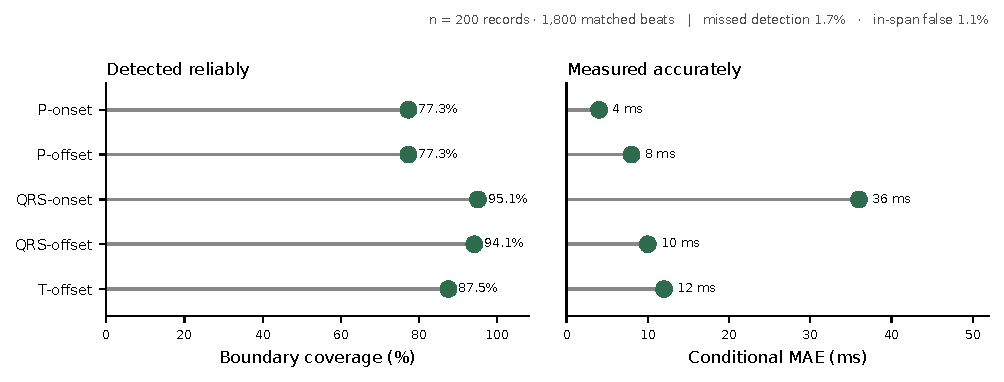
\includegraphics[width=0.9\linewidth]{figs_full/fig_s1_ludb.pdf}
\caption{\textbf{Delineation accuracy sets the measurement floor (LUDB).} The
wavelet delineator was validated against cardiologist annotations in the Lobachevsky
University database (\num{200} records, \num{1800} matched beats) with no retuning.
Left, per-boundary detection coverage; right, conditional mean absolute error against
the reference annotation. QRS onset is placed systematically early (\SI{36}{\milli\second});
all other boundaries are within \SI{12}{\milli\second}. Missed-beat rate \num{1.7}\%,
in-span false-detection rate \num{1.1}\%.}
\label{fig:s1}
\end{figure}
\clearpage

\subsection*{S2\quad Cross-cohort transfer of the phase clocks (EchoNext)}

\begin{figure}[htbp]
\centering
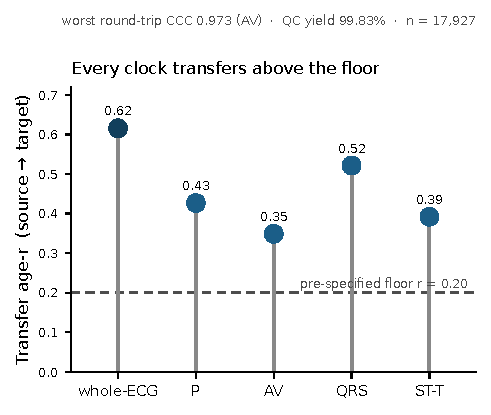
\includegraphics[width=0.85\linewidth]{figs_full/fig_s2_transfer.pdf}
\caption{\textbf{Every phase clock transfers across cohorts (EchoNext).} Correlation
between source-trained and target-cohort predicted age for the whole-ECG clock and each
of the four phase clocks ($n=\num{17927}$). All five exceed the pre-specified transfer
floor of $r=\num{0.20}$ (whole-ECG \num{0.62}, QRS \num{0.52}, P \num{0.43}, ST-T
\num{0.39}, AV \num{0.35}). Worst round-trip concordance correlation \num{0.973} (AV);
QC yield \num{99.83}\%.}
\label{fig:s2}
\end{figure}
\clearpage

\subsection*{S3\quad Exploratory per-phase effect sizes in structural disease (EchoNext)}

\begin{figure}[htbp]
\centering
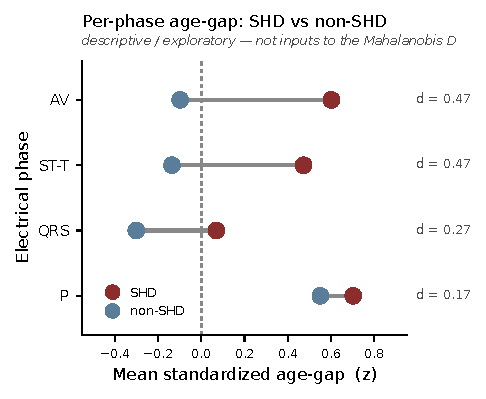
\includegraphics[width=0.8\linewidth]{figs_full/fig_s3_phase_profiles.pdf}
\caption{\textbf{Per-phase age gaps in structural disease (EchoNext, exploratory).}
Mean standardized age gap for each phase in participants with versus without
echocardiographically confirmed structural heart disease, ordered by effect size. The
AV and ST-T phases separate the groups most (Cohen's $d=\num{0.47}$ each), the atrial
phase least ($d=\num{0.17}$). This descriptive per-phase view is exploratory and is not
an input to the Mahalanobis disagreement radius \D; it motivates the phase-selective,
externally testable hypothesis discussed in the main text.}
\label{fig:s3}
\end{figure}
\clearpage

\subsection*{S4\quad Structure--function pilot (MotionVector) --- a technically limited probe}
\label{sec:motionvector}
As an exploratory probe of whether the shared-axis/orthogonal-residual construction might
extend to a structure--function pair---skeletal aging (whole-body DXA) versus seven-day
physical activity (accelerometry)---an analogous decomposition was built in the NHANES
2005--2006 participants with both modalities ($n=\num{2891}$; Methods). The prespecified
primary test, whether a calibration-orthogonal ``locomotor reserve'' predicts lower-body
physical limitation beyond age, sex, BMI and the shared axis, did not reach significance:
odds ratio \num{1.10} per contrast unit (95\% CI \numrange{0.99}{1.23}), likelihood-ratio
$p=\num{0.070}$, in the non-protective direction.

\emph{This result is not interpreted as a validated boundary finding.} The pilot has two
processing limitations that must be fixed before any conclusion is drawn (a rebuilt V2 is
future work): (i) the accelerometry features were computed from raw minute-level intensity
counts without a validated non-wear/wear-time algorithm or valid-day filtering, so they
are not comparable to accepted NHANES accelerometry processing; and (ii) the five
multiply-imputed DXA replicates were averaged into one record rather than analyzed
separately and combined by Rubin's rules, understating variance contrary to NHANES
guidance. The implemented locomotor feature set was also only a subset of the locked list
(cadence-distribution, walking-bout, fragmentation and cosinor-amplitude features were not
computed and, the outcome now being unblinded, were deliberately not added post hoc), and
the outcome is self-reported in a young cohort (ages 20--69).

With those caveats, the descriptive pattern (Fig.~\ref{fig:s4}) is the following. The two
age gaps were nearly uncorrelated ($r=\num{0.07}$; Fig.~\ref{fig:s4}a). The locomotor age
clock was a weak age predictor (out-of-fold $R^2=\num{0.17}$) whose gap correlated
\emph{positively} with daily steps ($r=+\num{0.30}$; Fig.~\ref{fig:s4}b)---more activity
mapping to an older apparent locomotor age in this age range, opposite to the protective
association of activity with function. Post-hoc, the raw ingredients were associated with
limitation in the expected directions (skeletal age gap odds ratio \num{1.14} per SD,
$p=\num{0.019}$; raw daily step count odds ratio \num{0.81} per 1000 steps,
$p<\num{1e-32}$; Fig.~\ref{fig:s4}c). These exploratory associations were computed after
the primary outcome was unblinded and are labeled as such. The pilot does not alter the
main-text A-versus-D findings and is independent of the CODE-15 confirmatory test.

\begin{figure}[htbp]
\centering
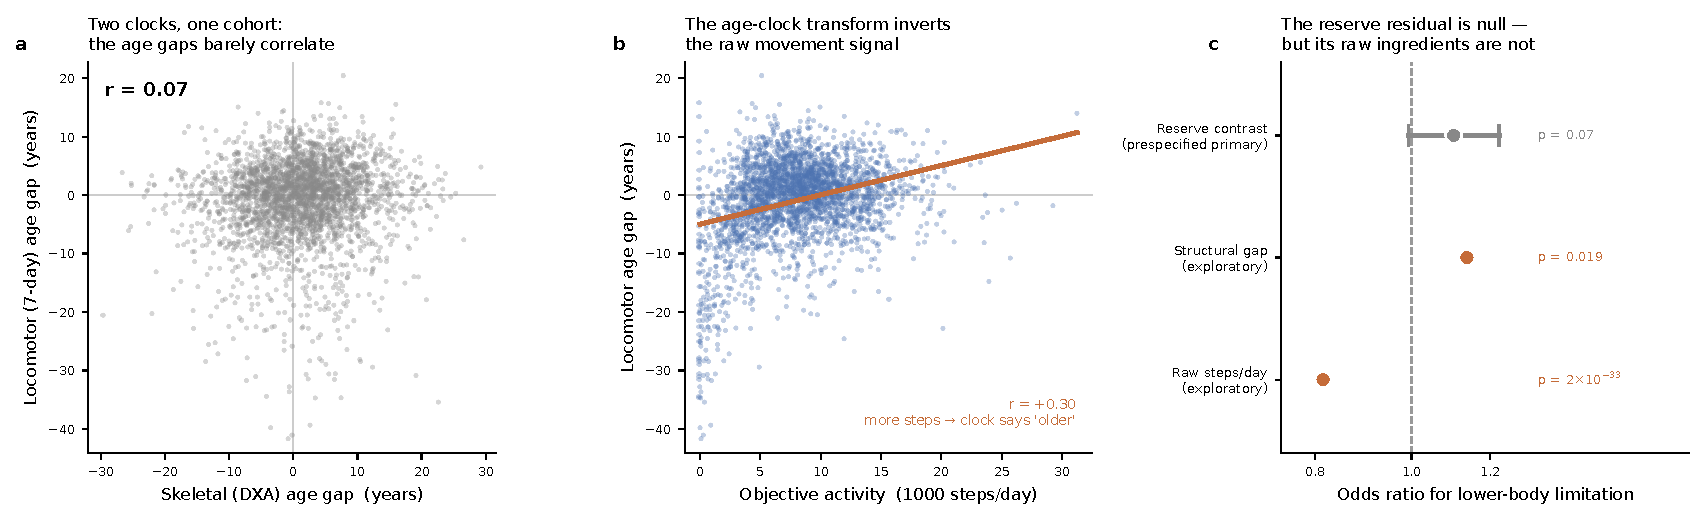
\includegraphics[width=\linewidth]{figs_full/fig_s4_motionvector.pdf}
\caption{\textbf{Structure--function pilot (NHANES 2005--2006, $n=\num{2891}$) --- a
technically limited probe, not a validated result.} Descriptive patterns only; see caveats
in \S\ref{sec:motionvector}. \textbf{(a)} The skeletal (DXA) and locomotor (seven-day
accelerometry) age gaps are nearly uncorrelated ($r=\num{0.07}$). \textbf{(b)} The
locomotor age-gap correlates positively with daily steps ($r=+\num{0.30}$)---more activity
mapping to an older apparent locomotor age, opposite to the protective role of activity.
\textbf{(c)} The prespecified ``locomotor reserve'' contrast does not reach significance
for lower-body limitation (grey; odds ratio \num{1.10} per unit, $p=\num{0.070}$,
confidence interval crossing~1); the post-hoc raw-ingredient associations (orange;
skeletal gap $p=\num{0.019}$, raw steps $p<\num{1e-32}$) were computed after unblinding and
are exploratory. Accelerometry was processed without a validated wear-time algorithm and
the DXA imputations were averaged, so these patterns are provisional.}
\label{fig:s4}
\end{figure}

\subsection*{S5\quad Brain-imaging decomposition (NeuroMotionVector)}
\label{sec:neurosupp}
As a prospective test of the decomposition at a third biological scale, the
identical shared-axis/disagreement geometry was applied to four brain-imaging channels in the Aging
Brain Cohort (AABC / HCP-Aging Release~2) with a longitudinal gait outcome and a
hash-locked, outcome-blind protocol (\S\ref{sec:neuromethods}; \S\ref{sec:neuro}). The
result was a clean null on the prespecified test: baseline brain-channel disagreement did not
predict subsequent 4-metre gait-speed decline (Fig.~\ref{fig:s8}). The four brain-age
clocks were nonetheless strong (held-out $r$ \numrange{0.50}{0.59}), and the shared axis
and disagreement radius were nearly uncorrelated, as their orthogonal-subspace construction
implies (Fig.~\ref{fig:s7}), so the null
concerns the disagreement--gait link specifically, not clock quality.

\begin{figure}[htbp]
\centering
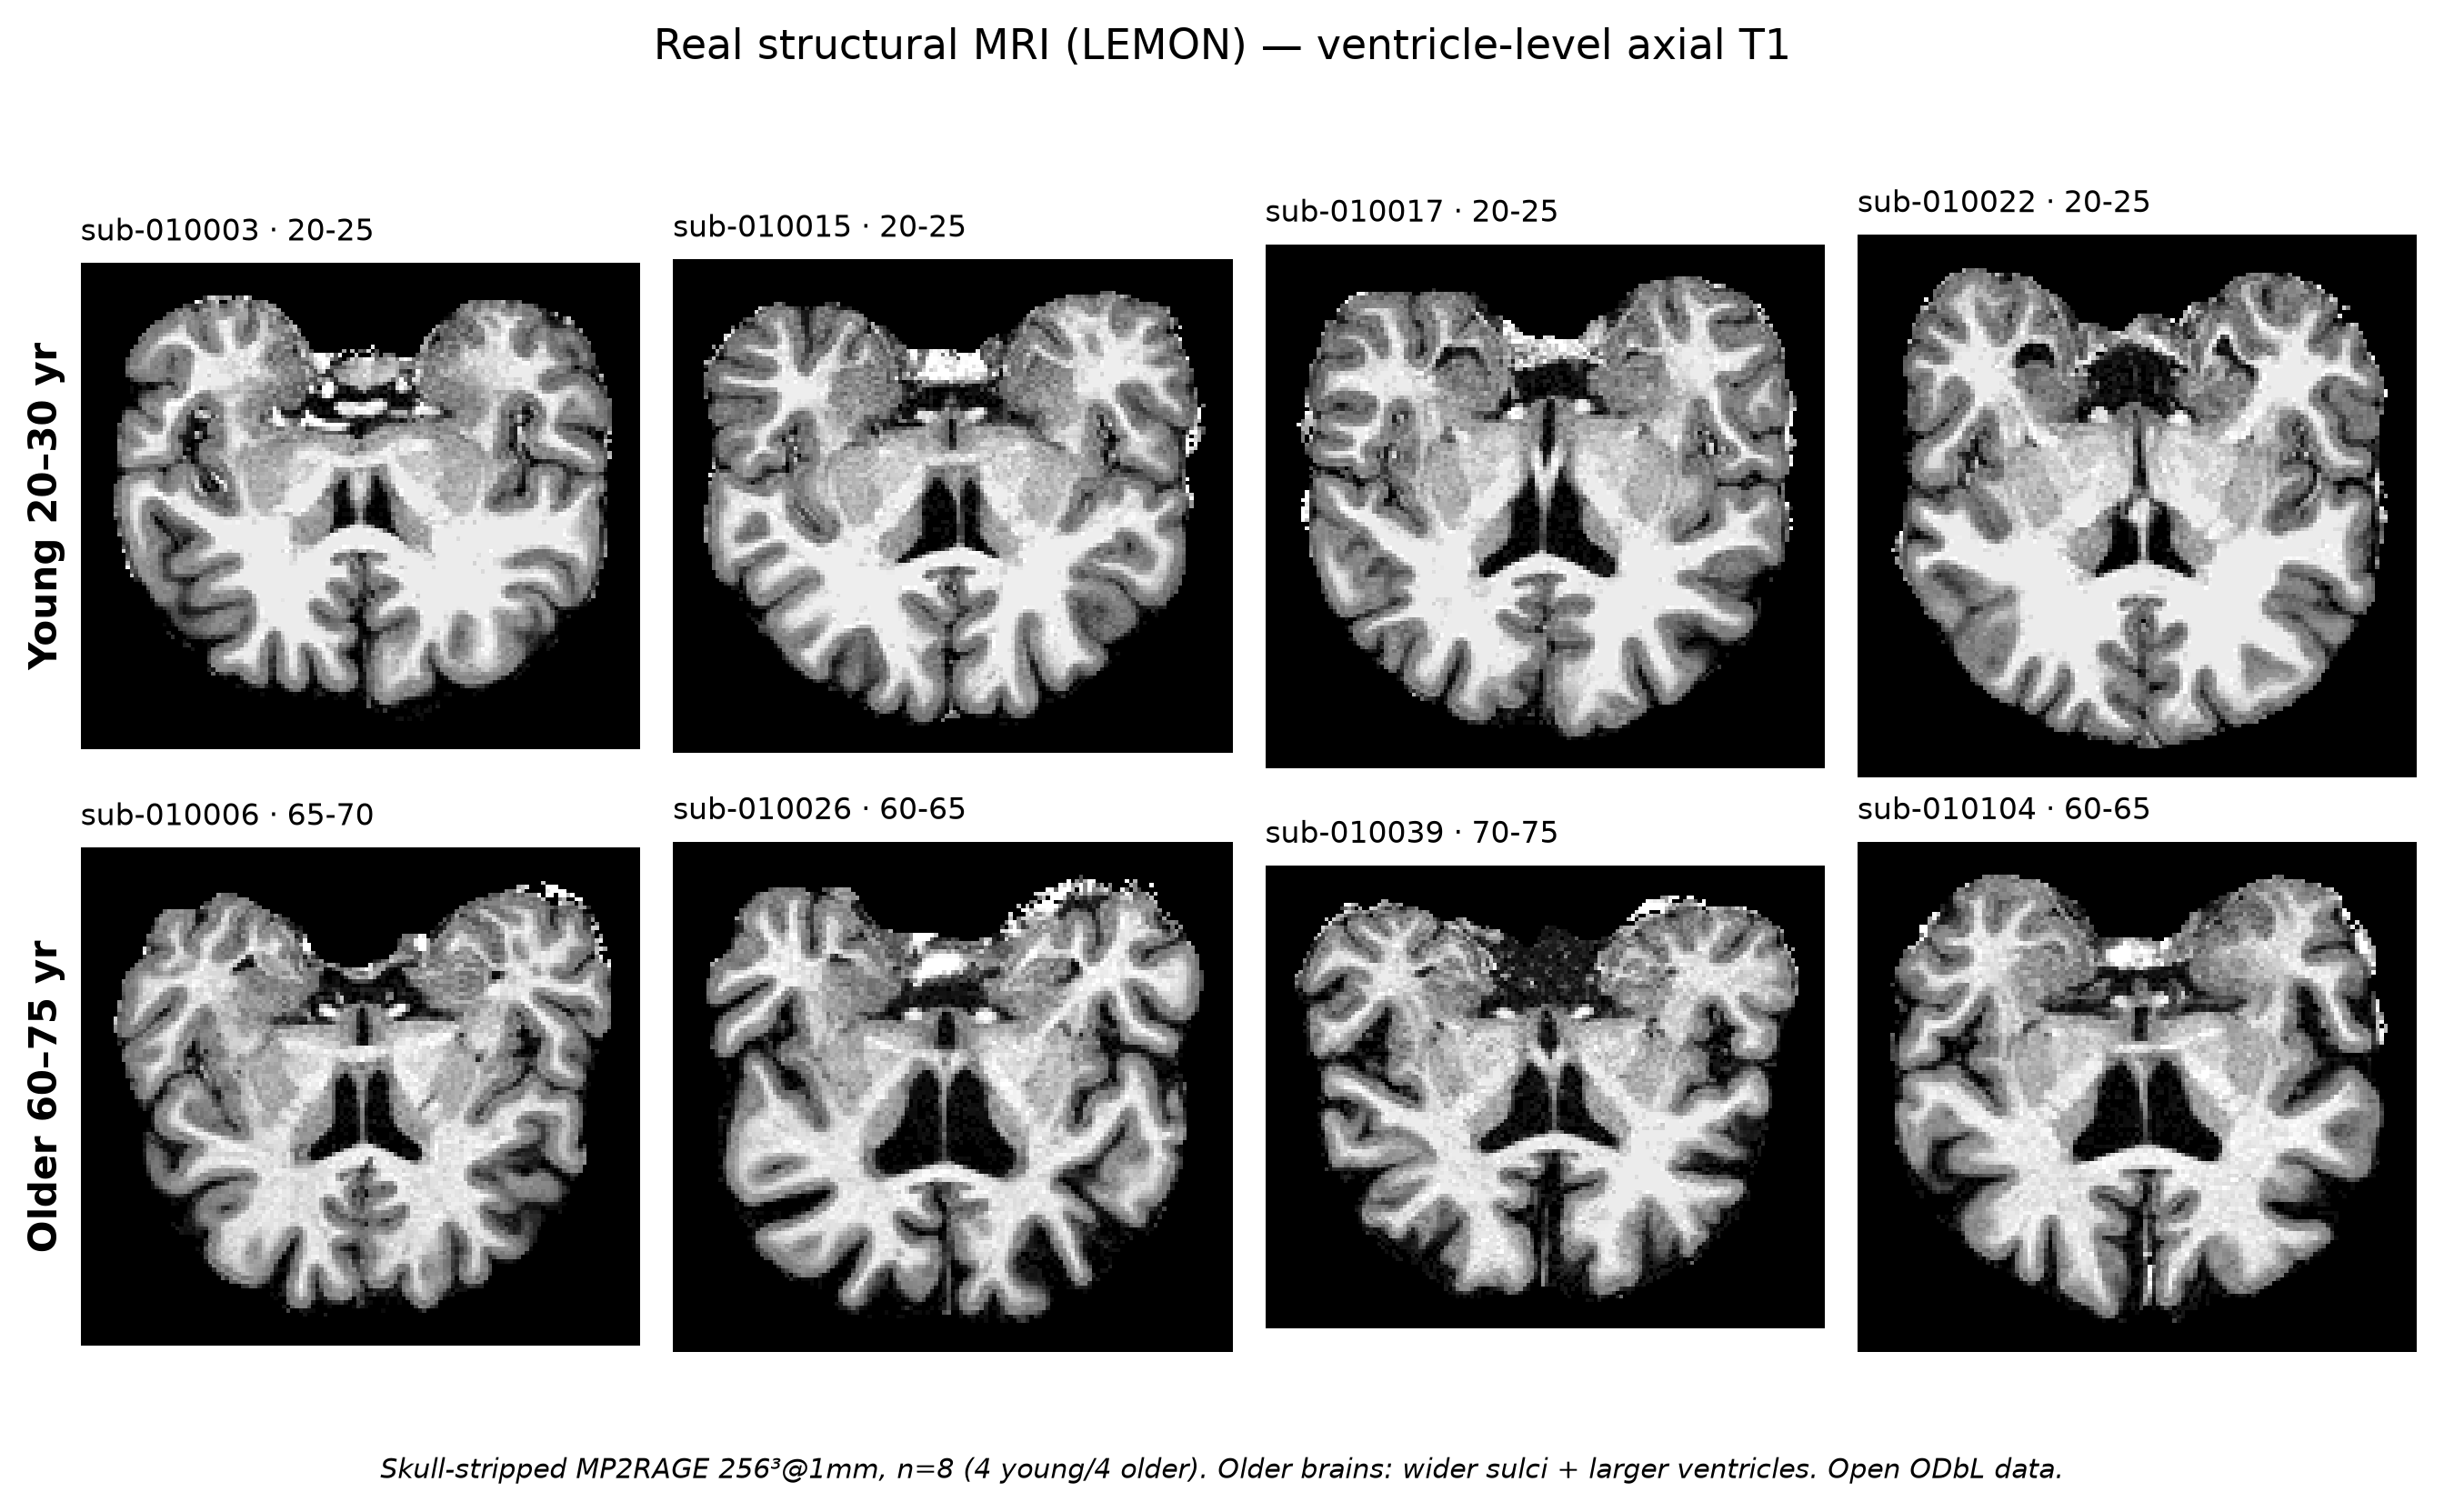
\includegraphics[width=\linewidth]{figs_full/fig_lemon_real_brains.png}
\caption{\textbf{The visible substrate of brain aging (real structural MRI, LEMON).}
Ventricle-level axial T1 slices for younger (20--30~y) versus older (60--75~y) adults from
the open-access LEMON dataset (skull-stripped MP2RAGE, $256^3$ at 1~mm). Older brains show
wider sulci and larger ventricles. These open-data images illustrate anatomy; no
controlled-access AABC scan is shown anywhere in this work.}
\label{fig:s5}
\end{figure}

\begin{figure}[htbp]
\centering
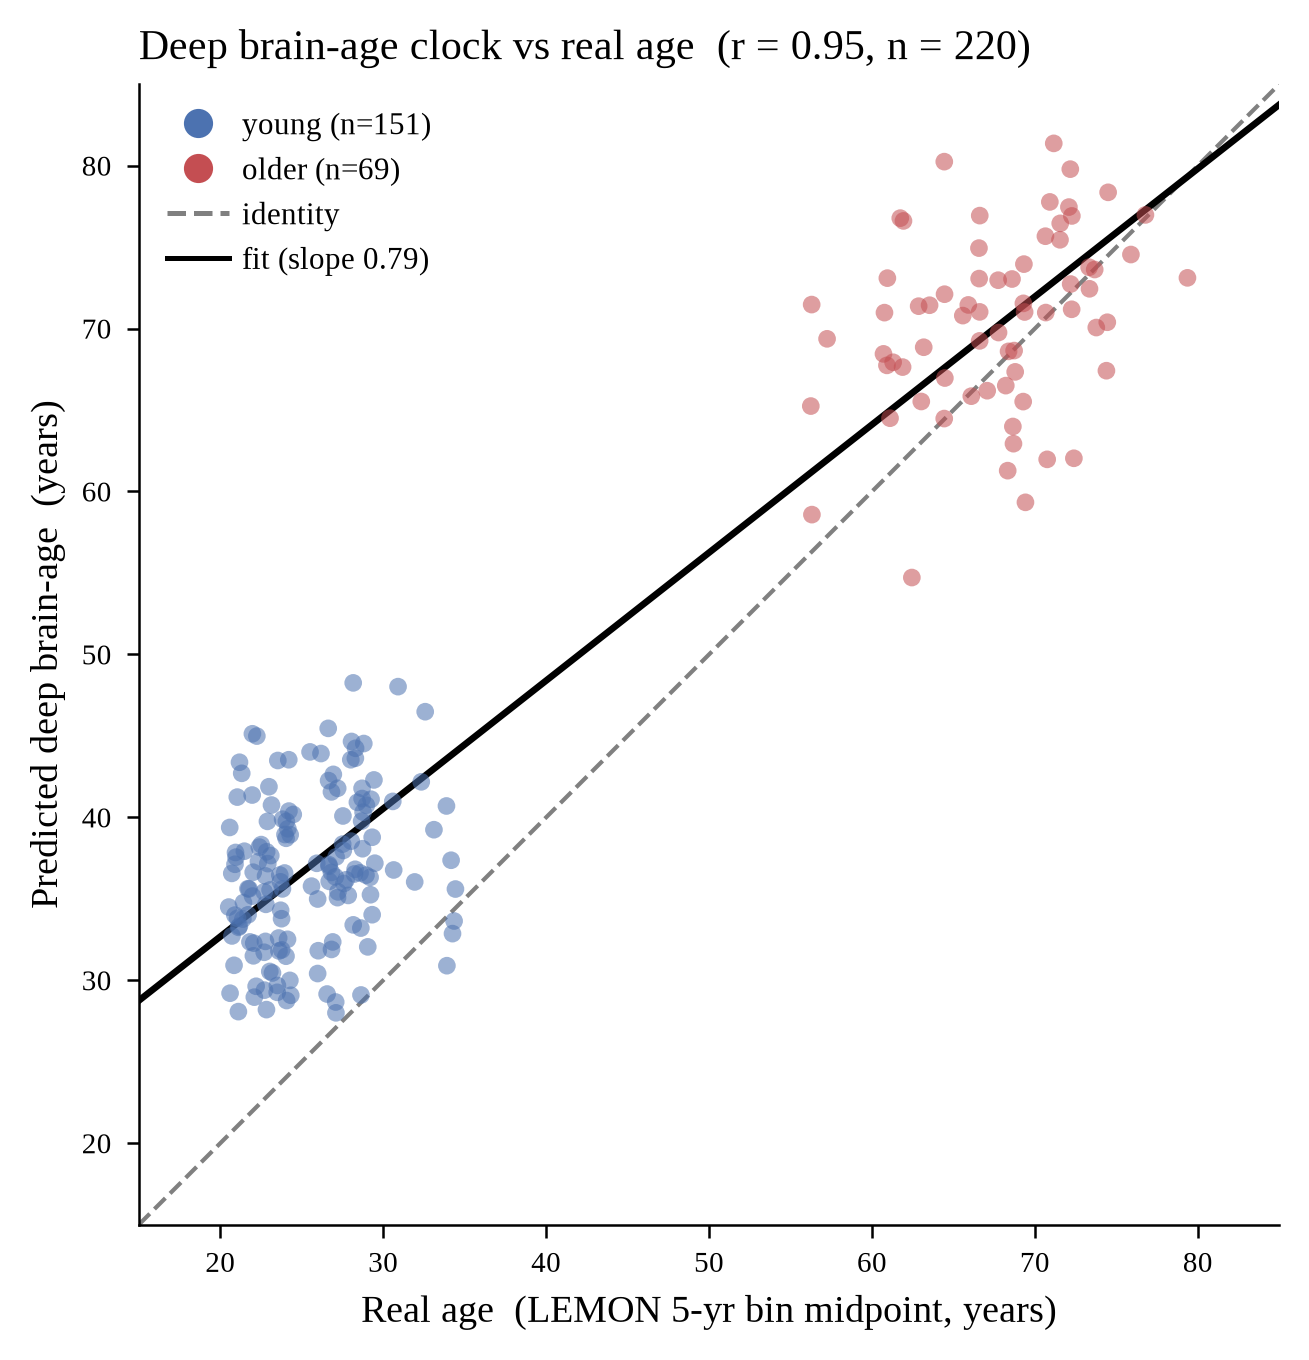
\includegraphics[width=0.7\linewidth]{figs_full/fig2_brainage_vs_realage.png}
\caption{\textbf{Deep brain-age clock validation and its domain-shift offset (LEMON).}
Predicted deep brain-age versus real age (LEMON 5-year bin midpoints) for all \num{220}
scans. The clock tracks age well in rank (Pearson $r=\num{0.95}$) but with a compressed
regression slope (\num{0.79}) and a positive offset relative to the identity line---a
textbook domain-shift bias from applying a conventional-T1w-trained model to MP2RAGE data.
Because absolute brain-age is therefore not comparable across the acquisition shift, the
image-derived disagreement analysis (\S\ref{sec:neuro}, Fig.~\ref{fig:lemon}) is specified
on the bias-invariant younger-versus-older \emph{difference} in disagreement rather than on
absolute values.}
\label{fig:lemonval}
\end{figure}

\begin{figure}[htbp]
\centering
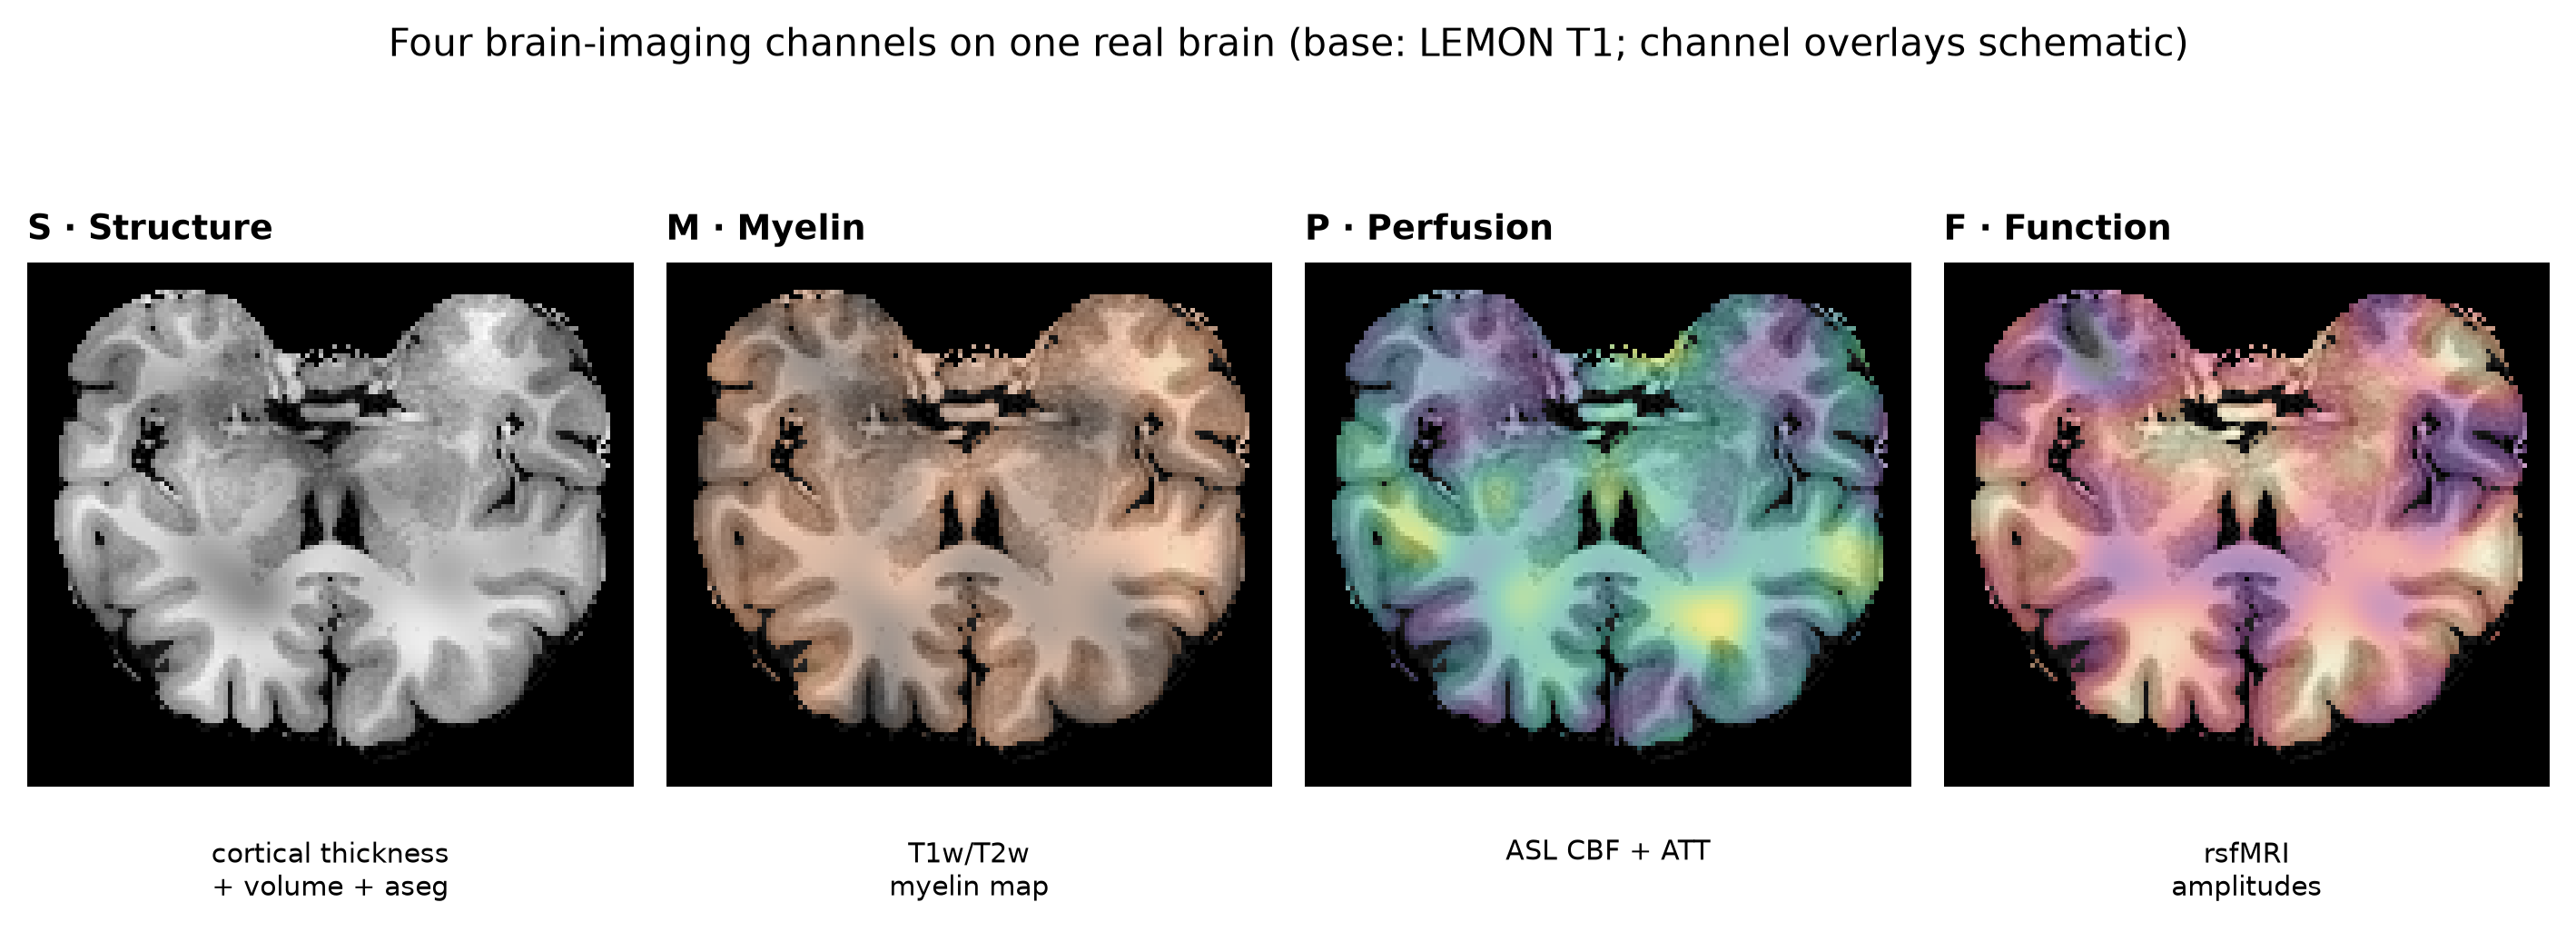
\includegraphics[width=\linewidth]{figs_full/fig_neuro_layers.png}
\caption{\textbf{Four imaging channels, one brain.} The four brain-aging views used by
NeuroMotionVector---cortical structure, T1w/T2w myelin, arterial spin-labeling perfusion,
and resting-state functional amplitude---shown as schematic overlays on a real LEMON T1
slice. Each channel is read by an independently trained age clock; their standardized age
gaps form the shared axis and disagreement radius.}
\label{fig:s6}
\end{figure}

\begin{figure}[htbp]
\centering
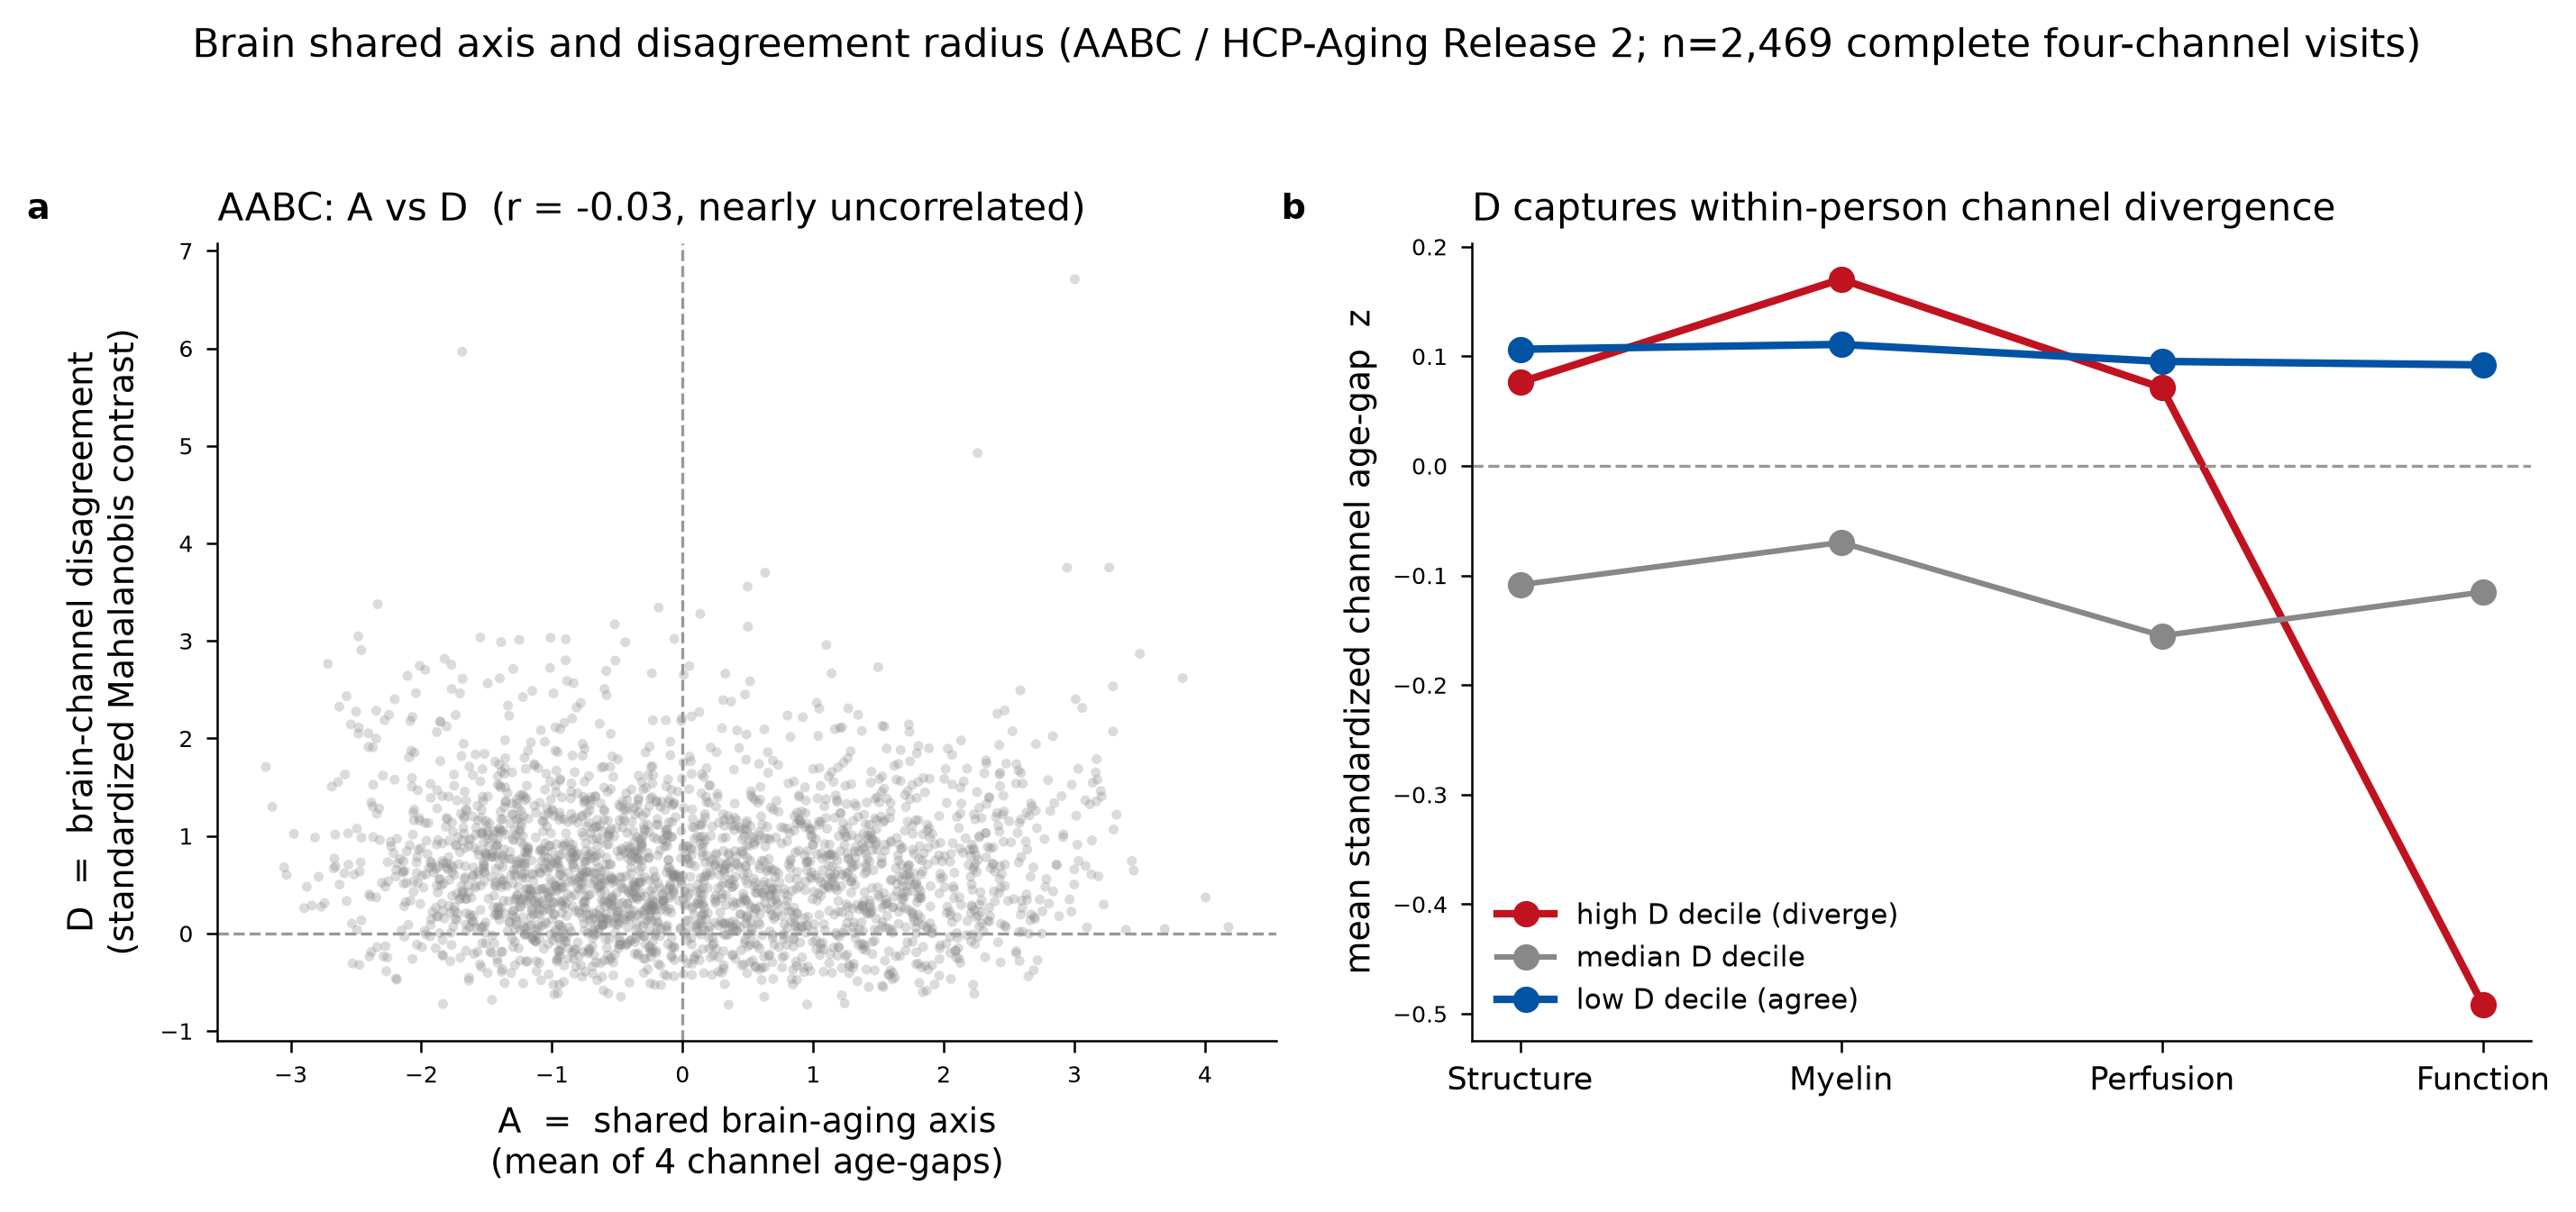
\includegraphics[width=\linewidth]{figs_full/fig_neurovector_geometry.png}
\caption{\textbf{Brain shared axis and disagreement radius (real AABC Release~2,
$n=\num{2469}$ complete four-channel visits).} \textbf{(a)} The shared brain-aging axis
$\A_{\text{brain}}$ (mean of four channel age gaps) and the disagreement radius
$\D_{\text{brain}}$ (standardized Mahalanobis contrast length) are nearly uncorrelated
($r=-\num{0.03}$), reflecting their orthogonal-subspace construction. \textbf{(b)} Participants in the highest disagreement
decile diverge sharply across channels (here a low functional age gap against older
structure/myelin), whereas low-disagreement participants track together; the disagreement
radius captures that within-person spread.}
\label{fig:s7}
\end{figure}

\begin{figure}[htbp]
\centering
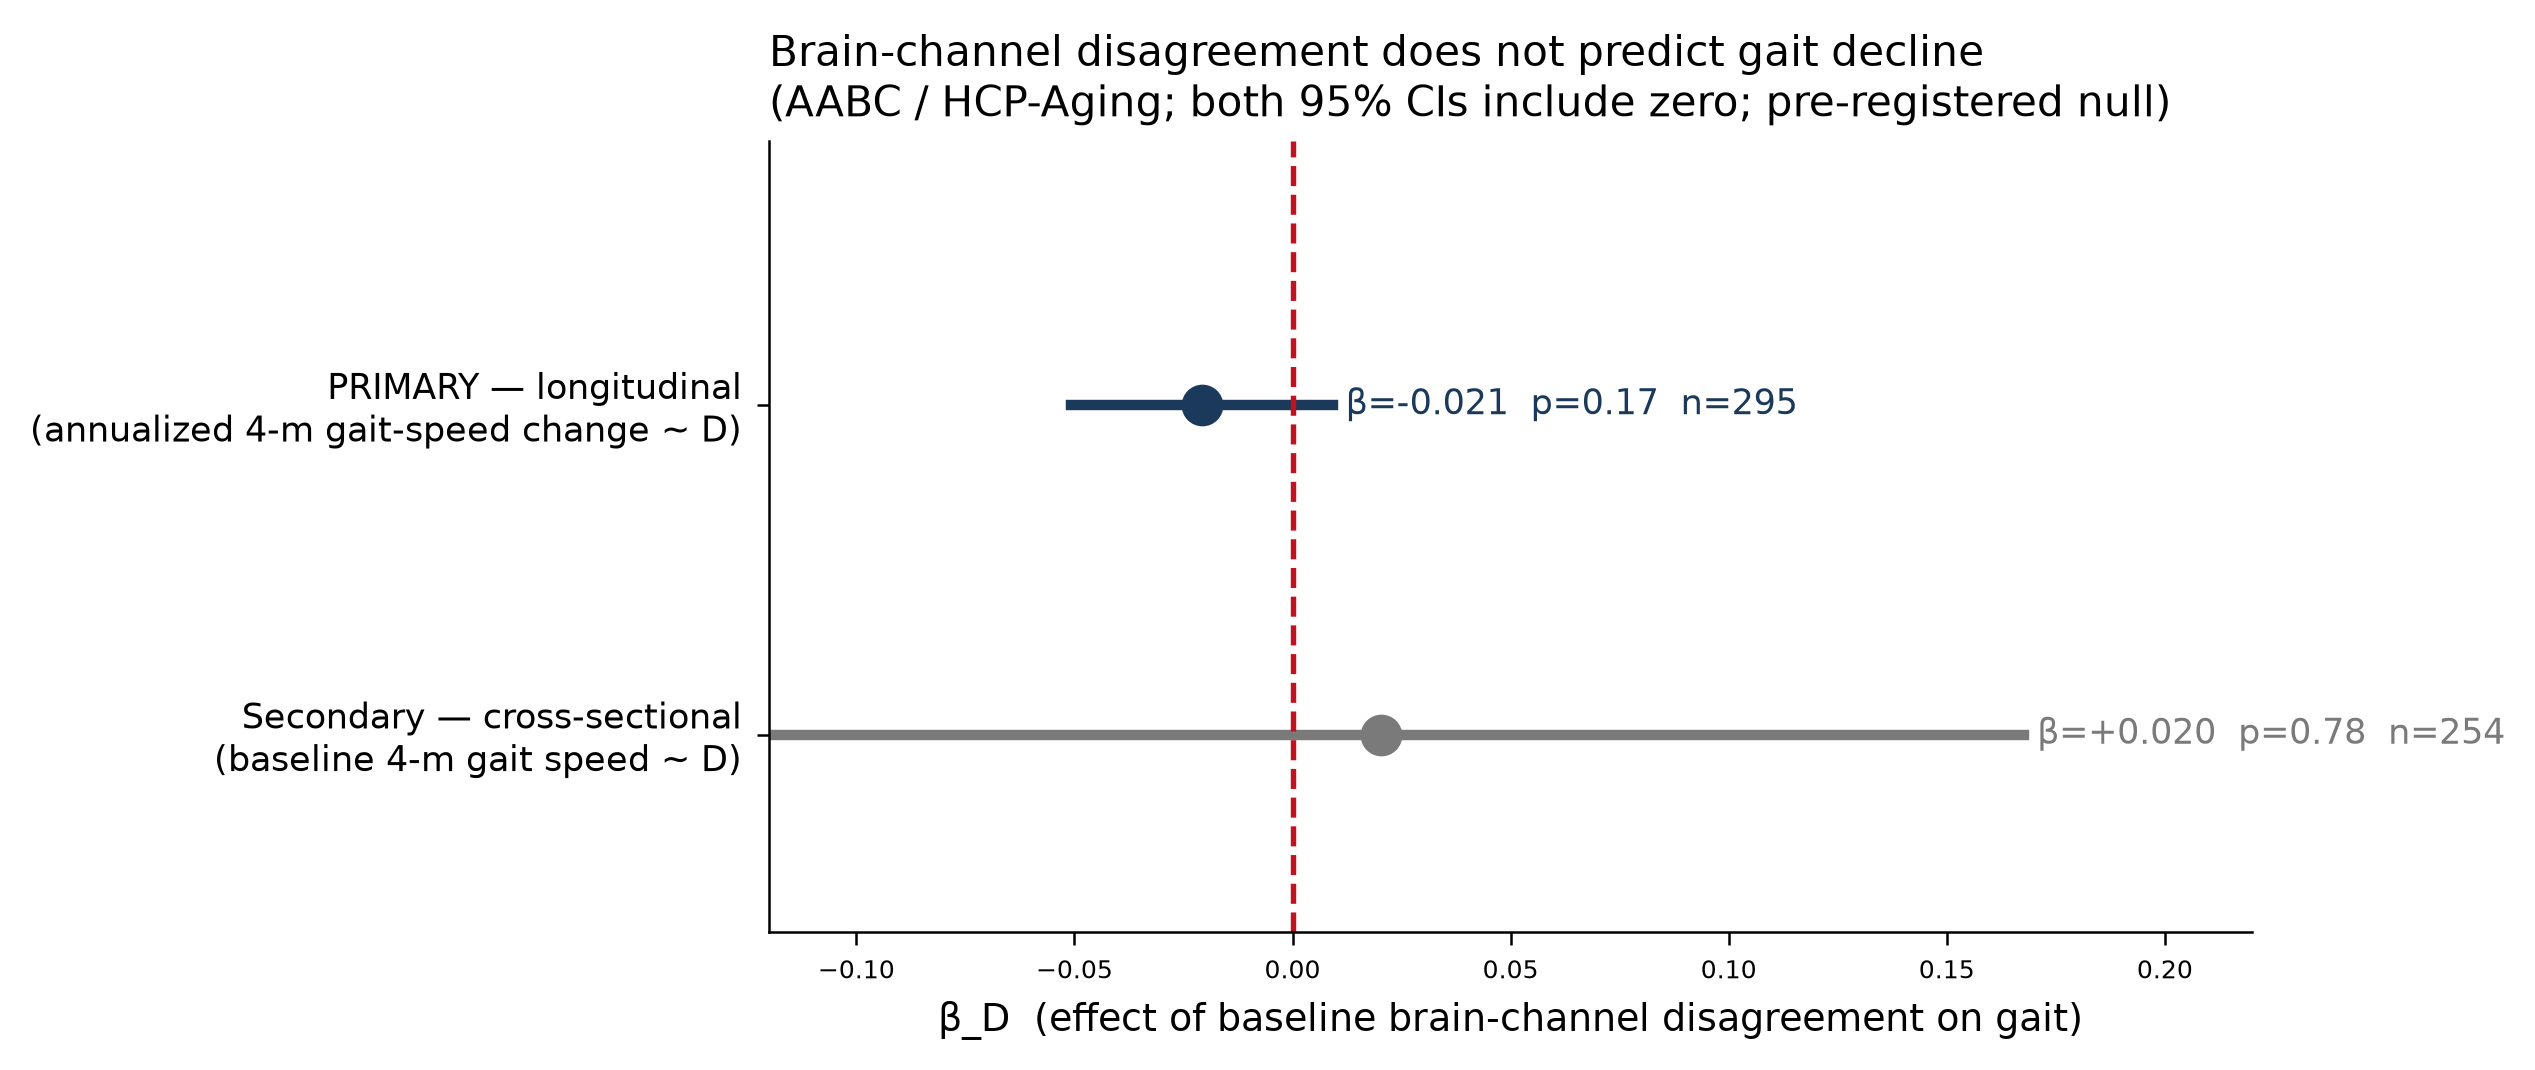
\includegraphics[width=0.9\linewidth]{figs_full/fig_neurovector_gait_result.png}
\caption{\textbf{Brain-channel disagreement does not predict gait decline (real AABC,
null on a prespecified test).} Effect of baseline brain-channel disagreement $\D_{\text{brain}}$ on
gait, per SD. The longitudinal primary (annualized 4-metre gait-speed change,
$n=\num{295}$ holdout participants) gives $\beta_D=-\num{0.021}$ (95\% CI
$[-\num{0.051},+\num{0.009}]$, $p=\num{0.17}$); the cross-sectional secondary
($n=\num{254}$) is also null ($\beta_D=+\num{0.020}$, $p=\num{0.78}$). Both confidence
intervals include zero. A single synthetic fixture with a planted disagreement--gait effect
was recovered ($p=\num{0.045}$) and a single synthetic null fixture returned null
($p=\num{0.23}$); these are a sanity check on the analysis code, not a calibration of power
or type-I error on this modest holdout.}
\label{fig:s8}
\end{figure}

\begin{figure}[htbp]
\centering
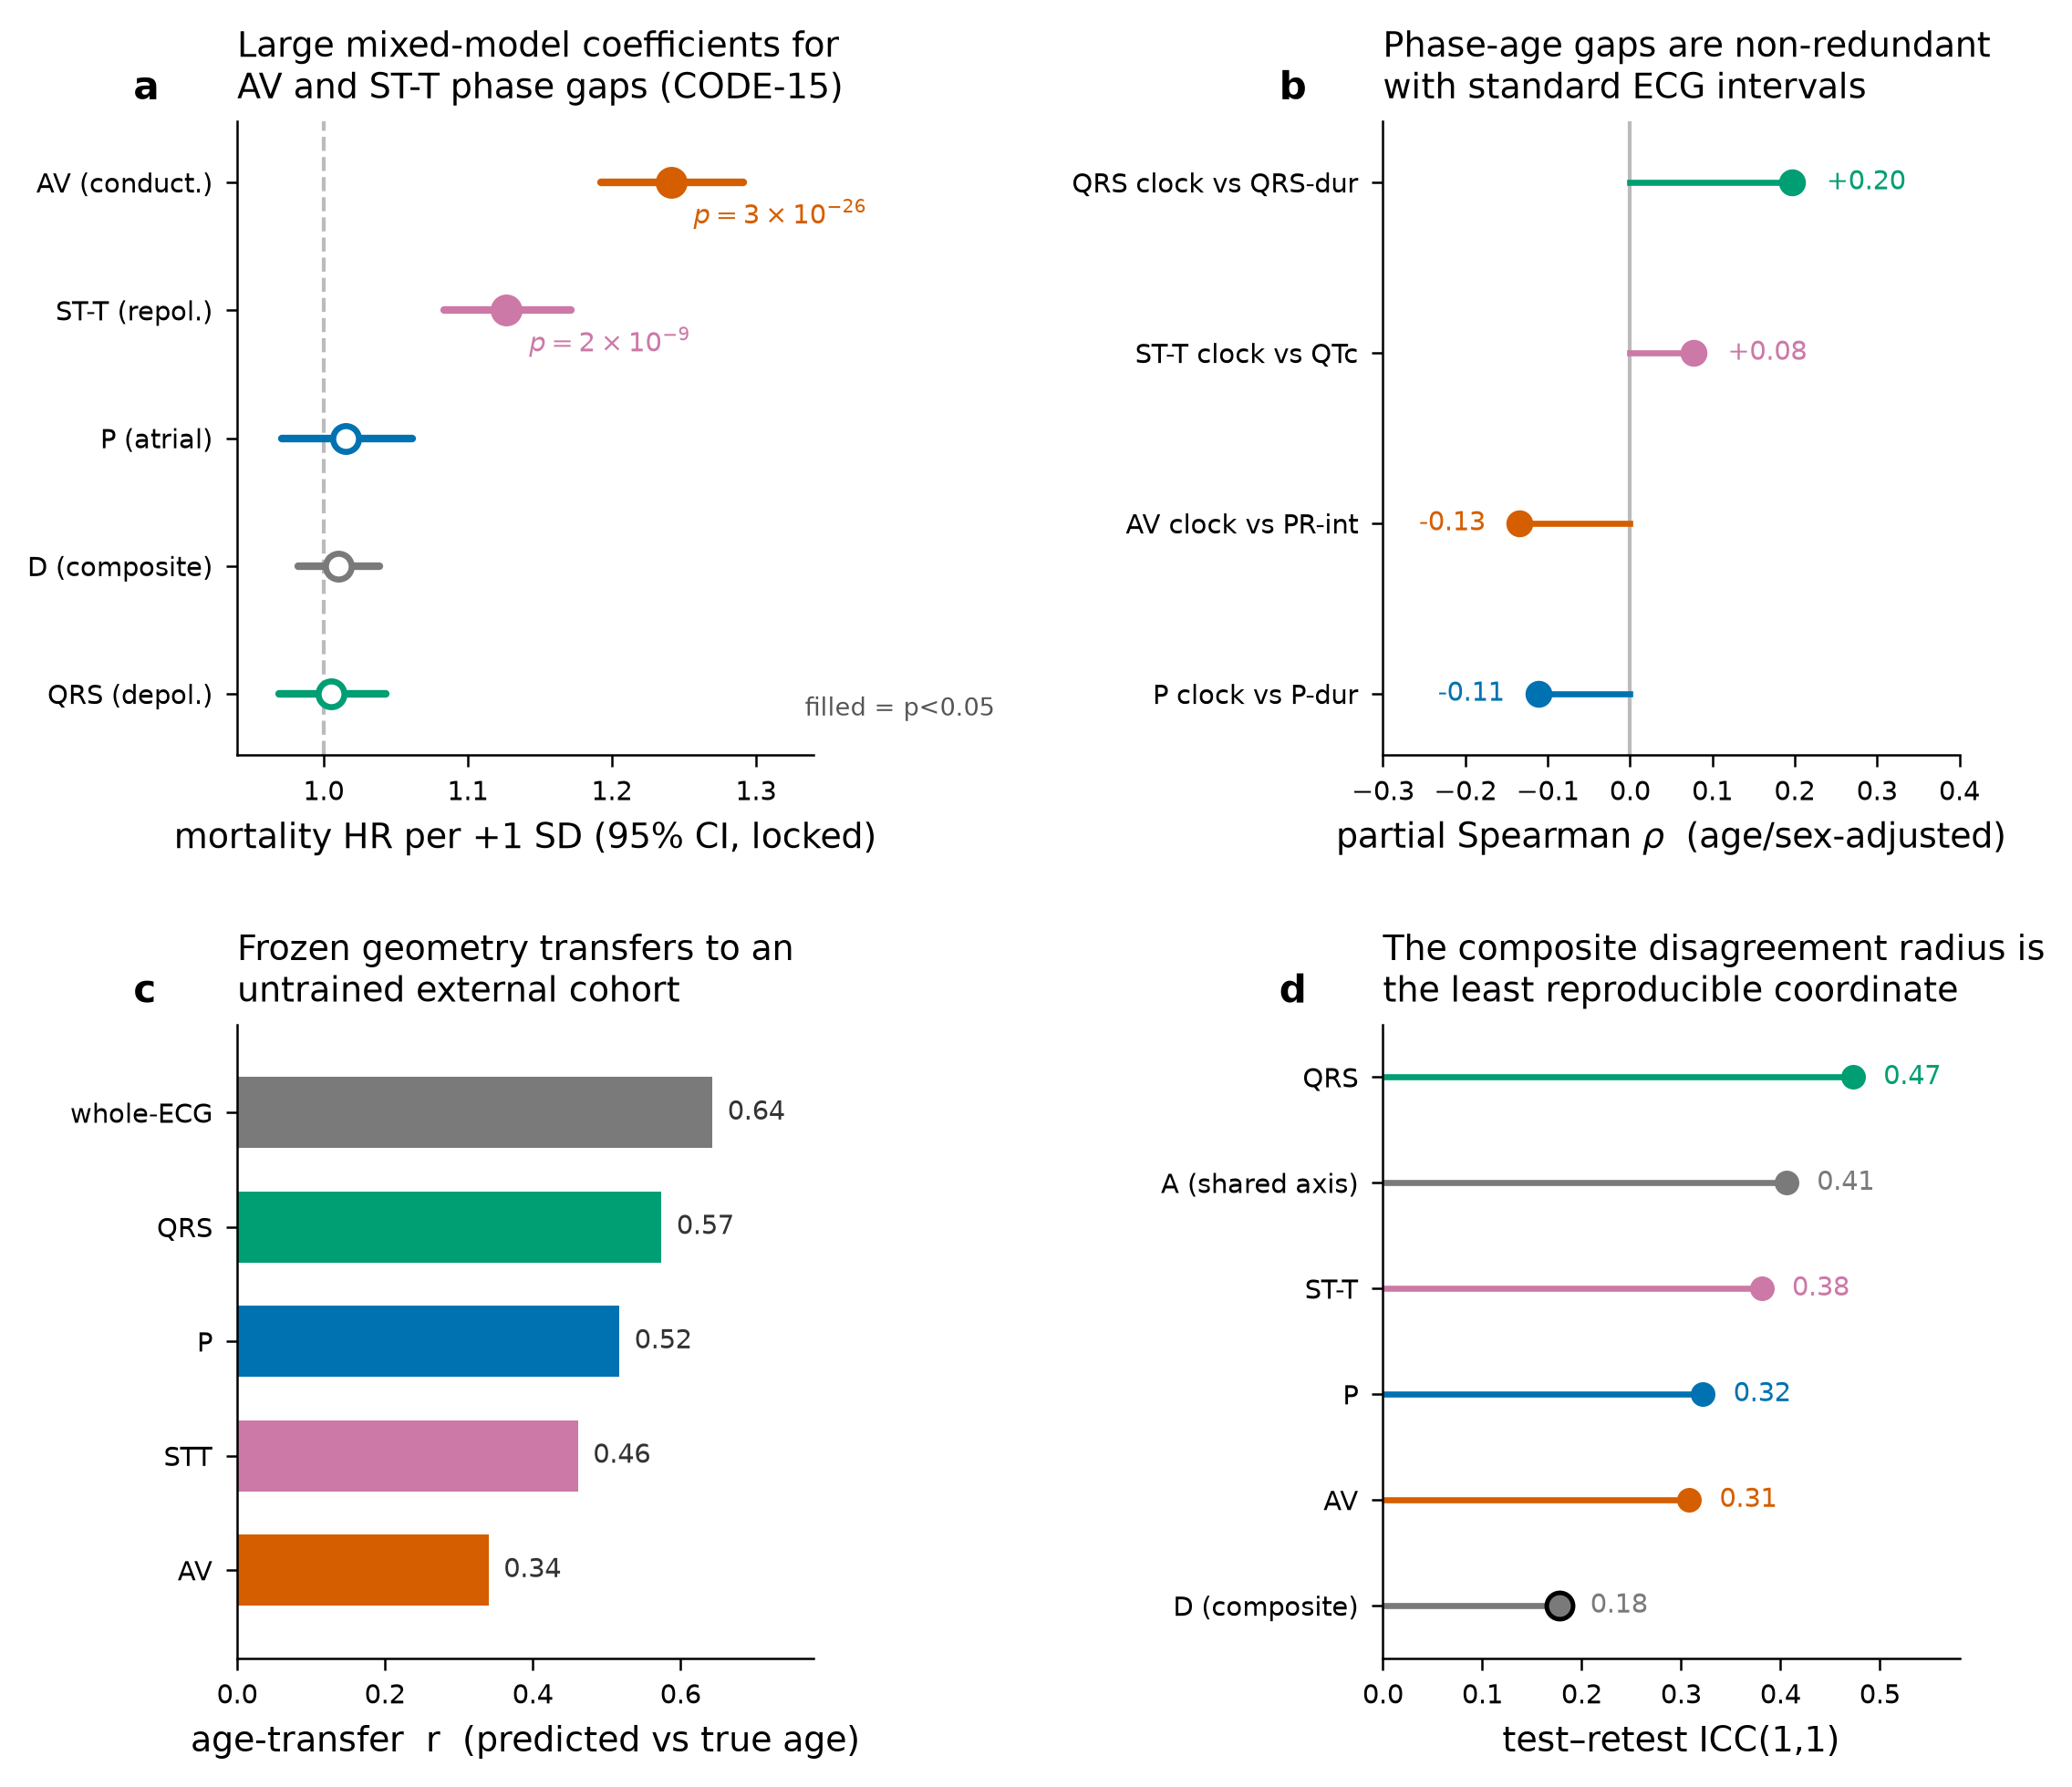
\includegraphics[width=\linewidth]{figs_full/fig_additional_analyses.png}
\caption{\textbf{Post-hoc construct-validity, transfer and reproducibility of the
electrical decomposition.} All panels use the frozen scoring pipeline with no refitting
and were computed after the confirmatory reveal.
\textbf{(a)} In a mixed shared-plus-contrast Cox model on the locked CODE-15 final split,
the atrioventricular (AV, HR $\num{1.24}$, $p=\num{3e-26}$) and ST-T repolarization (HR
$\num{1.13}$, $p=\num{2e-9}$) phase-age gaps carry large coefficients, while the atrial (P),
ventricular-depolarization (QRS) and composite disagreement radius (D) coordinates are null
(filled markers $p<\num{0.05}$; numbers re-presented from the locked reveal, not recomputed).
Because the four gaps jointly span the shared axis \A, this model does not isolate
phase-specific effects at fixed \A, and the external identifiable test (SaMi-Trop) was null;
these are therefore hypotheses rather than established effects.
\textbf{(b)} After adjusting for age and sex, each predicted phase age is only weakly
related to its matched standard interval (partial Spearman $\rho$; CODE-15 calibration,
$n=\num{74715}$), i.e.\ the phase clocks are non-redundant with standard intervals rather
than carrying incremental outcome information; the AV clock is weakly \emph{negative}
against PR interval, so its signal is not classical PR prolongation.
\textbf{(c)} The frozen geometry transfers to the untrained external Chapman--Shaoxing/Ningbo
cohort ($n=\num{44595}$ with usable age): predicted-vs-chronological age $r$ for the whole-ECG clock and each
phase clock (no mortality follow-up available, so this shows age-structure generality only).
\textbf{(d)} Within-patient test--retest reproducibility ($\mathrm{ICC}(1,1)$;
$\num{66474}$ patients, $\num{177336}$ exams): the composite disagreement radius D is the
least reproducible coordinate ($\num{0.18}$), below the shared axis A ($\num{0.41}$) and
every single-phase gap---a mechanistic complement to the confirmatory null.}
\label{fig:s9}
\end{figure}

\end{document}
